\section{Additional analysis dataset jet QA}

To explore any potential trigger dependence of these observables, the same analysis was performed using events associated solely with scaled trigger bit 18 and scaled trigger bit 34.
Trigger bit 18 and trigger bit 34 correspond to the Jet 10 trigger (trig22) plus a requirement of a minimum bias trigger (trig10 and trig12 respectively).
The results of this analysis are shown in Figures~\ref{fig:avgNjet_case2} and~\ref{fig:avgEjet_case2} for trigger bit 18 and Figures~\ref{fig:avgNjet_case3} and~\ref{fig:avgEjet_case3} for trigger bit 34.

\begin{figure}
    \centering
    \begin{subfigure}[t]{0.48\textwidth}
        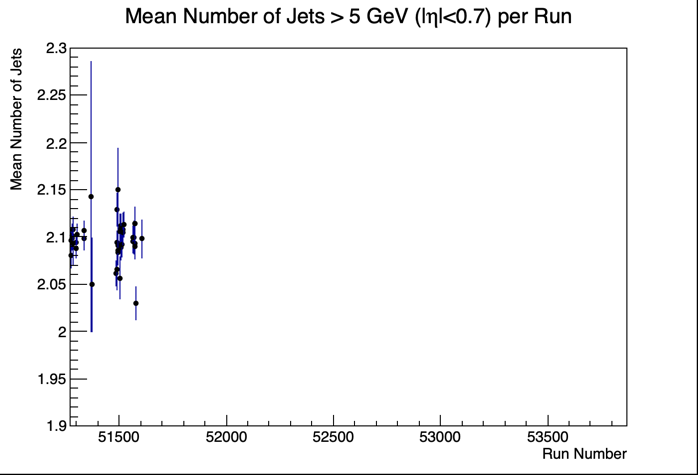
\includegraphics[width=\linewidth, trim=10 10 10 0, clip]{Figures/QA_Study/avg_njet_case8.png}
        \caption{Average number of jets per event after all selection criteria for trigger 18.}\label{fig:avgNjet_case2}
    \end{subfigure}
    \hfill
    \begin{subfigure}[t]{0.48\textwidth}
        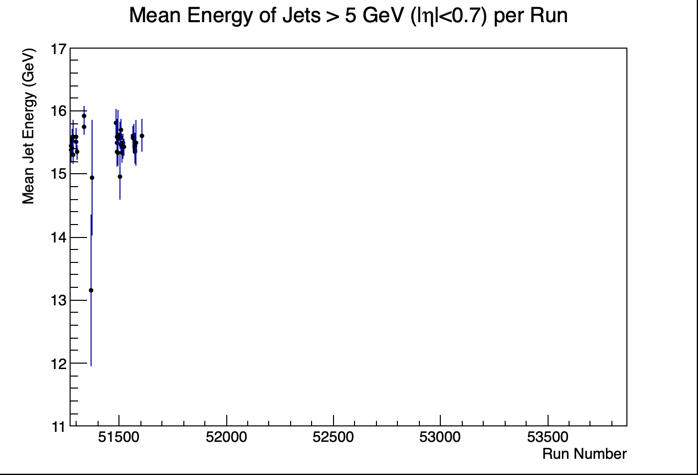
\includegraphics[width=\linewidth, trim=10 10 10 0, clip]{Figures/QA_Study/avg_ejet_case8.png}
        \caption{Average energy of jets per event after all selection criteria for trigger 18.}
        \label{fig:avgEjet_case2}
    \end{subfigure}
    \caption{Jet QA observables: (a) average number of jets per event and (b) average jet energy, after all selection cuts.}
    \label{fig:qa_jet_summary_2}
\end{figure}

The results for the trigger 18 condition are consistent with the previous findings, yielding a mean number of jets per event of approximately 2 and a mean jet energy of about 15.5~GeV.
Furthermore, the results obtained with trigger 34 are consistent with the previously observed trends, as illustrated in Figures~\ref{fig:avgNjet_case3} and~\ref{fig:avgEjet_case3}.        
The average number of jets per event remains approximately 2, and the average jet energy is around 15.5~GeV, reaffirming the stability of these observables across different trigger selections.

\begin{figure}
    \centering  
    \begin{subfigure}[t]{0.48\textwidth}
        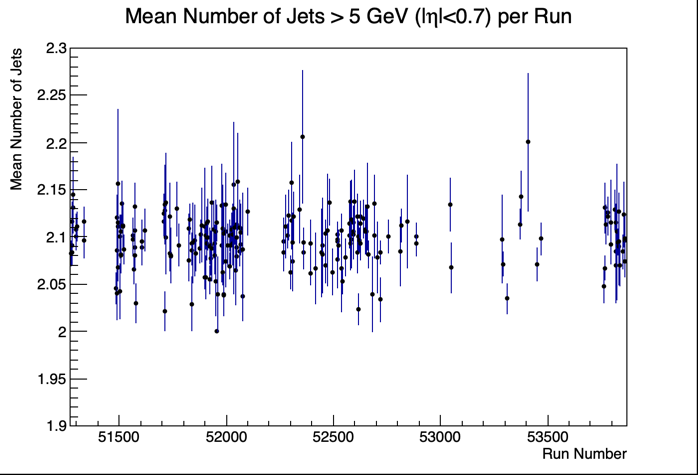
\includegraphics[width=\linewidth, trim=10 10 10 0, clip]{Figures/QA_Study/avg_njet_case9.png}
        \caption{Average number of jets per event after all selection criteria for trigger 34.}\label{fig:avgNjet_case3}
    \end{subfigure}
    \hfill
    \begin{subfigure}[t]{0.48\textwidth}
        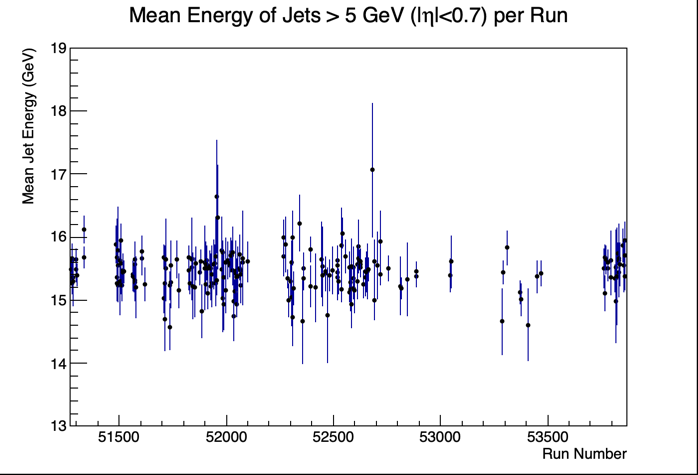
\includegraphics[width=\linewidth, trim=10 10 10 0, clip]{Figures/QA_Study/avg_ejet_case9.png}
        \caption{Average energy of jets per event after all selection criteria for trigger 34.}
        \label{fig:avgEjet_case3}
    \end{subfigure}
    \caption{Jet QA observables for trigger 34: (a) average number of jets per event and (b) average jet energy, after all selection cuts.}
    \label{fig:qa_jet_summary_3}
\end{figure}

The quality assurance (QA) of reconstructed jets in this study is assessed by analyzing the average number of jets per event and the average jet energy per event. Several selection criteria are applied to ensure clean and physically meaningful jet events.

The event selection begins with a requirement on the primary vertex \( z \)-position, constrained to \(-30~\text{cm} < z_{\text{vtx}} < +30~\text{cm}\), to reduce background from beam-induced or non-collision events. Events are required to have at least two reconstructed jets (\( N_{\text{jet}} \geq 2 \)) to ensure meaningful jet correlation studies. Furthermore, both jets used in the di-jet analysis are required to be central, with pseudorapidity \( |\eta| < 0.7 \), to minimize edge effects and maximize detector acceptance.

A di-jet azimuthal angle separation requirement of \( |\Delta\phi| \geq 3\pi/4 \) radians is imposed to select nearly back-to-back jets, consistent with hard QCD scattering processes.

Figures~\ref{fig:avgNjet_case1} and \ref{fig:avgEjet_case1} show the distributions of the average number of jets per event and the average energy of jets per event, respectively. These distributions are evaluated under the following additional criteria:
\begin{itemize}
    \item Jet transverse momentum: \( p_T > 5~\text{GeV}/c \)
    \item Trigger selection: Events must be associated with triggers in the ranges 16–23 and 32–35
    \item Leading jet transverse momentum: \( p_T^{\text{lead}} \geq 12~\text{GeV}/c \)
    \item Subleading jet transverse momentum: \( p_T^{\text{sublead}} \geq 7~\text{GeV}/c \)
\end{itemize}

\begin{figure}[h!]
    \centering
    \begin{subfigure}[t]{0.48\textwidth}
        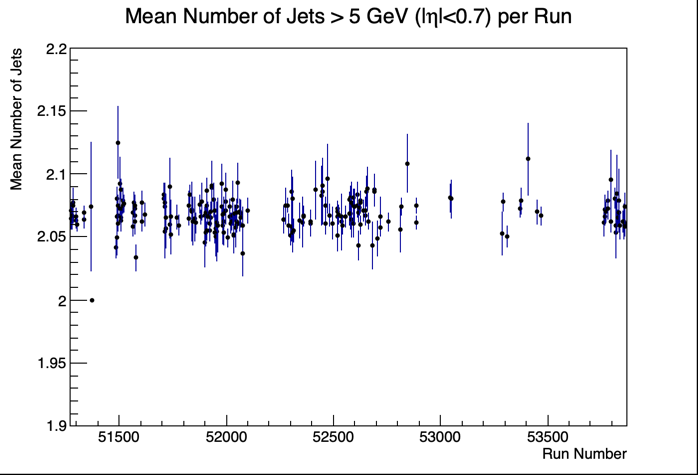
\includegraphics[width=\linewidth, trim=10 10 10 0, clip]{Figures/QA_Study/avg_njet_case1.png}
        \caption{Average number of jets per event after all selection criteria.}
        \label{fig:avgNjet_case1}
    \end{subfigure}
    \hfill
    \begin{subfigure}[t]{0.48\textwidth}
        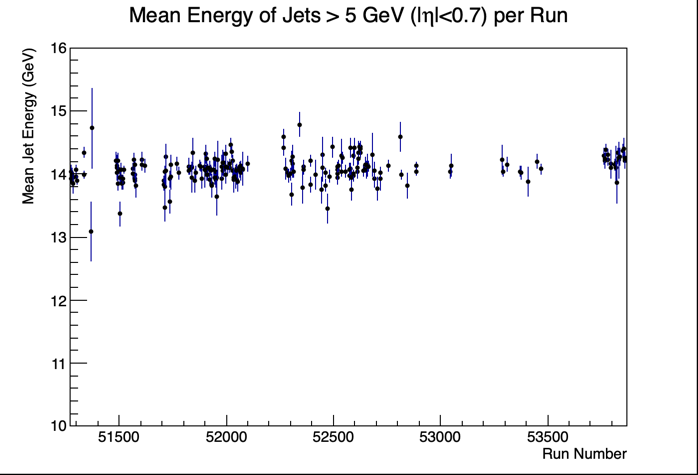
\includegraphics[width=\linewidth, trim=10 10 10 0, clip]{Figures/QA_Study/avg_ejet_case1.png}
        \caption{Average energy of jets per event after all selection criteria.}
        \label{fig:avgEjet_case1}
    \end{subfigure}
    \caption{Jet QA observables: (a) average number of jets per event and (b) average jet energy, after all selection cuts.}
    \label{fig:qa_jet_summary}
\end{figure}

The results indicate that, on average, two jets are reconstructed per event, and the average jet energy is approximately 14~GeV.

To explore the trigger dependence of these observables, the same analysis was performed using events associated solely with trigger ID 18. Figures~\ref{fig:avgNjet_case2} and~\ref{fig:avgEjet_case2} show the corresponding results under these conditions.
\begin{figure}[h!]
    \centering
    \begin{subfigure}[t]{0.48\textwidth}
        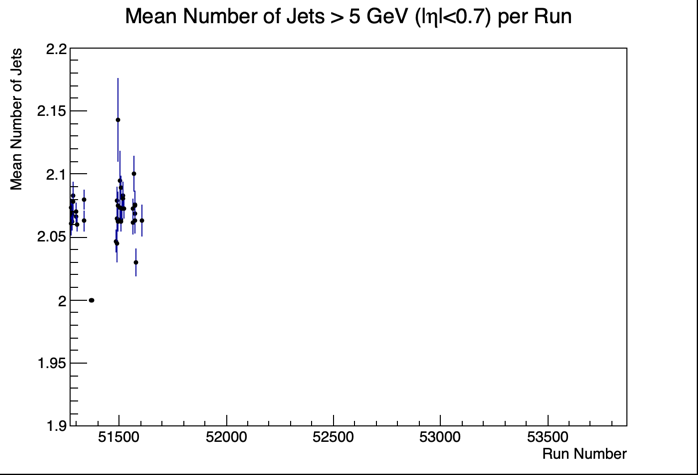
\includegraphics[width=\linewidth, trim=10 10 10 0, clip]{Figures/QA_Study/avg_njet_case2.png}
        \caption{Average number of jets per event after all selection criteria for trigger 18.}
        \label{fig:avgNjet_case2}
    \end{subfigure}
    \hfill
    \begin{subfigure}[t]{0.48\textwidth}
        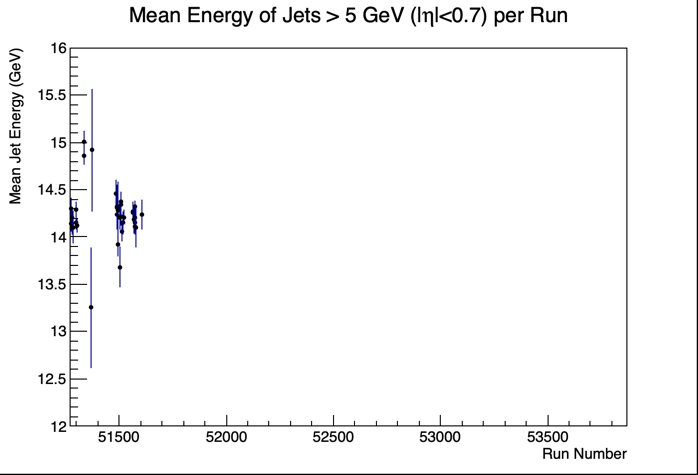
\includegraphics[width=\linewidth, trim=10 10 10 0, clip]{Figures/QA_Study/avg_ejet_case2.png}
        \caption{Average energy of jets per event after all selection criteria for trigger 18.}
        \label{fig:avgEjet_case2}
    \end{subfigure}
    \caption{Jet QA observables: (a) average number of jets per event and (b) average jet energy, after all selection cuts.}
    \label{fig:qa_jet_summary_2}
\end{figure}
The results for the trigger 18 condition are consistent with the previous findings, yielding a mean number of jets per event of approximately 2 and a mean jet energy of about 14~GeV.
Furthermore, the results obtained with trigger 34 are consistent with the previously observed trends, as illustrated in Figures~\ref{fig:avgNjet_case3} and~\ref{fig:avgEjet_case3}. The average number of jets per event remains approximately 2, and the average jet energy is around 14~GeV, reaffirming the stability of these observables across different trigger selections.

\begin{figure}[h!]
    \centering
    \begin{subfigure}[t]{0.48\textwidth}
        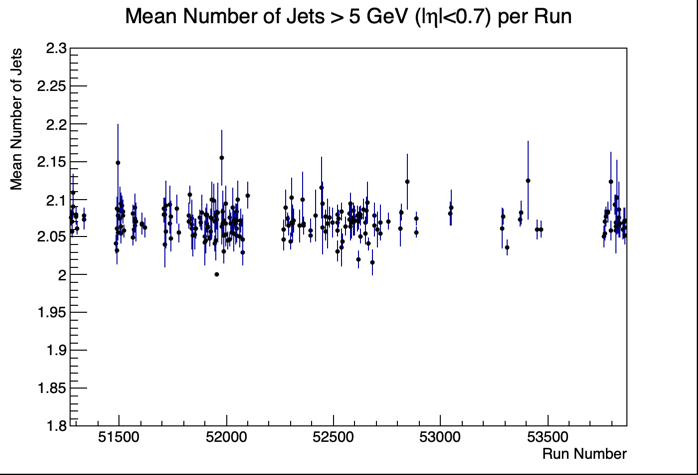
\includegraphics[width=\linewidth, trim=10 10 10 0, clip]{Figures/QA_Study/avg_njet_case3.png}
        \caption{Average number of jets per event after all selection criteria for trigger 34.}
        \label{fig:avgNjet_case3}
    \end{subfigure}
    \hfill
    \begin{subfigure}[t]{0.48\textwidth}
        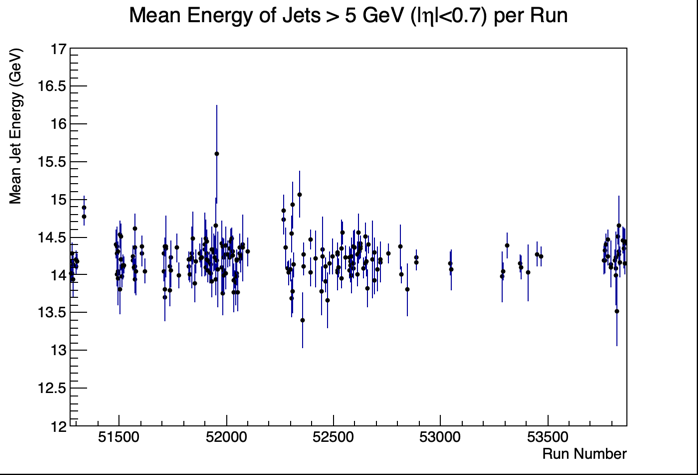
\includegraphics[width=\linewidth, trim=10 10 10 0, clip]{Figures/QA_Study/avg_ejet_case3.png}
        \caption{Average energy of jets per event after all selection criteria for trigger 34.}
        \label{fig:avgEjet_case3}
    \end{subfigure}
    \caption{Jet QA observables for trigger 34: (a) average number of jets per event and (b) average jet energy, after all selection cuts.}
    \label{fig:qa_jet_summary_3}
\end{figure}
In order to further investigate jet characteristics under less restrictive angular separation conditions, an additional set of QA studies was conducted using a modified azimuthal angle separation criterion of \( \Delta\phi = \frac{3\pi}{4} \) radians. This allows the inclusion of jet pairs that are not strictly back-to-back, thereby extending the phase space considered in the analysis. The transverse momentum selection for jets in this case remains stringent: the leading jet is required to have \( p_T^{\text{lead}} > 12~\mathrm{GeV}/c \), while the subleading jet must satisfy \( p_T^{\text{sublead}} > 0.3 \times p_T^{\text{lead}} \). These additional conditions aim to ensure the presence of significant subleading jet activity while permitting flexibility in jet topology.

Figures~\ref{fig:avgNjet_case4} and~\ref{fig:avgEjet_case4} present the distributions of the average number of jets per event and average jet energy, respectively, for events triggered within the ranges 16–23 and 32–35. The same observables are shown for events selected with trigger 18 in Figures~\ref{fig:avgNjet_case5} and~\ref{fig:avgEjet_case5}, and for trigger 34 in Figures~\ref{fig:avgNjet_case6} and~\ref{fig:avgEjet_case6}. In all cases, the results remain consistent with previous observations: the mean number of jets per event is approximately 2, while the average jet energy per event is slightly lower, around 13~GeV. These findings demonstrate the robustness of the reconstructed jet observables under varying topological and trigger constraints.

\begin{figure}[H]
    \centering
    \begin{subfigure}[t]{0.48\textwidth}
        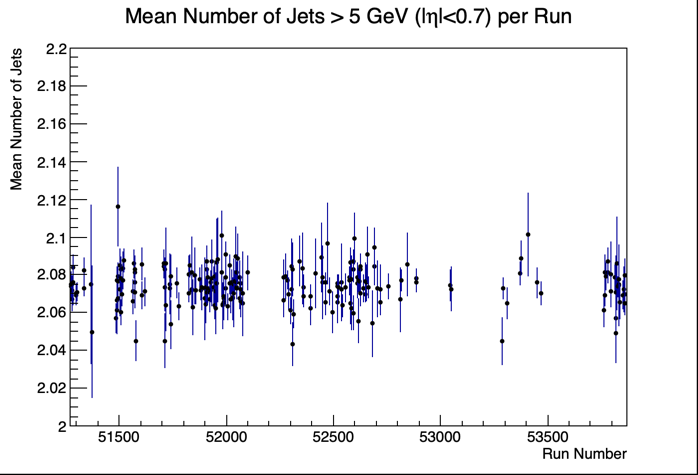
\includegraphics[width=\linewidth, trim=10 10 10 0, clip]{Figures/QA_Study/avg_njet_case4.png}
        \caption{Average number of jets per event for triggers 16–23 and 32–35, with \(\Delta\phi = 3\pi/4\) and \(p_T^{\text{sublead}} > 0.3 \times p_T^{\text{lead}}\).}
        \label{fig:avgNjet_case4}
    \end{subfigure}
    \hfill
    \begin{subfigure}[t]{0.48\textwidth}
        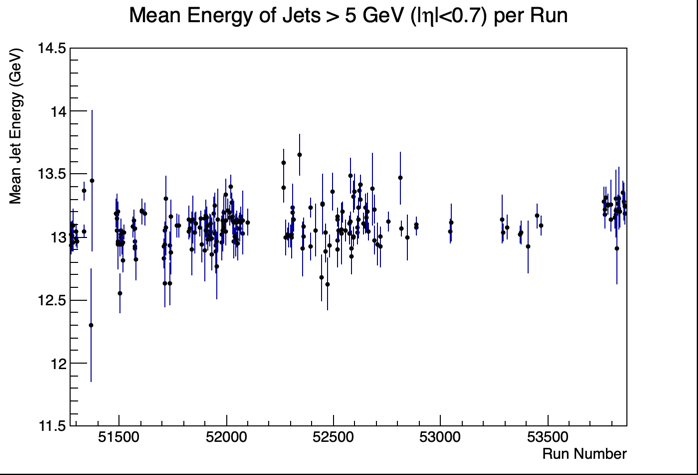
\includegraphics[width=\linewidth, trim=10 10 10 0, clip]{Figures/QA_Study/avg_ejet_case4.png}
        \caption{Average jet energy per event for triggers 16–23 and 32–35 under same conditions.}
        \label{fig:avgEjet_case4}
    \end{subfigure}
    \caption{Jet QA observables under relaxed angular separation condition (\(\Delta\phi = 3\pi/4\)) and scaled subleading jet threshold, for triggers 16–23 and 32–35.}
    \label{fig:qa_jet_summary_4}
\end{figure}
\begin{figure}[H]
    \centering
    \begin{subfigure}[t]{0.48\textwidth}
        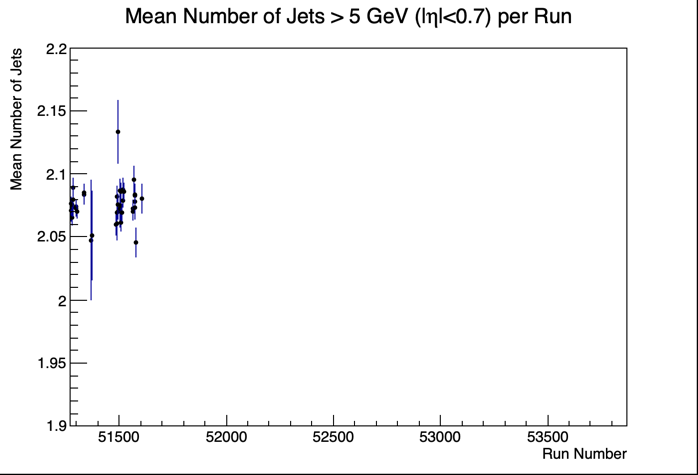
\includegraphics[width=\linewidth, trim=10 10 10 0, clip]{Figures/QA_Study/avg_njet_case5.png}
        \caption{Average number of jets per event for trigger 18, with \(\Delta\phi = 3\pi/4\) and \(p_T^{\text{sublead}} > 0.3 \times p_T^{\text{lead}}\).}
        \label{fig:avgNjet_case5}
    \end{subfigure}
    \hfill
    \begin{subfigure}[t]{0.48\textwidth}
        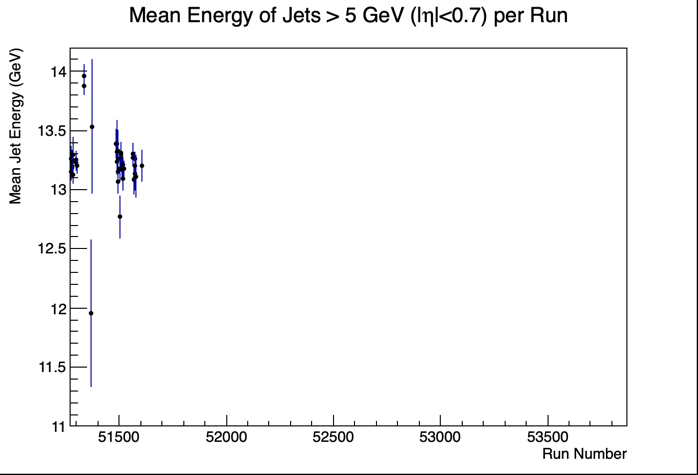
\includegraphics[width=\linewidth, trim=10 10 10 0, clip]{Figures/QA_Study/avg_ejet_case5.png}
        \caption{Average jet energy per event for trigger 18 under same conditions.}
        \label{fig:avgEjet_case5}
    \end{subfigure}
    \caption{Jet QA observables under relaxed \(\Delta\phi\) and scaled subleading jet \(p_T\) threshold, for trigger 18.}
    \label{fig:qa_jet_summary_5}
\end{figure}
\begin{figure}[H]
    \centering
    \begin{subfigure}[t]{0.48\textwidth}
        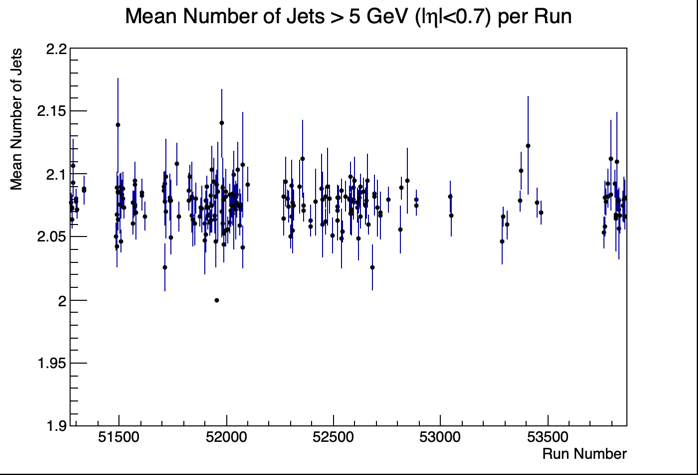
\includegraphics[width=\linewidth, trim=10 10 10 0, clip]{Figures/QA_Study/avg_njet_case6.png}
        \caption{Average number of jets per event for trigger 34, with \(\Delta\phi = 3\pi/4\) and \(p_T^{\text{sublead}} > 0.3 \times p_T^{\text{lead}}\).}
        \label{fig:avgNjet_case6}
    \end{subfigure}
    \hfill
    \begin{subfigure}[t]{0.48\textwidth}
        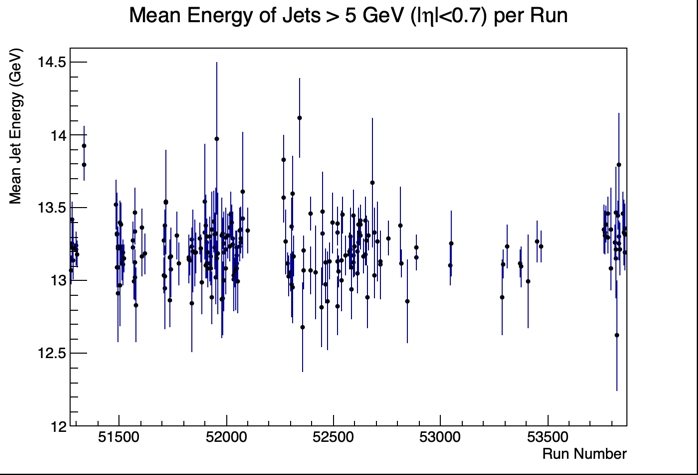
\includegraphics[width=\linewidth, trim=10 10 10 0, clip]{Figures/QA_Study/avg_ejet_case6.png}
        \caption{Average jet energy per event for trigger 34 under same conditions.}
        \label{fig:avgEjet_case6}
    \end{subfigure}
    \caption{Jet QA observables under relaxed angular and subleading jet conditions, for trigger 34.}
    \label{fig:qa_jet_summary_6}
\end{figure}
To further probe the impact of higher jet energy thresholds on jet reconstruction performance, a final QA study was conducted with a more stringent selection on the leading jet transverse momentum: \( p_T^{\text{lead}} > 15~\mathrm{GeV}/c \), while maintaining the subleading jet condition \( p_T^{\text{sublead}} > 0.3 \times p_T^{\text{lead}} \) and a relaxed azimuthal angular separation of \( \Delta\phi = \frac{3\pi}{4} \). This configuration emphasizes events with harder jet activity while still allowing broader angular correlations.

Figures~\ref{fig:avgNjet_case7} and~\ref{fig:avgEjet_case7} present the average number of jets per event and the average jet energy, respectively, for events triggered with IDs in the ranges 16–23 and 32–35. The corresponding results for trigger 18 are shown in Figures~\ref{fig:avgNjet_case8} and~\ref{fig:avgEjet_case8}, and for trigger 34 in Figures~\ref{fig:avgNjet_case9} and~\ref{fig:avgEjet_case9}. The findings are consistent across all trigger categories: the mean number of jets per event remains approximately 2, and the average jet energy per event increases to around 15~GeV, as expected given the more stringent leading jet threshold.

\begin{figure}[H]
    \centering
    \begin{subfigure}[t]{0.48\textwidth}
        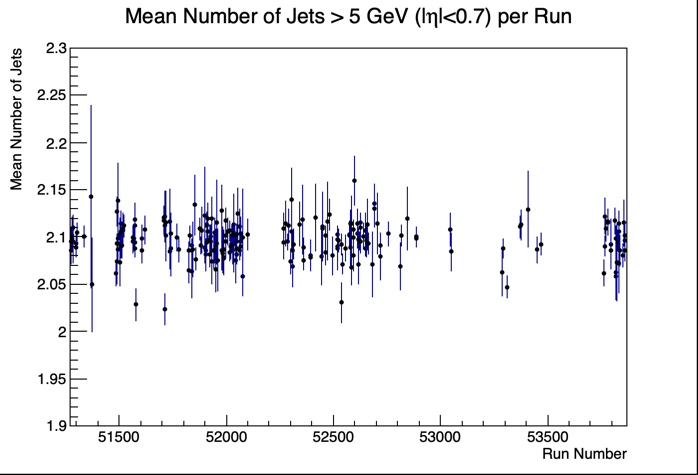
\includegraphics[width=\linewidth, trim=10 10 10 0, clip]{Figures/QA_Study/avg_njet_case7.png}
        \caption{Average number of jets per event for triggers 16–23 and 32–35, with \(p_T^{\text{lead}} > 15~\mathrm{GeV}/c\), \(p_T^{\text{sublead}} > 0.3 \times p_T^{\text{lead}}\), and \(\Delta\phi = 3\pi/4\).}
        \label{fig:avgNjet_case7}
    \end{subfigure}
    \hfill
    \begin{subfigure}[t]{0.48\textwidth}
        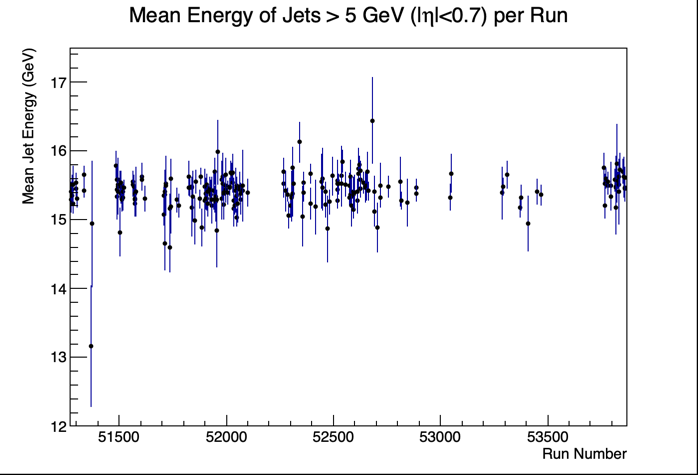
\includegraphics[width=\linewidth, trim=10 10 10 0, clip]{Figures/QA_Study/avg_ejet_case7.png}
        \caption{Average jet energy per event for triggers 16–23 and 32–35 under the same conditions.}
        \label{fig:avgEjet_case7}
    \end{subfigure}
    \caption{Jet QA observables under tightened leading jet threshold and relaxed azimuthal condition, for triggers 16–23 and 32–35.}
    \label{fig:qa_jet_summary_7}
\end{figure}

\begin{figure}[H]
    \centering
    \begin{subfigure}[t]{0.48\textwidth}
        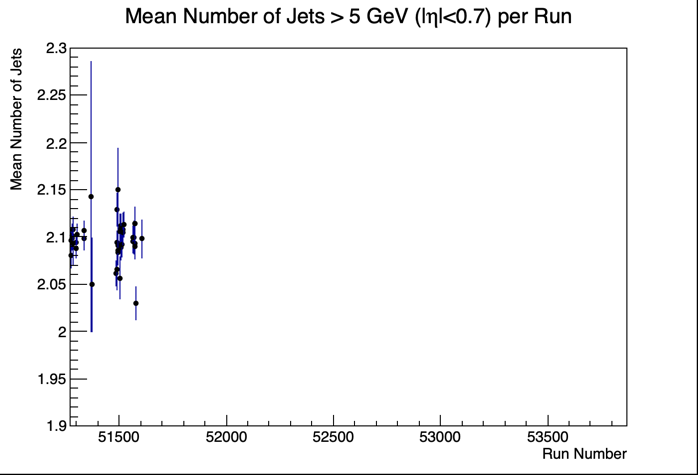
\includegraphics[width=\linewidth, trim=10 10 10 0, clip]{Figures/QA_Study/avg_njet_case8.png}
        \caption{Average number of jets per event for trigger 18 with \(p_T^{\text{lead}} > 15~\mathrm{GeV}/c\).}
        \label{fig:avgNjet_case8}
    \end{subfigure}
    \hfill
    \begin{subfigure}[t]{0.48\textwidth}
        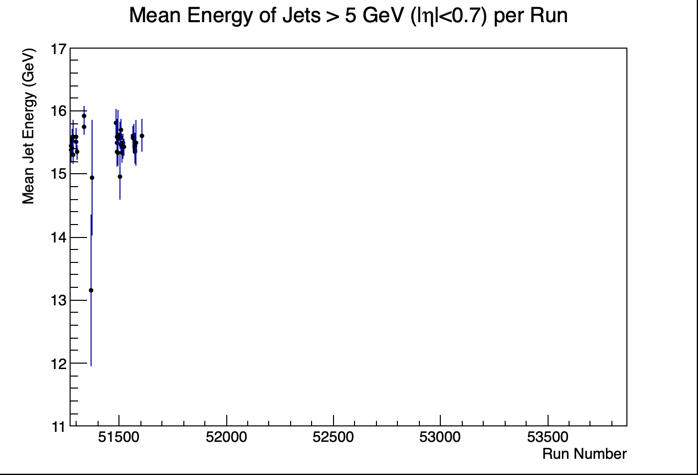
\includegraphics[width=\linewidth, trim=10 10 10 0, clip]{Figures/QA_Study/avg_ejet_case8.png}
        \caption{Average jet energy per event for trigger 18 under the same selection.}
        \label{fig:avgEjet_case8}
    \end{subfigure}
    \caption{Jet QA observables for trigger 18 under high \(p_T^{\text{lead}}\) and relaxed \(\Delta\phi\) conditions.}
    \label{fig:qa_jet_summary_8}
\end{figure}

\begin{figure}[H]
    \centering
    \begin{subfigure}[t]{0.48\textwidth}
        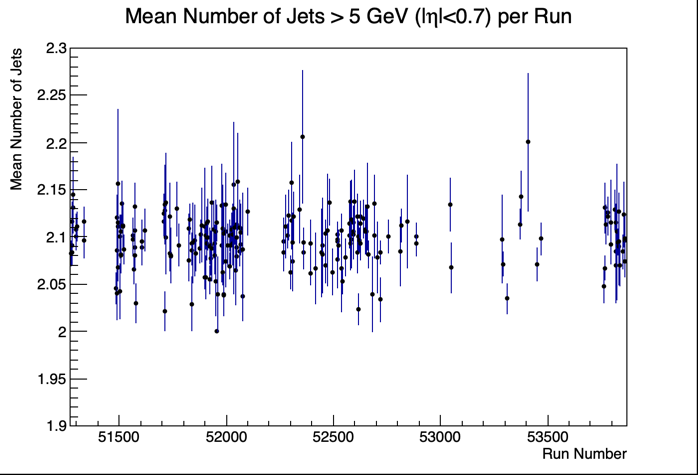
\includegraphics[width=\linewidth, trim=10 10 10 0, clip]{Figures/QA_Study/avg_njet_case9.png}
        \caption{Average number of jets per event for trigger 34 with high-\(p_T\) and relaxed angular selection.}
        \label{fig:avgNjet_case9}
    \end{subfigure}
    \hfill
    \begin{subfigure}[t]{0.48\textwidth}
        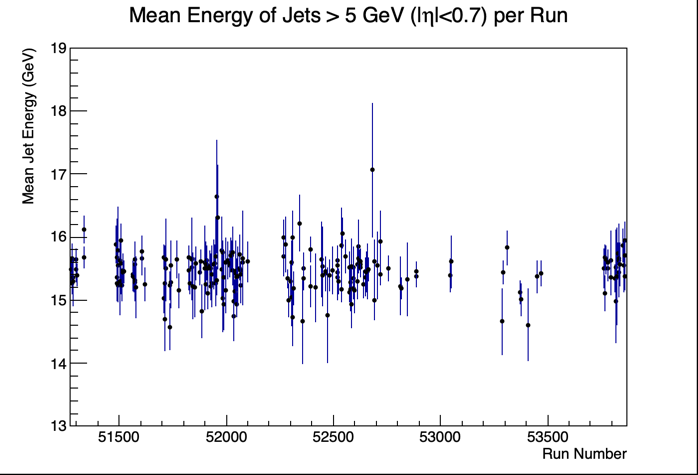
\includegraphics[width=\linewidth, trim=10 10 10 0, clip]{Figures/QA_Study/avg_ejet_case9.png}
        \caption{Average jet energy per event for trigger 34 under same conditions.}
        \label{fig:avgEjet_case9}
    \end{subfigure}
    \caption{Jet QA observables for trigger 34 with \(p_T^{\text{lead}} > 15~\mathrm{GeV}/c\), relaxed \(\Delta\phi\), and scaled subleading jet \(p_T\).}
    \label{fig:qa_jet_summary_9}
\end{figure}
To evaluate the stability and quality of the EMCal response during data-taking, a performance study was conducted for events triggered with IDs 16–23. The analysis focused on two main aspects: the average transverse energy (TE) in the transverse region—commonly associated with underlying event activity—and the status of EMCal towers over different run numbers.

Figure~\ref{fig:emcal_avgTE} shows the average transverse energy per event as a function of run number. This observable serves as a proxy for the level of underlying event activity and provides a consistency check across runs. The average TE remains stable over time, with minor fluctuations attributable to expected run-to-run variation.

To further ensure calorimeter quality, the fraction of hot and dead towers was monitored. As shown in Figure~\ref{fig:hot_towers}, most runs exhibit a negligible percentage of hot towers, except for run 51576, where approximately 17\% of towers are flagged as hot. This run was excluded from subsequent analyses to prevent bias in energy measurements.

The dead tower fraction is plotted in Figure~\ref{fig:dead_towers}, and the combined percentage of hot and dead towers is summarized in Figure~\ref{fig:total_bad_towers}. This confirms that run 51576 is the only outlier, with the rest of the dataset showing excellent calorimeter health.

Finally, Figure~\ref{fig:emcal_2D} presents a 2D correlation between the average TE and the percentage of problematic towers (hot or dead), further supporting the conclusion that the calorimeter performance is stable across the dataset, with the exception of the excluded run.

\begin{figure}[H]
    \centering
    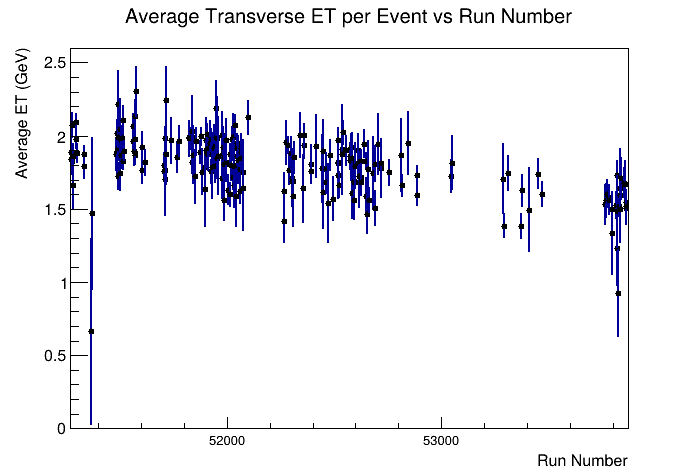
\includegraphics[width=0.5\linewidth]{Figures/QA_Study/avg_TE_vs_run.png}
    \caption{Average transverse energy (TE) per event in the transverse region as a function of run number for triggers 16–23.}
    \label{fig:emcal_avgTE}
\end{figure}

\begin{figure}[H]
    \centering
    \begin{subfigure}[t]{0.32\linewidth}
        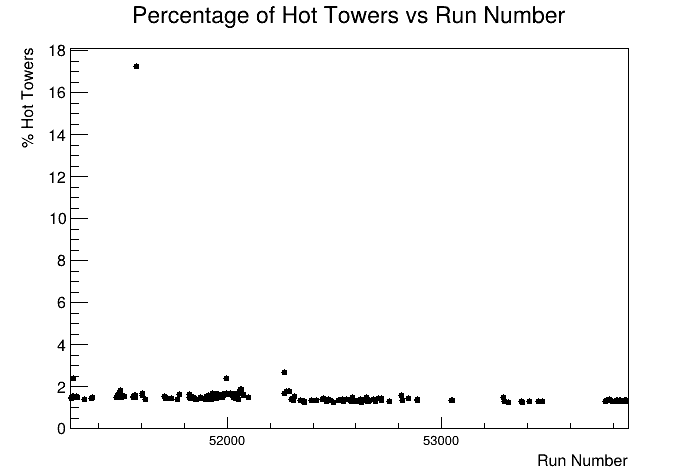
\includegraphics[width=\linewidth]{Figures/QA_Study/hot_towers_vs_run.png}
        \caption{Hot towers (\%)}
        \label{fig:hot_towers}
    \end{subfigure}
    \hfill
    \begin{subfigure}[t]{0.32\linewidth}
        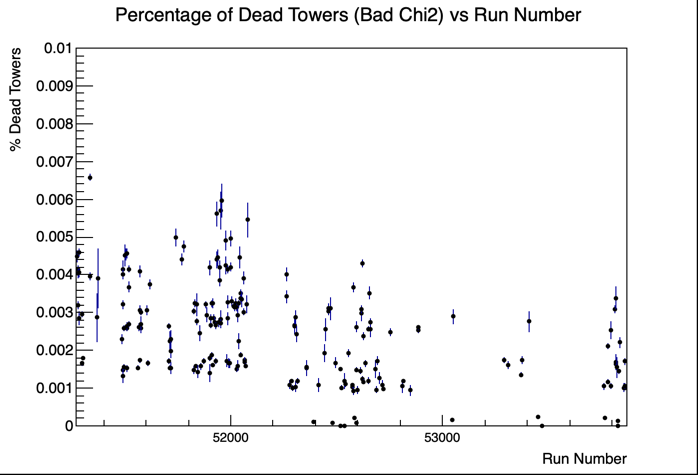
\includegraphics[width=\linewidth, trim=10 10 10 0, clip]{Figures/QA_Study/dead_towers_vs_run.png}
        \caption{Dead towers (\%)}
        \label{fig:dead_towers}
    \end{subfigure}
    \hfill
    \begin{subfigure}[t]{0.32\linewidth}
        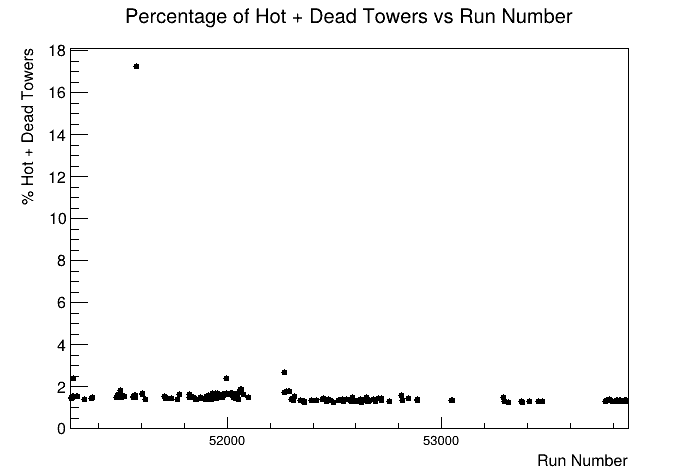
\includegraphics[width=\linewidth]{Figures/QA_Study/total_bad_towers_vs_run.png}
        \caption{Hot + Dead towers (\%)}
        \label{fig:total_bad_towers}
    \end{subfigure}
    \caption{Percentage of hot, dead, and total (hot + dead) EMCal towers versus run number.}
    \label{fig:emcal_bad_towers_summary}
\end{figure}



\begin{figure}[H]
    \centering
    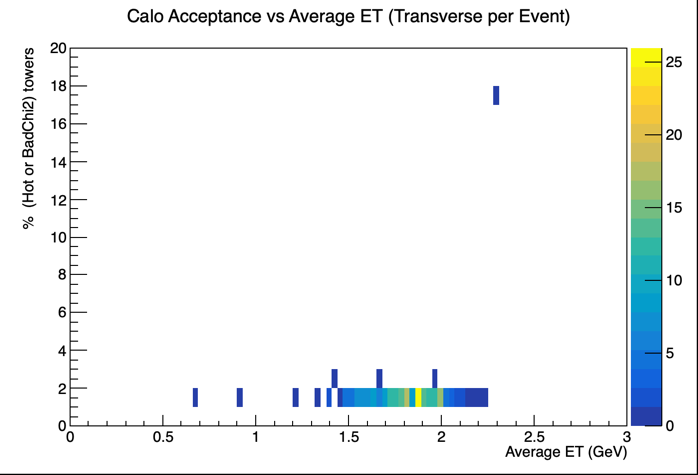
\includegraphics[width=0.5\linewidth, trim=10 10 10 0, clip]{Figures/QA_Study/2D_hot_dead_vs_avgTE.png}
    \caption{2D correlation of average transverse energy per event with the percentage of hot or dead towers, validating EMCal stability across the dataset.}
    \label{fig:emcal_2D}
\end{figure}

To assess calorimeter performance and underlying event activity, we measured the average transverse energy (\(E_T\)) per event in the electromagnetic calorimeter (EMCal), inner hadronic calorimeter (IHCal), and outer hadronic calorimeter (OHCal), using three azimuthal regions defined with respect to the leading jet direction: towards, transverse, and away. This study was conducted for events triggered by IDs 16–23, with a selection requiring the leading jet to have \(p_T^{\text{lead}} \geq 12~\mathrm{GeV}/c\) and the subleading jet to satisfy \(p_T^{\text{sublead}} \geq 7~\mathrm{GeV}/c\).

In the EMCal, the average transverse energy per event is approximately \(13~\mathrm{GeV}\) in the towards region, \(2~\mathrm{GeV}\) in the transverse region, and \(10.5~\mathrm{GeV}\) in the away region. These values are consistent with expectations based on jet topology and calorimeter response, with some fluctuations attributed to differences in the number of events collected across runs.

For the IHCal, the corresponding average \(E_T\) values are around \(1~\mathrm{GeV}\) in the towards region, \(0.2~\mathrm{GeV}\) in the transverse region, and \(1.2~\mathrm{GeV}\) in the away region, reflecting the generally lower energy deposits in the inner hadronic calorimeter.

The OHCal exhibits higher energy deposits compared to the IHCal, with average transverse energy values of approximately \(4.8~\mathrm{GeV}\) in both the towards and away regions, and about \(0.5~\mathrm{GeV}\) in the transverse region.

Figures~\ref{fig:emcal_et_regions}, \ref{fig:ihcal_et_regions}, and \ref{fig:ohcal_et_regions} show the run-by-run distributions of average transverse energy for the EMCal, IHCal, and OHCal, respectively, across the three jet-relative regions.

\begin{figure}[H]
    \centering
    \begin{subfigure}[t]{0.32\linewidth}
        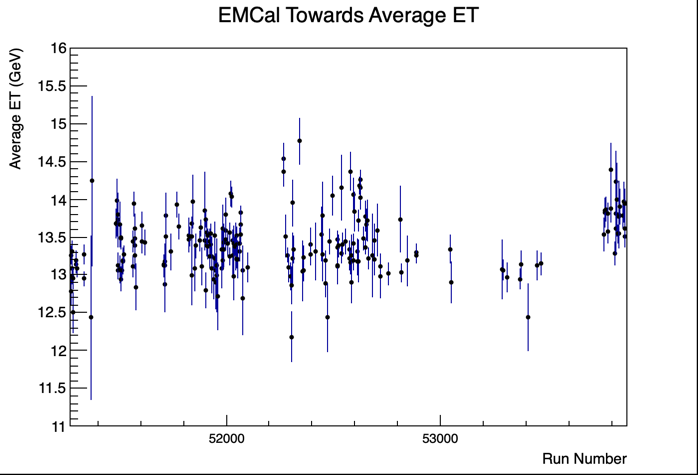
\includegraphics[width=\linewidth, trim=10 10 10 0, clip]{Figures/QA_Study/emcal_towards.png}
        \caption{EMCal: Towards region}
    \end{subfigure}
    \hfill
    \begin{subfigure}[t]{0.32\linewidth}
        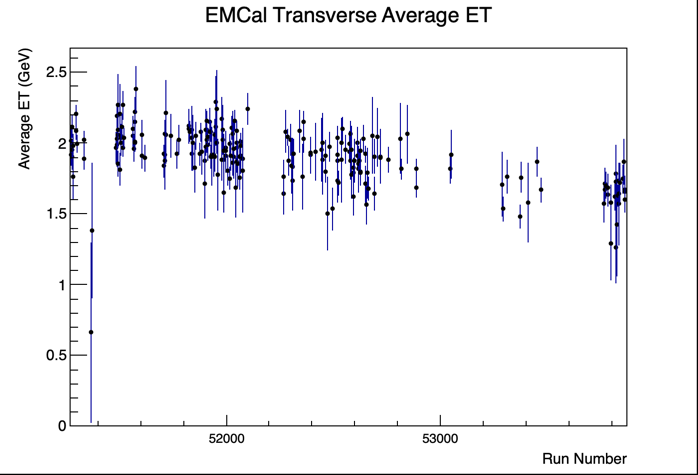
\includegraphics[width=\linewidth, trim=10 10 10 0, clip]{Figures/QA_Study/emcal_transverse.png}
        \caption{EMCal: Transverse region}
    \end{subfigure}
    \hfill
    \begin{subfigure}[t]{0.32\linewidth}
        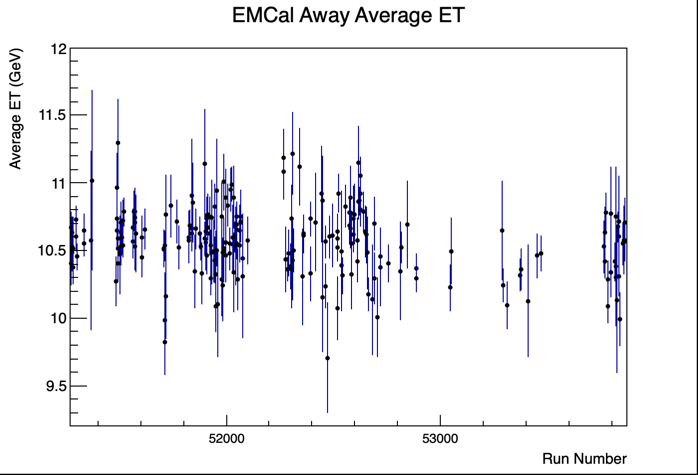
\includegraphics[width=\linewidth, trim=10 10 10 0, clip]{Figures/QA_Study/emcal_away.png}
        \caption{EMCal: Away region}
    \end{subfigure}
    \caption{Average transverse energy in EMCal per run, in the towards, transverse, and away regions.}
    \label{fig:emcal_et_regions}
\end{figure}

\begin{figure}[H]
    \centering
    \begin{subfigure}[t]{0.32\linewidth}
        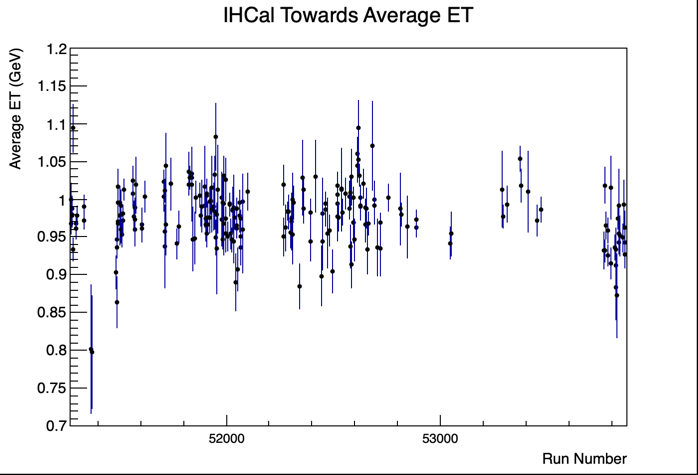
\includegraphics[width=\linewidth, trim=10 10 10 0, clip]{Figures/QA_Study/ihcal_towards.png}
        \caption{IHCal: Towards region}
    \end{subfigure}
    \hfill
    \begin{subfigure}[t]{0.32\linewidth}
        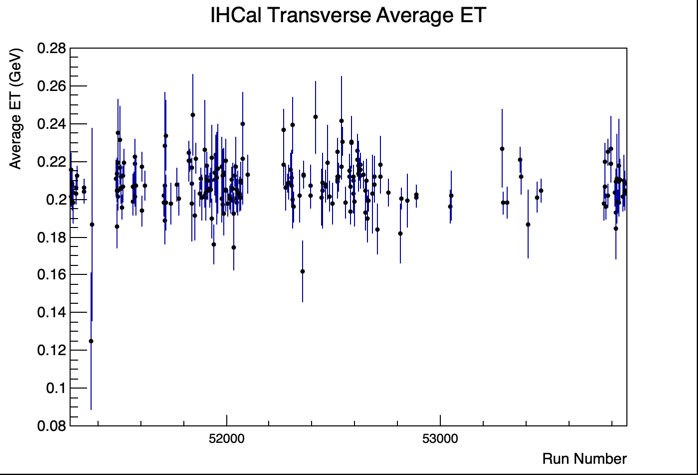
\includegraphics[width=\linewidth, trim=10 10 10 0, clip]{Figures/QA_Study/ihcal_transverse.png}
        \caption{IHCal: Transverse region}
    \end{subfigure}
    \hfill
    \begin{subfigure}[t]{0.32\linewidth}
        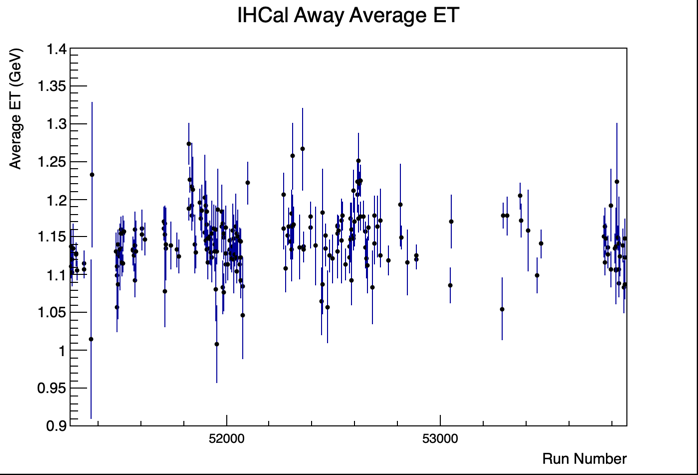
\includegraphics[width=\linewidth, trim=10 10 10 0, clip]{Figures/QA_Study/ihcal_away.png}
        \caption{IHCal: Away region}
    \end{subfigure}
    \caption{Average transverse energy in IHCal per run, in the towards, transverse, and away regions.}
    \label{fig:ihcal_et_regions}
\end{figure}

\begin{figure}[H]
    \centering
    \begin{subfigure}[t]{0.32\linewidth}
        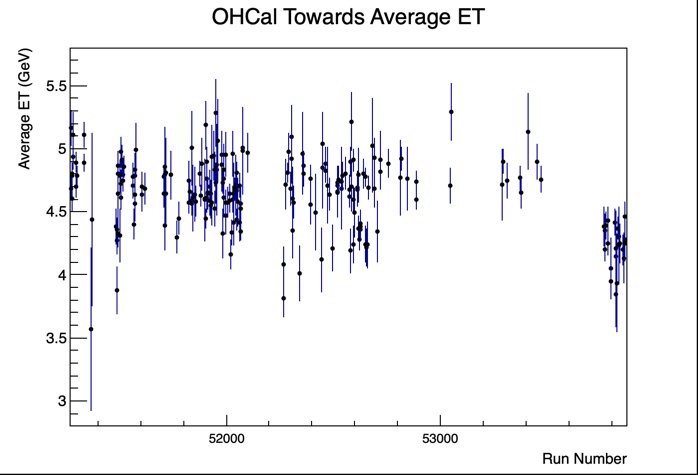
\includegraphics[width=\linewidth, trim=10 10 10 0, clip]{Figures/QA_Study/ohcal_towards.png}
        \caption{OHCal: Towards region}
    \end{subfigure}
    \hfill
    \begin{subfigure}[t]{0.32\linewidth}
        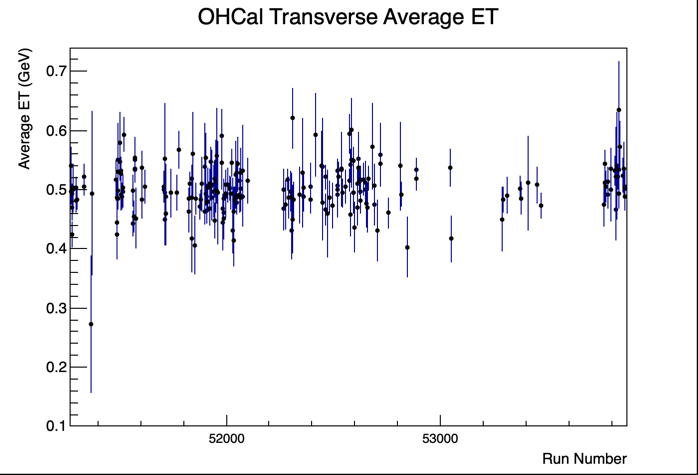
\includegraphics[width=\linewidth, trim=10 10 10 0, clip]{Figures/QA_Study/ohcal_transverse.png}
        \caption{OHCal: Transverse region}
    \end{subfigure}
    \hfill
    \begin{subfigure}[t]{0.32\linewidth}
        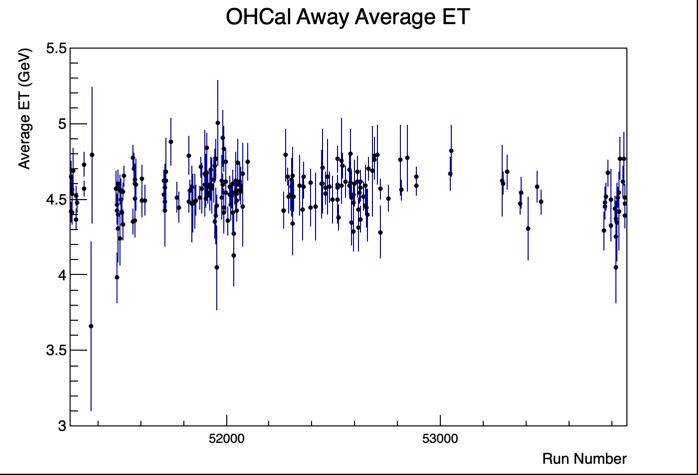
\includegraphics[width=\linewidth, trim=10 10 10 0, clip]{Figures/QA_Study/ohcal_away.png}
        \caption{OHCal: Away region}
    \end{subfigure}
    \caption{Average transverse energy in OHCal per run, in the towards, transverse, and away regions.}
    \label{fig:ohcal_et_regions}
\end{figure}

To evaluate the calorimeter response under extended trigger coverage, the average transverse energy (\(E_T\)) per event was studied in the EMCal, IHCal, and OHCal for events selected with trigger IDs 16–23 and 32–35. The selection criteria required the leading jet to have \(p_T^{\text{lead}} > 12~\mathrm{GeV}/c\), while the subleading jet was required to satisfy \(p_T^{\text{sublead}} > 0.3 \times p_T^{\text{lead}}\). The \(E_T\) distributions were evaluated in three azimuthal regions with respect to the leading jet axis: towards, transverse, and away.

In the EMCal, the average transverse energy was found to be approximately \(13~\mathrm{GeV}\) in the towards region, \(2~\mathrm{GeV}\) in the transverse region, and \(10~\mathrm{GeV}\) in the away region. These results are consistent with expectations for jet fragmentation and underlying event contributions. For the IHCal, the average transverse energy measured was about \(0.9~\mathrm{GeV}\) in the towards region, \(0.2~\mathrm{GeV}\) in the transverse region, and \(1.1~\mathrm{GeV}\) in the away region. In the OHCal, the corresponding values were approximately \(4.6~\mathrm{GeV}\), \(0.5~\mathrm{GeV}\), and \(4.1~\mathrm{GeV}\) for the towards, transverse, and away regions, respectively.

These measurements demonstrate consistency with previous observations and confirm the expected calorimetric behavior in the extended trigger range. The observed variation in transverse energy across runs remains within acceptable bounds and is attributed to fluctuations in event statistics and detector conditions.

\begin{figure}[H]
    \centering
    \begin{subfigure}[t]{0.32\linewidth}
        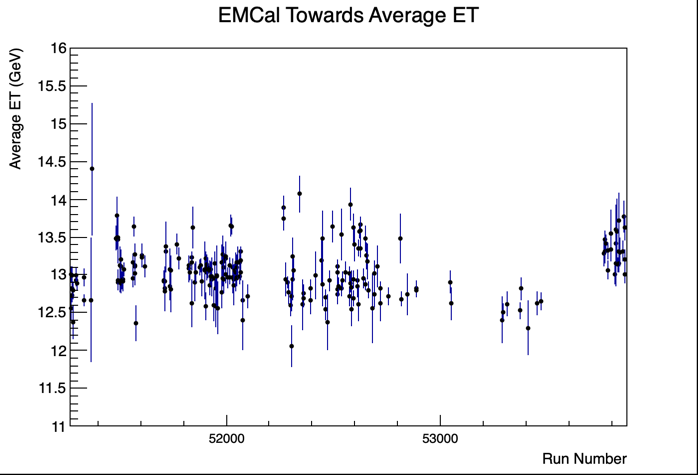
\includegraphics[width=\linewidth, trim=10 10 10 0, clip]{Figures/QA_Study/emcal_towards_case2.png}
        \caption{EMCal: Towards region}
    \end{subfigure}
    \hfill
    \begin{subfigure}[t]{0.32\linewidth}
        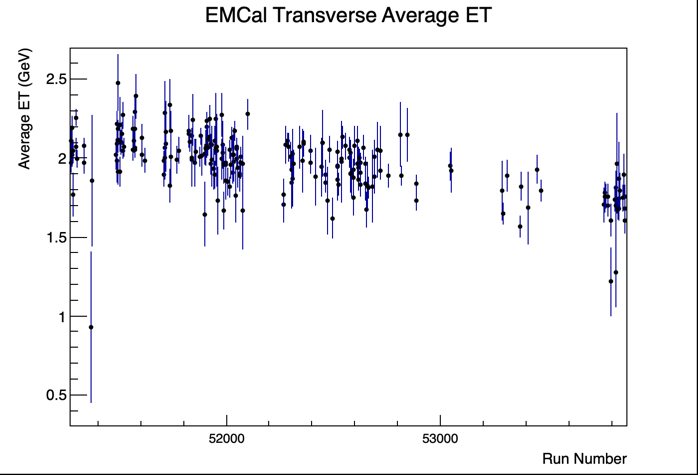
\includegraphics[width=\linewidth, trim=10 10 10 0, clip]{Figures/QA_Study/emcal_transverse_case2.png}
        \caption{EMCal: Transverse region}
    \end{subfigure}
    \hfill
    \begin{subfigure}[t]{0.32\linewidth}
        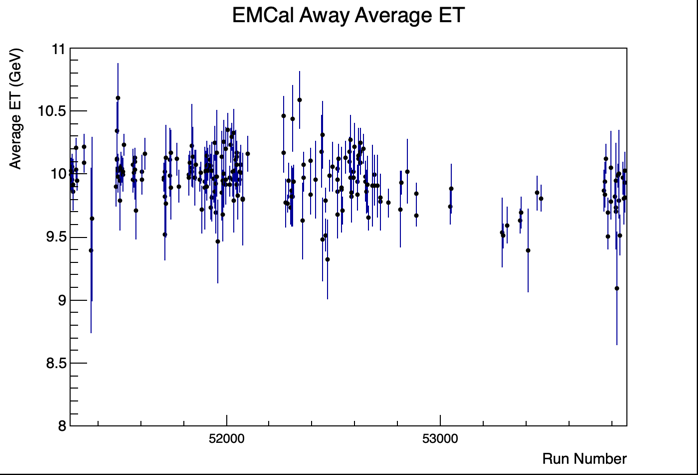
\includegraphics[width=\linewidth, trim=10 10 10 0, clip]{Figures/QA_Study/emcal_away_case2.png}
        \caption{EMCal: Away region}
    \end{subfigure}
    \caption{Average transverse energy in EMCal per run for triggers 16–23 and 32–35, in the towards, transverse, and away regions.}
    \label{fig:emcal_et_regions_case2}
\end{figure}

\begin{figure}[H]
    \centering
    \begin{subfigure}[t]{0.32\linewidth}
        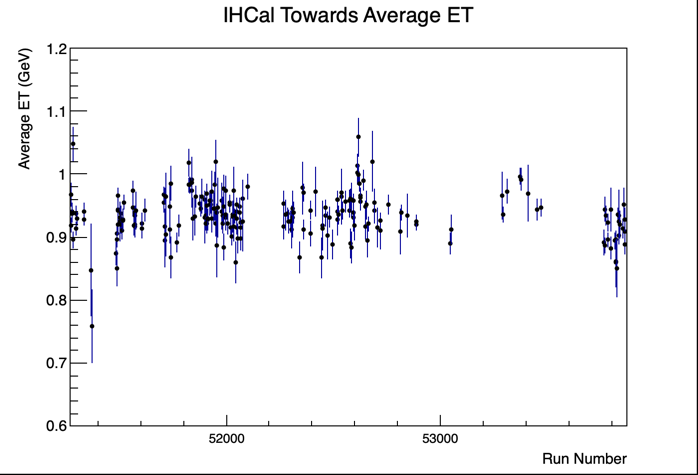
\includegraphics[width=\linewidth, trim=10 10 10 0, clip]{Figures/QA_Study/ihcal_towards_case2.png}
        \caption{IHCal: Towards region}
    \end{subfigure}
    \hfill
    \begin{subfigure}[t]{0.32\linewidth}
        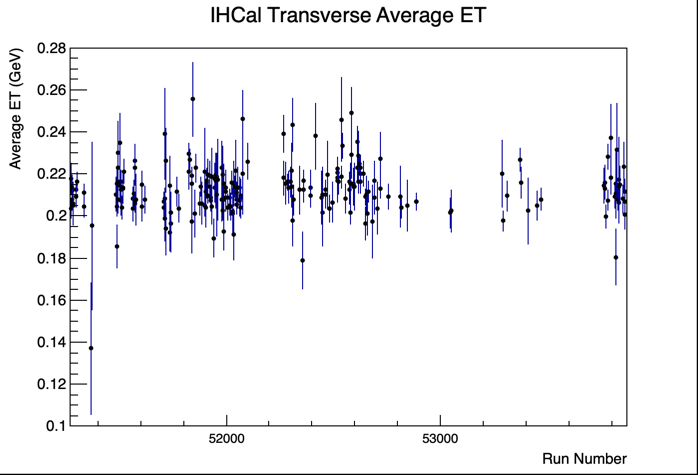
\includegraphics[width=\linewidth, trim=10 10 10 0, clip]{Figures/QA_Study/ihcal_transverse_case2.png}
        \caption{IHCal: Transverse region}
    \end{subfigure}
    \hfill
    \begin{subfigure}[t]{0.32\linewidth}
        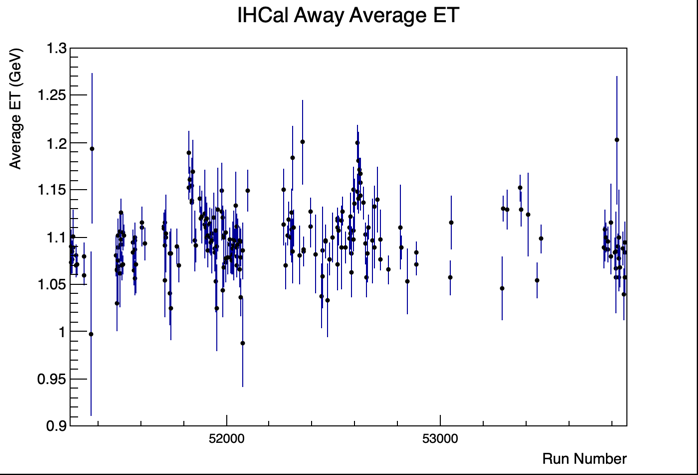
\includegraphics[width=\linewidth, trim=10 10 10 0, clip]{Figures/QA_Study/ihcal_away_case2.png}
        \caption{IHCal: Away region}
    \end{subfigure}
    \caption{Average transverse energy in IHCal per run for triggers 16–23 and 32–35, in the towards, transverse, and away regions.}
    \label{fig:ihcal_et_regions_case2}
\end{figure}

\begin{figure}[H]
    \centering
    \begin{subfigure}[t]{0.32\linewidth}
        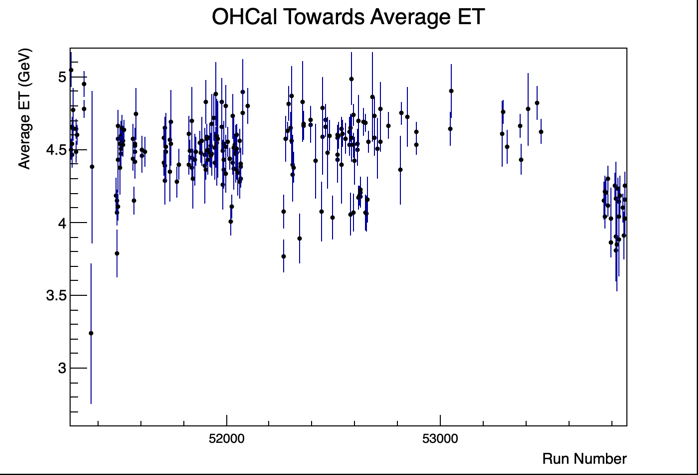
\includegraphics[width=\linewidth, trim=10 10 10 0, clip]{Figures/QA_Study/ohcal_towards_case2.png}
        \caption{OHCal: Towards region}
    \end{subfigure}
    \hfill
    \begin{subfigure}[t]{0.32\linewidth}
        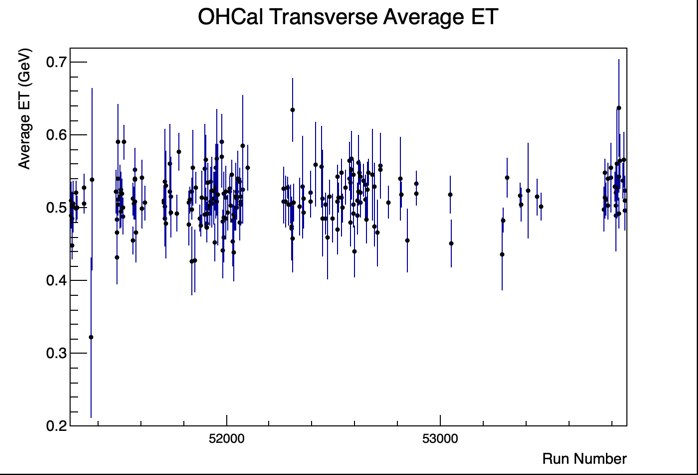
\includegraphics[width=\linewidth, trim=10 10 10 0, clip]{Figures/QA_Study/ohcal_transverse_case2.png}
        \caption{OHCal: Transverse region}
    \end{subfigure}
    \hfill
    \begin{subfigure}[t]{0.32\linewidth}
        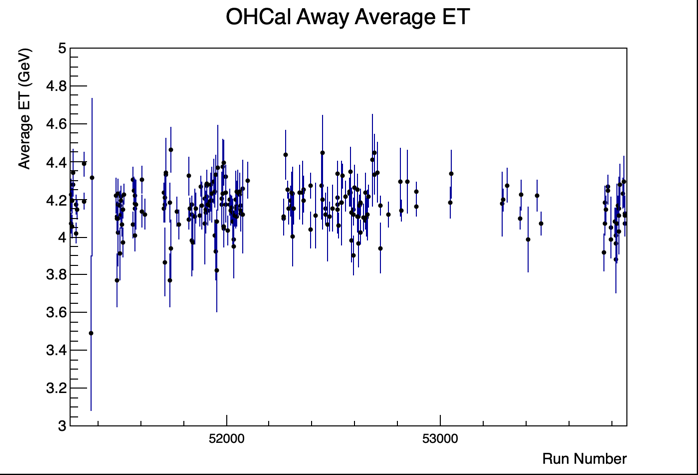
\includegraphics[width=\linewidth, trim=10 10 10 0, clip]{Figures/QA_Study/ohcal_away_case2.png}
        \caption{OHCal: Away region}
    \end{subfigure}
    \caption{Average transverse energy in OHCal per run for triggers 16–23 and 32–35, in the towards, transverse, and away regions.}
    \label{fig:ohcal_et_regions_case2}
\end{figure}

To assess the calorimeter performance under trigger 18 selection, the average transverse energy (\(E_T\)) per event was measured in the EMCal, IHCal, and OHCal across three azimuthal regions: towards, transverse, and away. Events were required to have a leading jet with \(p_T^{\text{lead}} > 12~\mathrm{GeV}/c\), and a subleading jet satisfying \(p_T^{\text{sublead}} > 0.3 \times p_T^{\text{lead}}\). This selection ensures that both jets have significant transverse momentum, enabling a meaningful study of jet-related energy deposition and underlying event activity.

In the EMCal, the average transverse energy was found to be approximately \(13~\mathrm{GeV}\) in the towards region, \(2~\mathrm{GeV}\) in the transverse region, and \(10~\mathrm{GeV}\) in the away region. For the IHCal, the average \(E_T\) was around \(0.9~\mathrm{GeV}\) in the towards region, \(0.2~\mathrm{GeV}\) in the transverse region, and \(1.1~\mathrm{GeV}\) in the away region. The OHCal measurements showed average transverse energies of about \(4.6~\mathrm{GeV}\), \(0.5~\mathrm{GeV}\), and \(4.1~\mathrm{GeV}\) in the towards, transverse, and away regions, respectively.

These results are consistent with prior observations from other trigger selections and support the stability of the calorimeter response across different trigger configurations. Minor variations in energy values across runs are attributed to fluctuations in the number of recorded events and inherent run-to-run differences.

\begin{figure}[H]
    \centering
    \begin{subfigure}[t]{0.32\linewidth}
        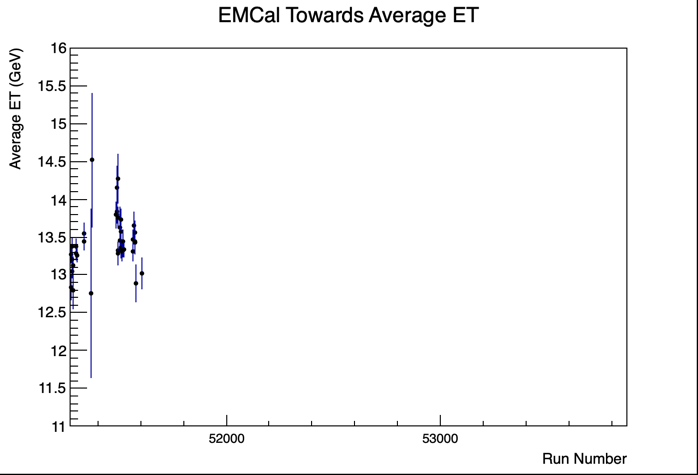
\includegraphics[width=\linewidth, trim=10 10 10 0, clip]{Figures/QA_Study/emcal_towards_case3.png}
        \caption{EMCal: Towards region}
    \end{subfigure}
    \hfill
    \begin{subfigure}[t]{0.32\linewidth}
        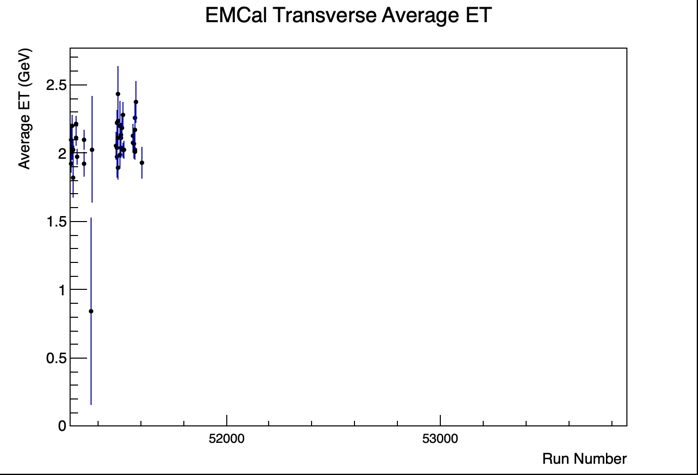
\includegraphics[width=\linewidth, trim=10 10 10 0, clip]{Figures/QA_Study/emcal_transverse_case3.png}
        \caption{EMCal: Transverse region}
    \end{subfigure}
    \hfill
    \begin{subfigure}[t]{0.32\linewidth}
        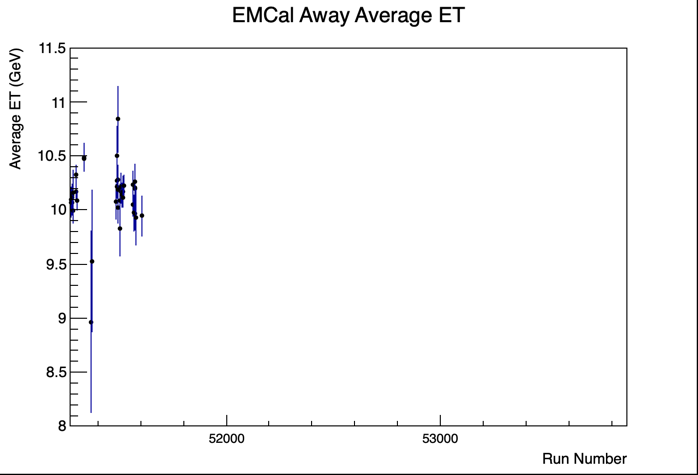
\includegraphics[width=\linewidth, trim=10 10 10 0, clip]{Figures/QA_Study/emcal_away_case3.png}
        \caption{EMCal: Away region}
    \end{subfigure}
    \caption{Average transverse energy in EMCal per run for trigger 18, in the towards, transverse, and away regions.}
    \label{fig:emcal_et_regions_case3}
\end{figure}

\begin{figure}[H]
    \centering
    \begin{subfigure}[t]{0.32\linewidth}
        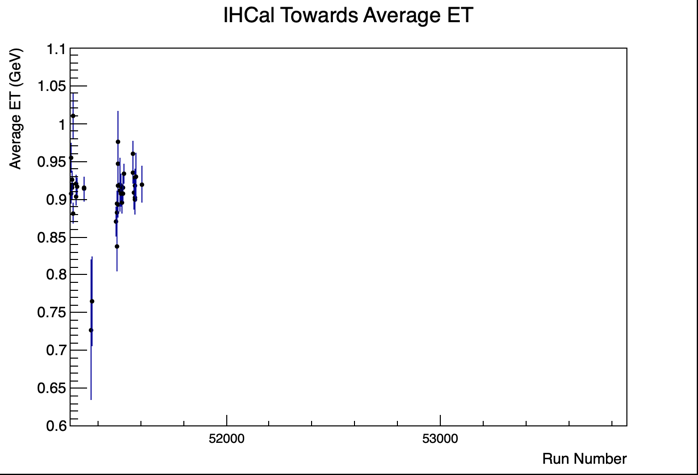
\includegraphics[width=\linewidth, trim=10 10 10 0, clip]{Figures/QA_Study/ihcal_towards_case3.png}
        \caption{IHCal: Towards region}
    \end{subfigure}
    \hfill
    \begin{subfigure}[t]{0.32\linewidth}
        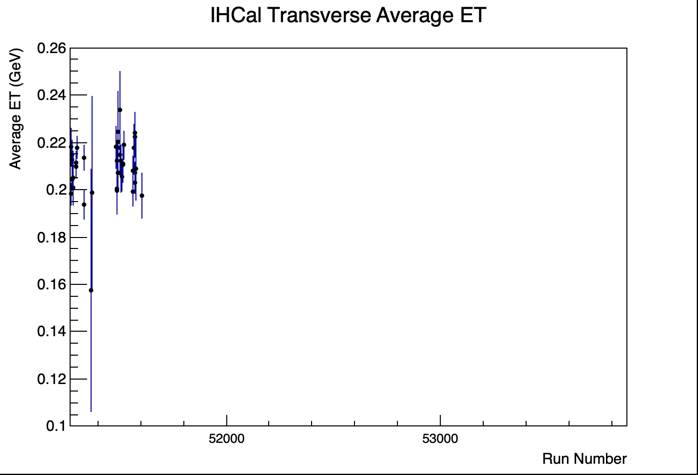
\includegraphics[width=\linewidth, trim=10 10 10 0, clip]{Figures/QA_Study/ihcal_transverse_case3.png}
        \caption{IHCal: Transverse region}
    \end{subfigure}
    \hfill
    \begin{subfigure}[t]{0.32\linewidth}
        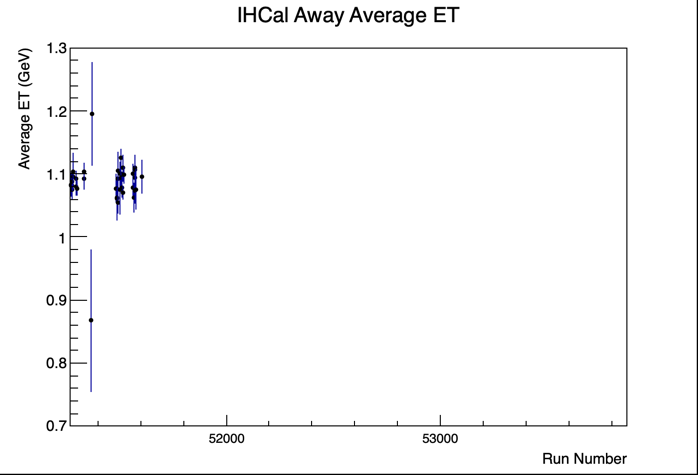
\includegraphics[width=\linewidth, trim=10 10 10 0, clip]{Figures/QA_Study/ihcal_away_case3.png}
        \caption{IHCal: Away region}
    \end{subfigure}
    \caption{Average transverse energy in IHCal per run for trigger 18, in the towards, transverse, and away regions.}
    \label{fig:ihcal_et_regions_case3}
\end{figure}

\begin{figure}[H]
    \centering
    \begin{subfigure}[t]{0.32\linewidth}
        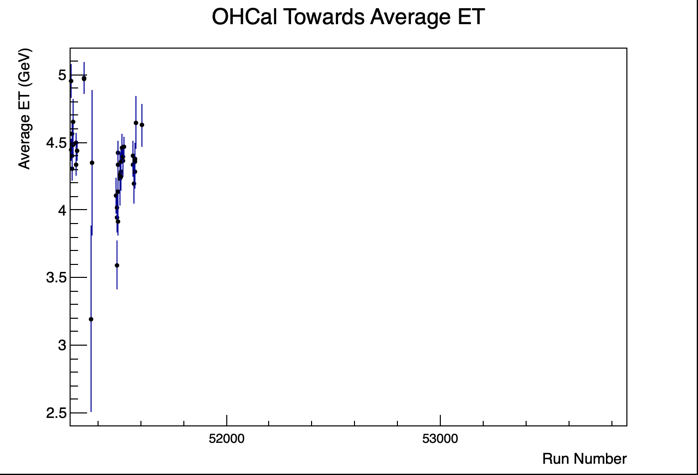
\includegraphics[width=\linewidth, trim=10 10 10 0, clip]{Figures/QA_Study/ohcal_towards_case3.png}
        \caption{OHCal: Towards region}
    \end{subfigure}
    \hfill
    \begin{subfigure}[t]{0.32\linewidth}
        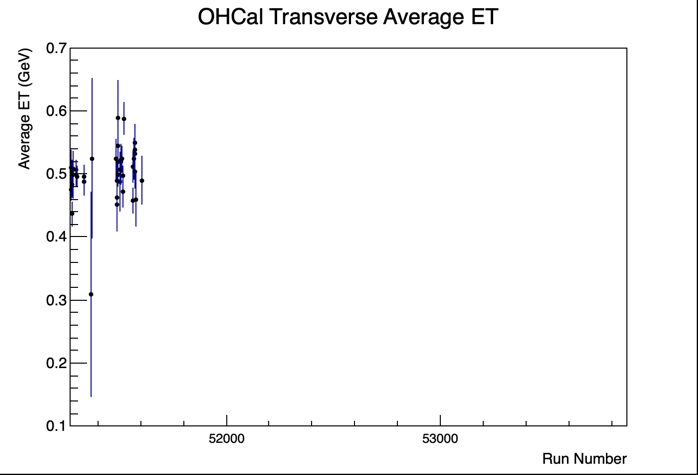
\includegraphics[width=\linewidth, trim=10 10 10 0, clip]{Figures/QA_Study/ohcal_transverse_case3.png}
        \caption{OHCal: Transverse region}
    \end{subfigure}
    \hfill
    \begin{subfigure}[t]{0.32\linewidth}
        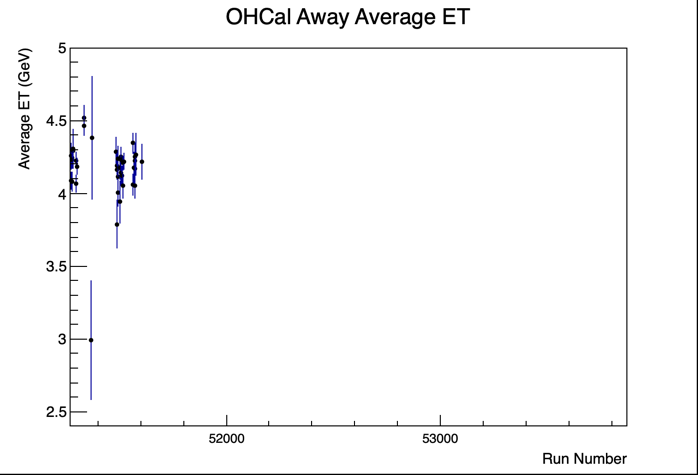
\includegraphics[width=\linewidth, trim=10 10 10 0, clip]{Figures/QA_Study/ohcal_away_case3.png}
        \caption{OHCal: Away region}
    \end{subfigure}
    \caption{Average transverse energy in OHCal per run for trigger 18, in the towards, transverse, and away regions.}
    \label{fig:ohcal_et_regions_case3}
\end{figure}


An additional set of transverse energy (\(E_T\)) measurements was performed for events selected with trigger 34, applying the same jet selection criteria as in previous studies: the leading jet is required to have \(p_T^{\text{lead}} > 12~\mathrm{GeV}/c\), and the subleading jet must satisfy \(p_T^{\text{sublead}} > 0.3 \times p_T^{\text{lead}}\). The measurements cover the EMCal, IHCal, and OHCal across the towards, transverse, and away azimuthal regions.

The results observed for trigger 34 are consistent with those from triggers 16–23 and 18. In the EMCal, the average transverse energy per event remains around \(13~\mathrm{GeV}\) in the towards region, \(2~\mathrm{GeV}\) in the transverse region, and \(10~\mathrm{GeV}\) in the away region. For the IHCal, the average \(E_T\) is approximately \(0.9~\mathrm{GeV}\), \(0.2~\mathrm{GeV}\), and \(1.1~\mathrm{GeV}\) for the towards, transverse, and away regions, respectively. The OHCal measurements yield approximately \(4.6~\mathrm{GeV}\) in the towards region, \(0.5~\mathrm{GeV}\) in the transverse region, and \(4.1~\mathrm{GeV}\) in the away region.

These findings further confirm the stability and reliability of the calorimeter system across different event selections and jet topologies, with no significant deviations observed under trigger 34.

\begin{figure}[H]
    \centering
    \begin{subfigure}[t]{0.32\linewidth}
        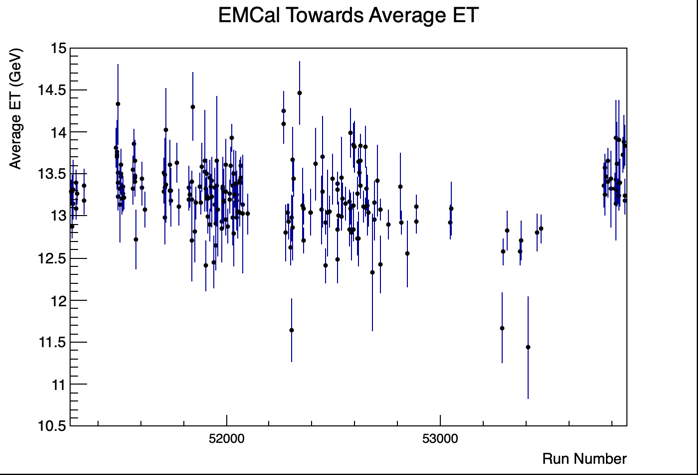
\includegraphics[width=\linewidth, trim=10 10 10 0, clip]{Figures/QA_Study/emcal_towards_case4.png}
        \caption{EMCal: Towards region}
    \end{subfigure}
    \hfill
    \begin{subfigure}[t]{0.32\linewidth}
        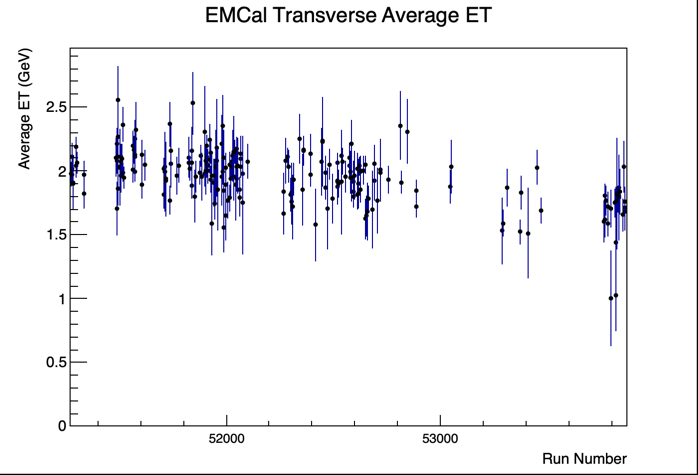
\includegraphics[width=\linewidth, trim=10 10 10 0, clip]{Figures/QA_Study/emcal_transverse_case4.png}
        \caption{EMCal: Transverse region}
    \end{subfigure}
    \hfill
    \begin{subfigure}[t]{0.32\linewidth}
        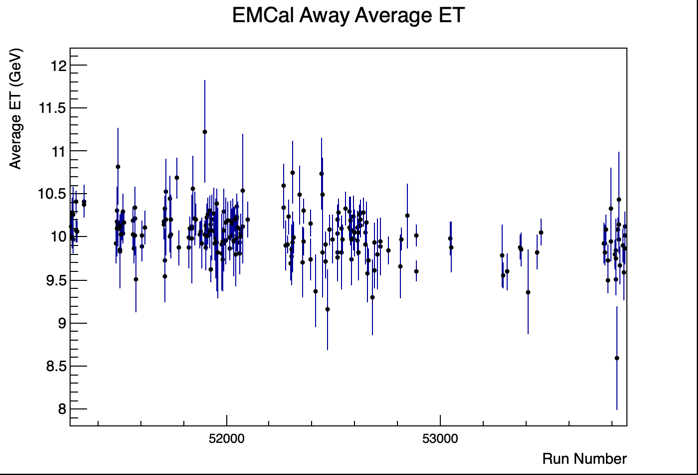
\includegraphics[width=\linewidth, trim=10 10 10 0, clip]{Figures/QA_Study/emcal_away_case4.png}
        \caption{EMCal: Away region}
    \end{subfigure}
    \caption{Average transverse energy in EMCal per run for trigger 34, in the towards, transverse, and away regions.}
    \label{fig:emcal_et_regions_case4}
\end{figure}

\begin{figure}[H]
    \centering
    \begin{subfigure}[t]{0.32\linewidth}
        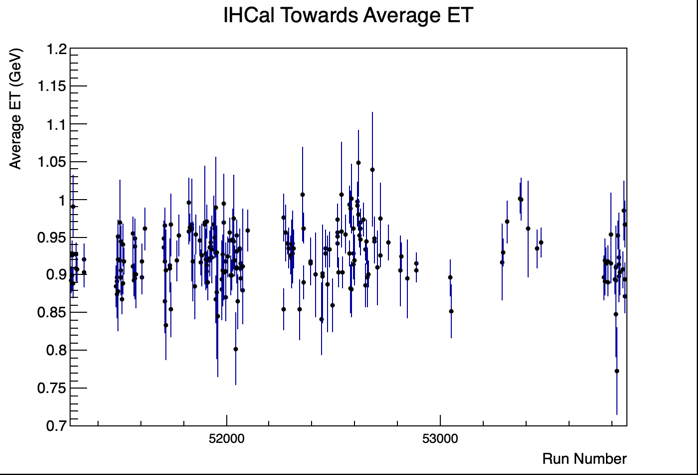
\includegraphics[width=\linewidth, trim=10 10 10 0, clip]{Figures/QA_Study/ihcal_towards_case4.png}
        \caption{IHCal: Towards region}
    \end{subfigure}
    \hfill
    \begin{subfigure}[t]{0.32\linewidth}
        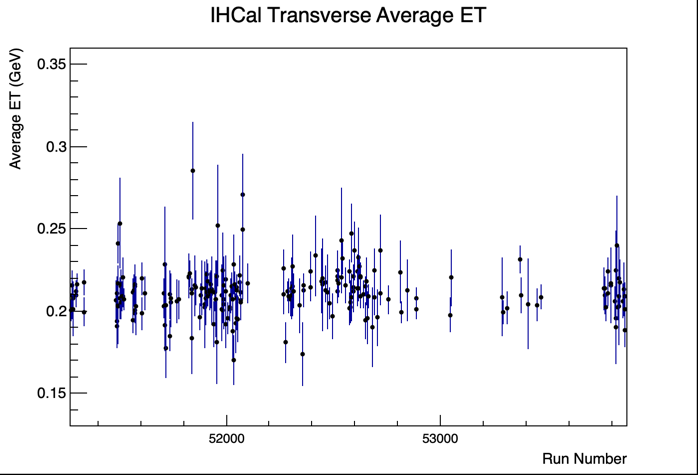
\includegraphics[width=\linewidth, trim=10 10 10 0, clip]{Figures/QA_Study/ihcal_transverse_case4.png}
        \caption{IHCal: Transverse region}
    \end{subfigure}
    \hfill
    \begin{subfigure}[t]{0.32\linewidth}
        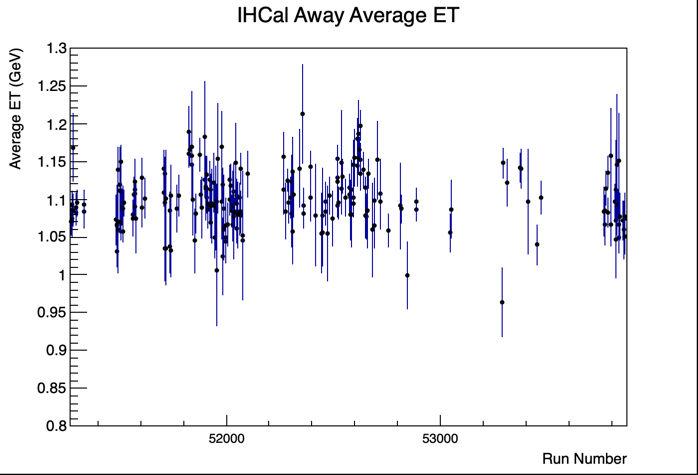
\includegraphics[width=\linewidth, trim=10 10 10 0, clip]{Figures/QA_Study/ihcal_away_case4.png}
        \caption{IHCal: Away region}
    \end{subfigure}
    \caption{Average transverse energy in IHCal per run for trigger 34, in the towards, transverse, and away regions.}
    \label{fig:ihcal_et_regions_case4}
\end{figure}

\begin{figure}[H]
    \centering
    \begin{subfigure}[t]{0.32\linewidth}
        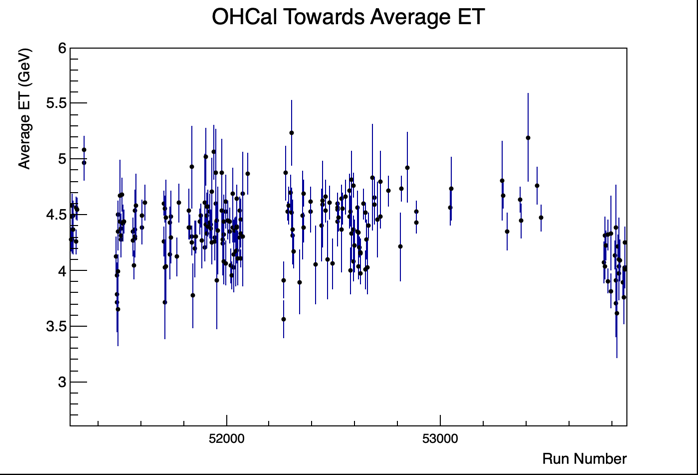
\includegraphics[width=\linewidth, trim=10 10 10 0, clip]{Figures/QA_Study/ohcal_towards_case4.png}
        \caption{OHCal: Towards region}
    \end{subfigure}
    \hfill
    \begin{subfigure}[t]{0.32\linewidth}
        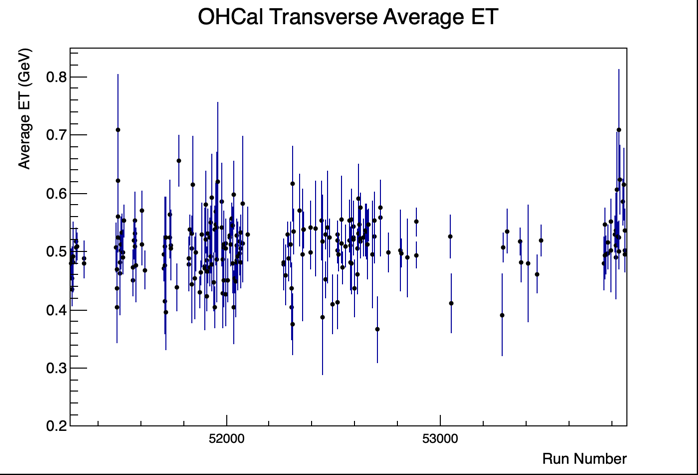
\includegraphics[width=\linewidth, trim=10 10 10 0, clip]{Figures/QA_Study/ohcal_transverse_case4.png}
        \caption{OHCal: Transverse region}
    \end{subfigure}
    \hfill
    \begin{subfigure}[t]{0.32\linewidth}
        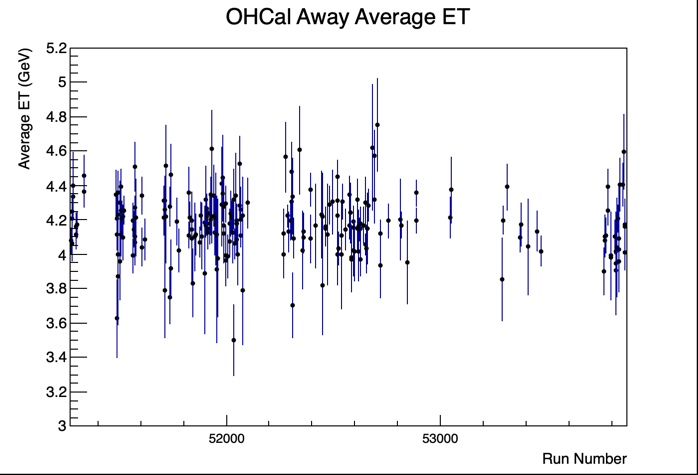
\includegraphics[width=\linewidth, trim=10 10 10 0, clip]{Figures/QA_Study/ohcal_away_case4.png}
        \caption{OHCal: Away region}
    \end{subfigure}
    \caption{Average transverse energy in OHCal per run for trigger 34, in the towards, transverse, and away regions.}
    \label{fig:ohcal_et_regions_case4}
\end{figure}
An extended study was conducted using a more stringent selection on the leading jet transverse momentum, requiring \(p_T^{\text{lead}} > 15~\mathrm{GeV}/c\), while maintaining the condition \(p_T^{\text{sublead}} > 0.3 \times p_T^{\text{lead}}\). Events from triggers 16–23 and 32–35 were analyzed to evaluate the calorimeter response in the towards, transverse, and away azimuthal regions.

In the EMCal, the average transverse energy per event is approximately \(15~\mathrm{GeV}\) in the towards region, \(2~\mathrm{GeV}\) in the transverse region, and \(11~\mathrm{GeV}\) in the away region. The IHCal shows average values of around \(1~\mathrm{GeV}\), \(0.2~\mathrm{GeV}\), and \(1.2~\mathrm{GeV}\) for the towards, transverse, and away regions, respectively. For the OHCal, the corresponding averages are approximately \(5.3~\mathrm{GeV}\), \(0.5~\mathrm{GeV}\), and \(5~\mathrm{GeV}\) in the towards, transverse, and away regions.

These results are in line with expectations, demonstrating a clear energy flow pattern across the detector and validating the stability of the calorimeter performance under tighter jet selection criteria.

\begin{figure}[H]
    \centering
    \begin{subfigure}[t]{0.32\textwidth}
        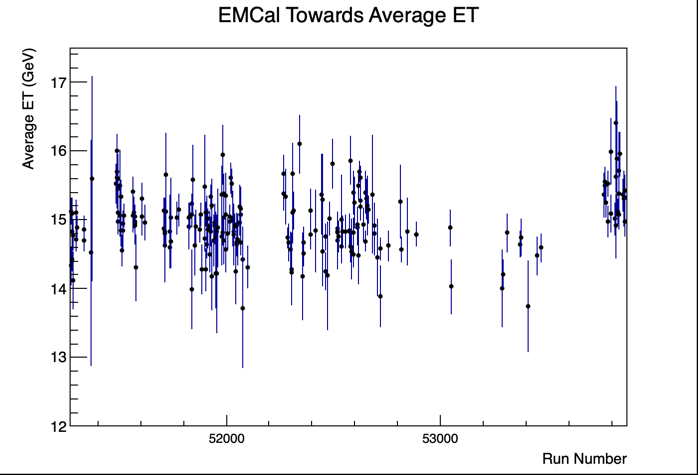
\includegraphics[width=\linewidth, trim=10 10 10 0, clip]{Figures/QA_Study/avg_et_emcal_towards_case5.png}
        \caption{EMCal: Towards region}
    \end{subfigure}
    \hfill
    \begin{subfigure}[t]{0.32\textwidth}
        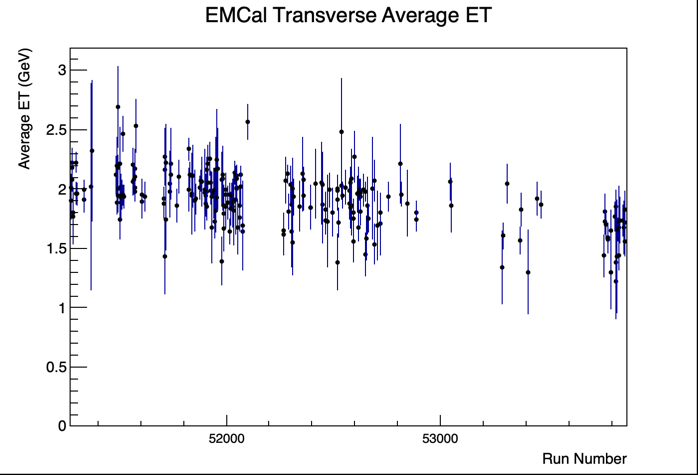
\includegraphics[width=\linewidth, trim=10 10 10 0, clip]{Figures/QA_Study/avg_et_emcal_transverse_case5.png}
        \caption{EMCal: Transverse region}
    \end{subfigure}
    \hfill
    \begin{subfigure}[t]{0.32\textwidth}
        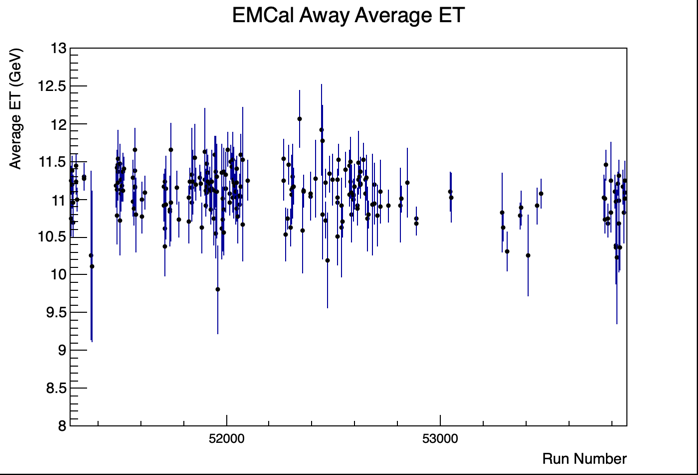
\includegraphics[width=\linewidth, trim=10 10 10 0, clip]{Figures/QA_Study/avg_et_emcal_away_case5.png}
        \caption{EMCal: Away region}
    \end{subfigure}
    \caption{Average transverse energy in EMCal for triggers 16–23 and 32–35 with \(p_T^{\text{lead}} > 15~\mathrm{GeV}/c\).}
    \label{fig:avg_et_emcal_case5}
\end{figure}

\begin{figure}[H]
    \centering
    \begin{subfigure}[t]{0.32\textwidth}
        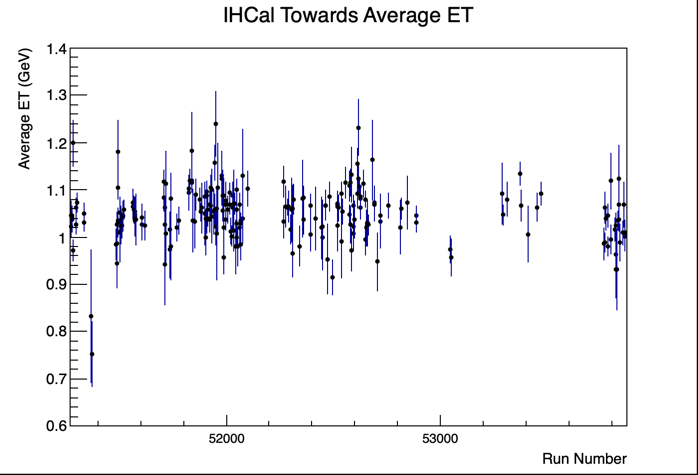
\includegraphics[width=\linewidth, trim=10 10 10 0, clip]{Figures/QA_Study/avg_et_ihcal_towards_case5.png}
        \caption{IHCal: Towards region}
    \end{subfigure}
    \hfill
    \begin{subfigure}[t]{0.32\textwidth}
        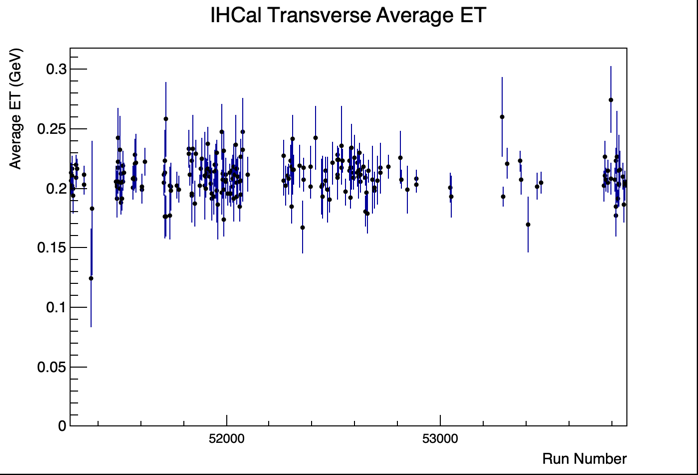
\includegraphics[width=\linewidth, trim=10 10 10 0, clip]{Figures/QA_Study/avg_et_ihcal_transverse_case5.png}
        \caption{IHCal: Transverse region}
    \end{subfigure}
    \hfill
    \begin{subfigure}[t]{0.32\textwidth}
        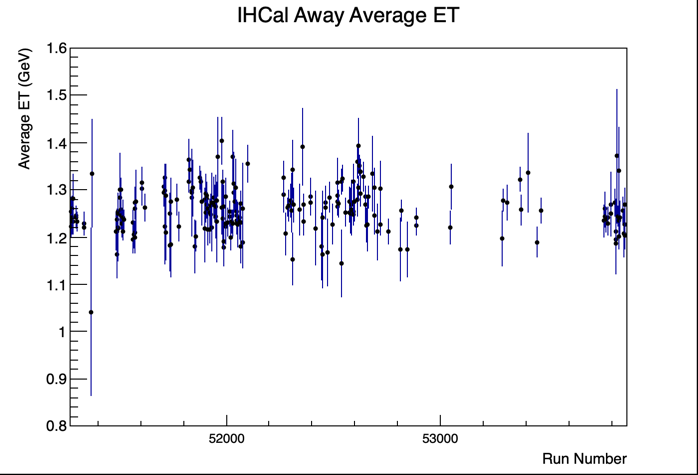
\includegraphics[width=\linewidth, trim=10 10 10 0, clip]{Figures/QA_Study/avg_et_ihcal_away_case5.png}
        \caption{IHCal: Away region}
    \end{subfigure}
    \caption{Average transverse energy in IHCal for triggers 16–23 and 32–35 with \(p_T^{\text{lead}} > 15~\mathrm{GeV}/c\).}
    \label{fig:avg_et_ihcal_case5}
\end{figure}

\begin{figure}[H]
    \centering
    \begin{subfigure}[t]{0.32\textwidth}
        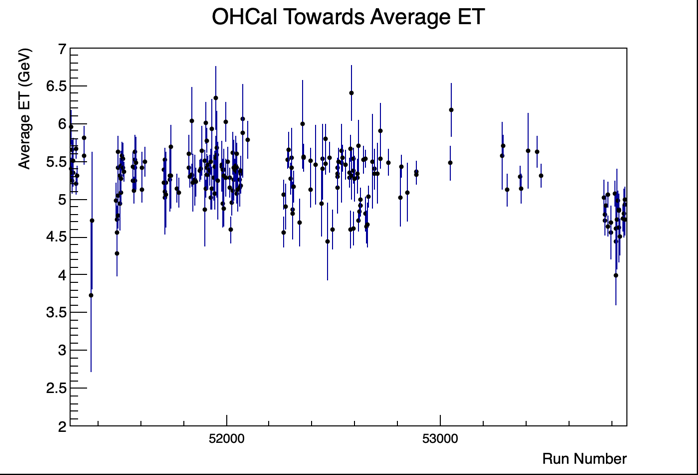
\includegraphics[width=\linewidth, trim=10 10 10 0, clip]{Figures/QA_Study/avg_et_ohcal_towards_case5.png}
        \caption{OHCal: Towards region}
    \end{subfigure}
    \hfill
    \begin{subfigure}[t]{0.32\textwidth}
        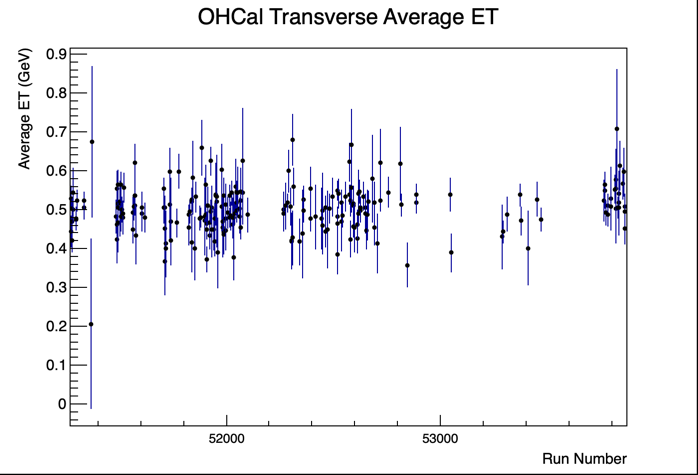
\includegraphics[width=\linewidth, trim=10 10 10 0, clip]{Figures/QA_Study/avg_et_ohcal_transverse_case5.png}
        \caption{OHCal: Transverse region}
    \end{subfigure}
    \hfill
    \begin{subfigure}[t]{0.32\textwidth}
        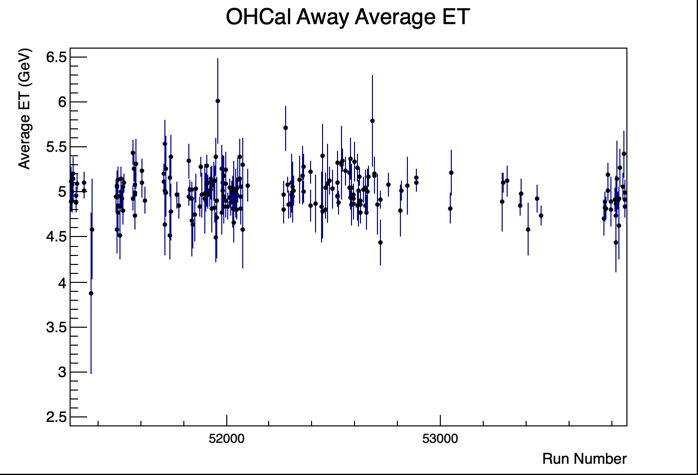
\includegraphics[width=\linewidth, trim=10 10 10 0, clip]{Figures/QA_Study/avg_et_ohcal_away_case5.png}
        \caption{OHCal: Away region}
    \end{subfigure}
    \caption{Average transverse energy in OHCal for triggers 16–23 and 32–35 with \(p_T^{\text{lead}} > 15~\mathrm{GeV}/c\).}
    \label{fig:avg_et_ohcal_case5}
\end{figure}

The average transverse energy was also evaluated for events selected with trigger 18 under the criteria \(p_T^{\text{lead}} > 15~\mathrm{GeV}/c\) and \(p_T^{\text{sublead}} > 0.3 \times p_T^{\text{lead}}\). The transverse energy was analyzed in the towards, transverse, and away regions of the EMCal, IHCal, and OHCal.

The results show consistency with previous observations: in the EMCal, the average transverse energy is approximately \(15~\mathrm{GeV}\) in the towards region, \(2~\mathrm{GeV}\) in the transverse region, and \(11~\mathrm{GeV}\) in the away region. For the IHCal, the corresponding values are \(1~\mathrm{GeV}\), \(0.2~\mathrm{GeV}\), and \(1.2~\mathrm{GeV}\). The OHCal demonstrates values of approximately \(5.3~\mathrm{GeV}\), \(0.5~\mathrm{GeV}\), and \(5~\mathrm{GeV}\), respectively.

\begin{figure}[H]
    \centering
    \begin{subfigure}[t]{0.32\textwidth}
        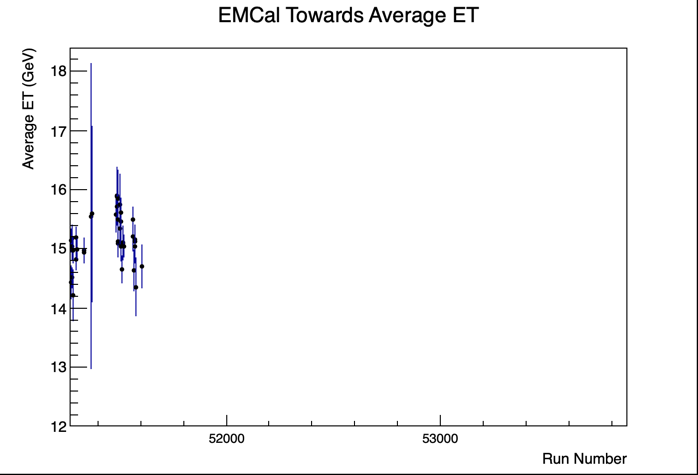
\includegraphics[width=\linewidth, trim=10 10 10 0, clip]{Figures/QA_Study/avg_et_emcal_towards_case6.png}
        \caption{EMCal: Towards region}
    \end{subfigure}
    \hfill
    \begin{subfigure}[t]{0.32\textwidth}
        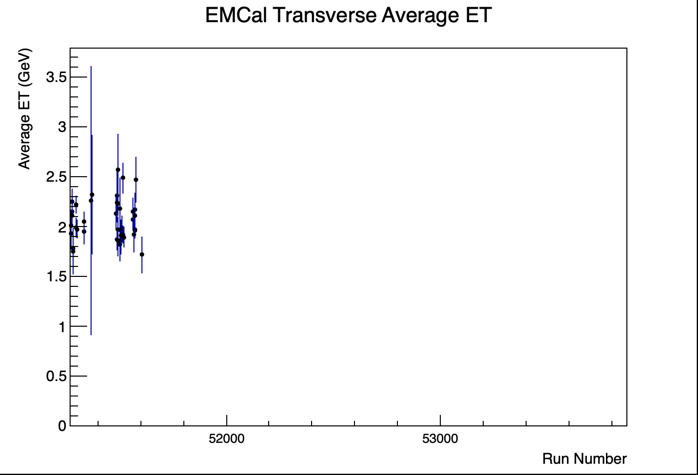
\includegraphics[width=\linewidth, trim=10 10 10 0, clip]{Figures/QA_Study/avg_et_emcal_transverse_case6.png}
        \caption{EMCal: Transverse region}
    \end{subfigure}
    \hfill
    \begin{subfigure}[t]{0.32\textwidth}
        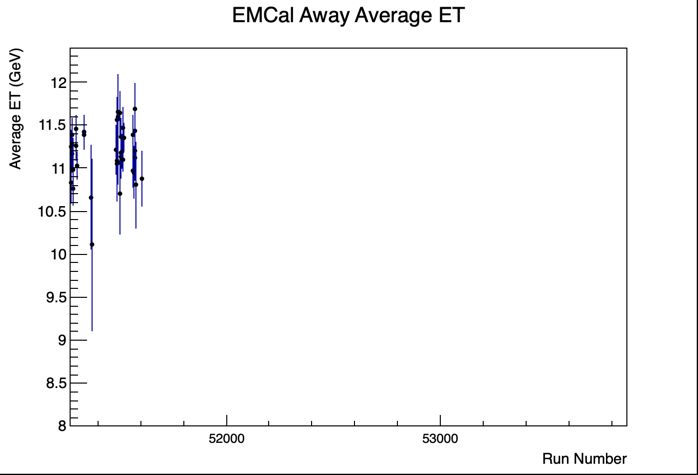
\includegraphics[width=\linewidth, trim=10 10 10 0, clip]{Figures/QA_Study/avg_et_emcal_away_case6.png}
        \caption{EMCal: Away region}
    \end{subfigure}
    \caption{Average transverse energy in EMCal for trigger 18 with \(p_T^{\text{lead}} > 15~\mathrm{GeV}/c\) .}
    \label{fig:avg_et_emcal_case6}
\end{figure}

\begin{figure}[H]
    \centering
    \begin{subfigure}[t]{0.32\textwidth}
        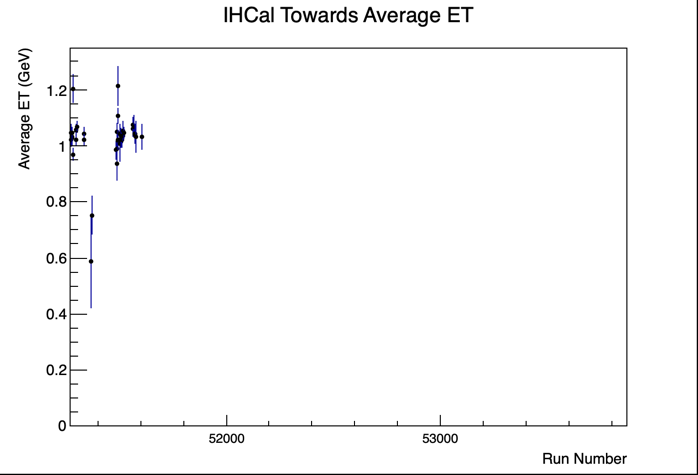
\includegraphics[width=\linewidth, trim=10 10 10 0, clip]{Figures/QA_Study/avg_et_ihcal_towards_case6.png}
        \caption{IHCal: Towards region}
    \end{subfigure}
    \hfill
    \begin{subfigure}[t]{0.32\textwidth}
        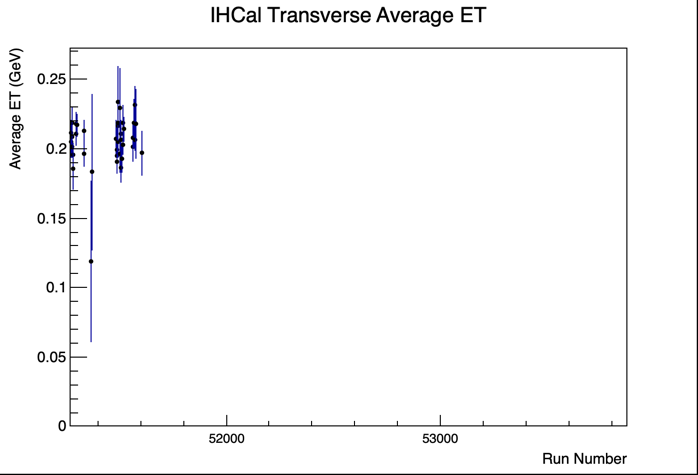
\includegraphics[width=\linewidth, trim=10 10 10 0, clip]{Figures/QA_Study/avg_et_ihcal_transverse_case6.png}
        \caption{IHCal: Transverse region}
    \end{subfigure}
    \hfill
    \begin{subfigure}[t]{0.32\textwidth}
        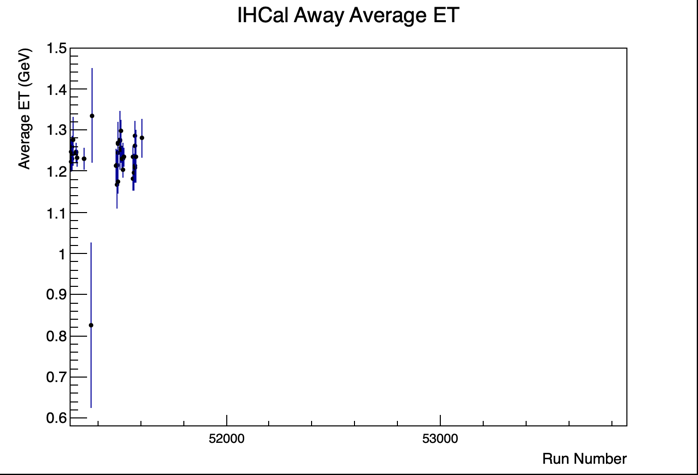
\includegraphics[width=\linewidth, trim=10 10 10 0, clip]{Figures/QA_Study/avg_et_ihcal_away_case6.png}
        \caption{IHCal: Away region}
    \end{subfigure}
    \caption{Average transverse energy in IHCal for trigger 18 with \(p_T^{\text{lead}} > 15~\mathrm{GeV}/c\) .}
    \label{fig:avg_et_ihcal_case6}
\end{figure}

\begin{figure}[H]
    \centering
    \begin{subfigure}[t]{0.32\textwidth}
        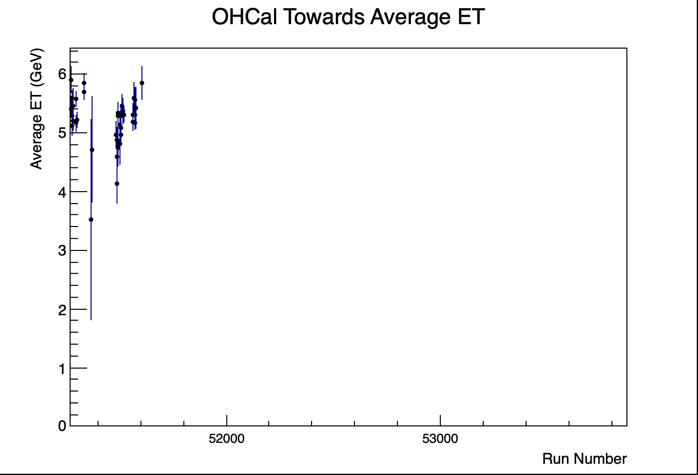
\includegraphics[width=\linewidth, trim=10 10 10 0, clip]{Figures/QA_Study/avg_et_ohcal_towards_case6.png}
        \caption{OHCal: Towards region}
    \end{subfigure}
    \hfill
    \begin{subfigure}[t]{0.32\textwidth}
        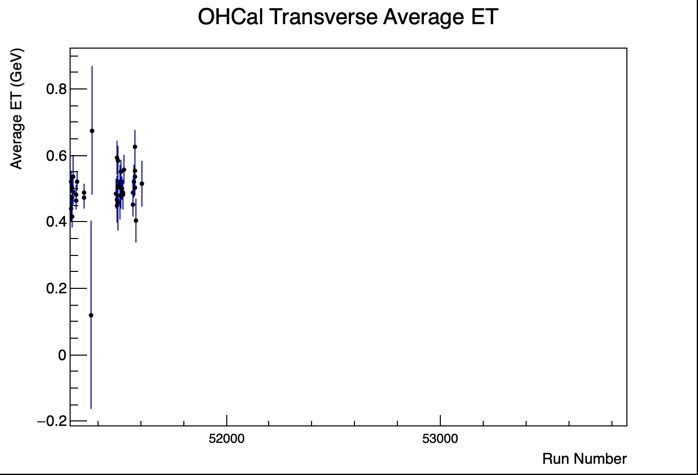
\includegraphics[width=\linewidth, trim=10 10 10 0, clip]{Figures/QA_Study/avg_et_ohcal_transverse_case6.png}
        \caption{OHCal: Transverse region}
    \end{subfigure}
    \hfill
    \begin{subfigure}[t]{0.32\textwidth}
        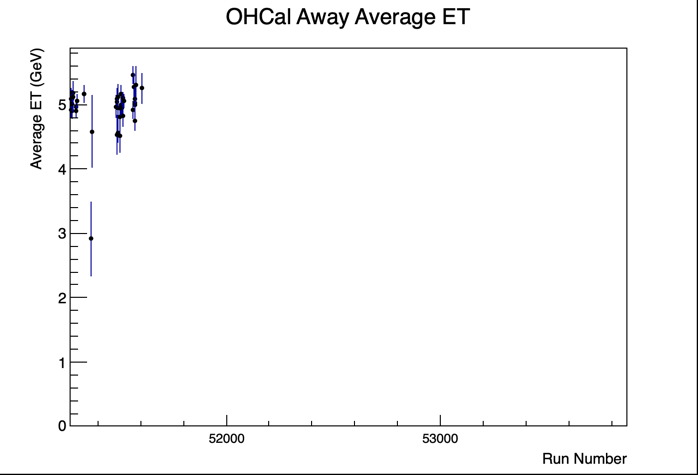
\includegraphics[width=\linewidth, trim=10 10 10 0, clip]{Figures/QA_Study/avg_et_ohcal_away_case6.png}
        \caption{OHCal: Away region}
    \end{subfigure}
    \caption{Average transverse energy in OHCal for trigger 18 with \(p_T^{\text{lead}} > 15~\mathrm{GeV}/c\) .}
    \label{fig:avg_et_ohcal_case6}
\end{figure}

For trigger 34, the average transverse energy distributions were analyzed under the selection \(p_T^{\text{lead}} > 15~\mathrm{GeV}/c\) and \(p_T^{\text{sublead}} > 0.3 \times p_T^{\text{lead}}\), using the same region-based decomposition of the detector: towards, transverse, and away. The results are consistent with previous observations.

In the EMCal, the average transverse energy is approximately \(15~\mathrm{GeV}\) in the towards region, \(2~\mathrm{GeV}\) in the transverse region, and \(11~\mathrm{GeV}\) in the away region. In the IHCal, the values are around \(1~\mathrm{GeV}\), \(0.2~\mathrm{GeV}\), and \(1.2~\mathrm{GeV}\), while the OHCal shows values near \(5.3~\mathrm{GeV}\), \(0.5~\mathrm{GeV}\), and \(5~\mathrm{GeV}\), respectively. These consistent measurements further validate the stability of the calorimeter performance and energy reconstruction under varying trigger conditions.

\begin{figure}[H]
    \centering
    \begin{subfigure}[t]{0.32\textwidth}
        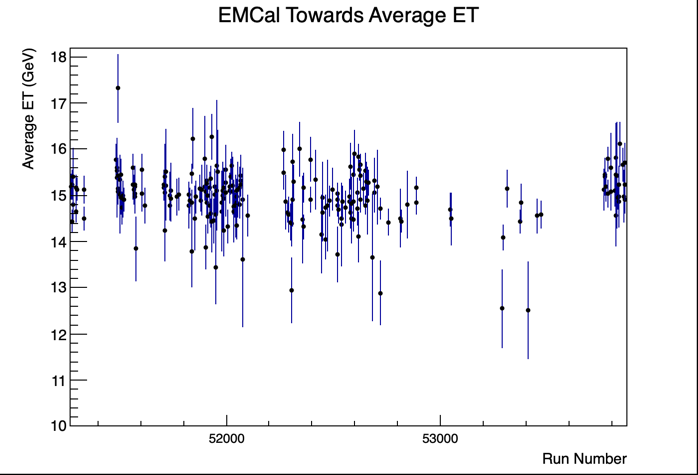
\includegraphics[width=\linewidth, trim=10 10 10 0, clip]{Figures/QA_Study/avg_et_emcal_towards_case7.png}
        \caption{EMCal: Towards region}
    \end{subfigure}
    \hfill
    \begin{subfigure}[t]{0.32\textwidth}
        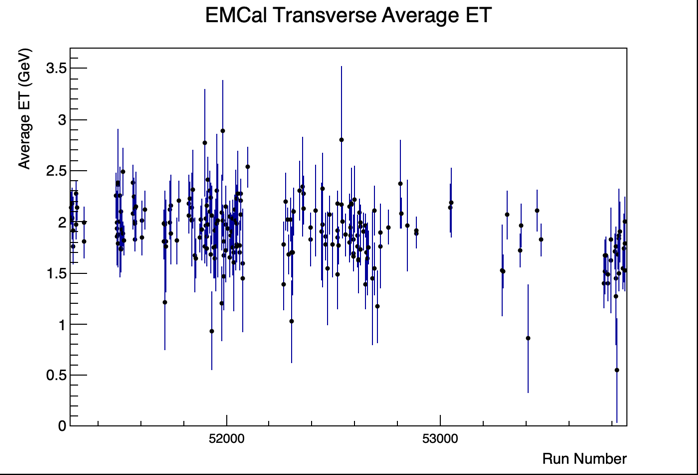
\includegraphics[width=\linewidth, trim=10 10 10 0, clip]{Figures/QA_Study/avg_et_emcal_transverse_case7.png}
        \caption{EMCal: Transverse region}
    \end{subfigure}
    \hfill
    \begin{subfigure}[t]{0.32\textwidth}
        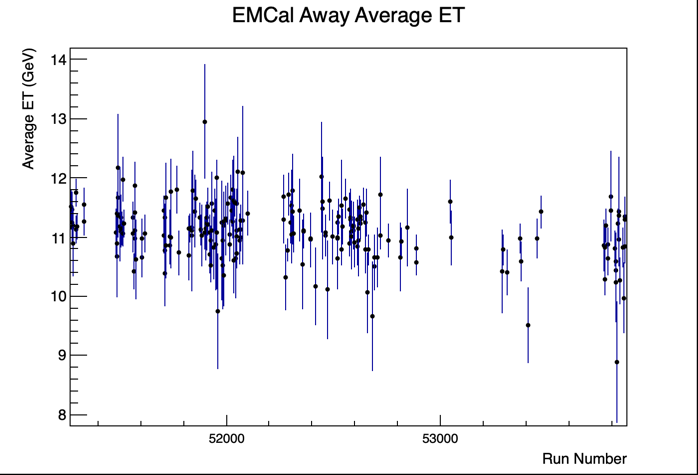
\includegraphics[width=\linewidth, trim=10 10 10 0, clip]{Figures/QA_Study/avg_et_emcal_away_case7.png}
        \caption{EMCal: Away region}
    \end{subfigure}
    \caption{Average transverse energy in EMCal for trigger 34 with \(p_T^{\text{lead}} > 15~\mathrm{GeV}/c\) .}
    \label{fig:avg_et_emcal_case7_t34}
\end{figure}

\begin{figure}[H]
    \centering
    \begin{subfigure}[t]{0.32\textwidth}
        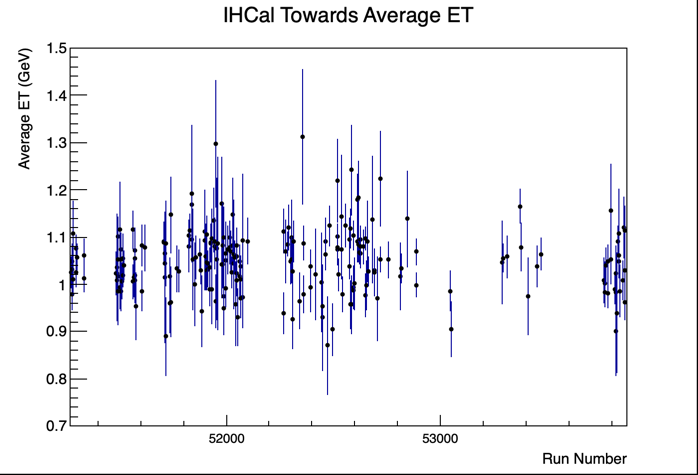
\includegraphics[width=\linewidth, trim=10 10 10 0, clip]{Figures/QA_Study/avg_et_ihcal_towards_case7.png}
        \caption{IHCal: Towards region}
    \end{subfigure}
    \hfill
    \begin{subfigure}[t]{0.32\textwidth}
        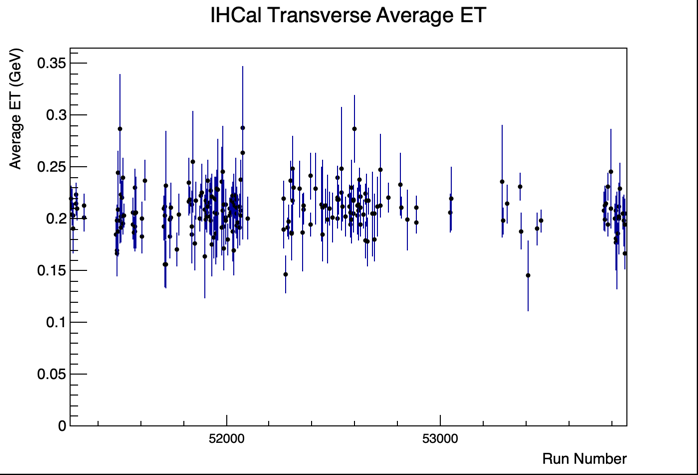
\includegraphics[width=\linewidth, trim=10 10 10 0, clip]{Figures/QA_Study/avg_et_ihcal_transverse_case7.png}
        \caption{IHCal: Transverse region}
    \end{subfigure}
    \hfill
    \begin{subfigure}[t]{0.32\textwidth}
        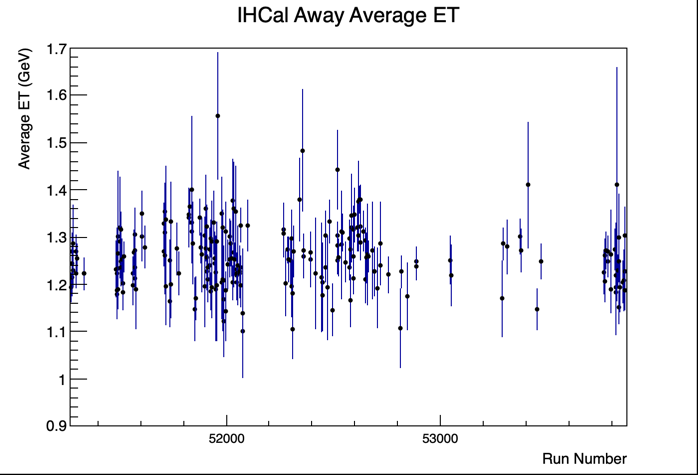
\includegraphics[width=\linewidth, trim=10 10 10 0, clip]{Figures/QA_Study/avg_et_ihcal_away_case7.png}
        \caption{IHCal: Away region}
    \end{subfigure}
    \caption{Average transverse energy in IHCal for trigger 34 with \(p_T^{\text{lead}} > 15~\mathrm{GeV}/c\) .}
    \label{fig:avg_et_ihcal_case7_t34}
\end{figure}

\begin{figure}[H]
    \centering
    \begin{subfigure}[t]{0.32\textwidth}
        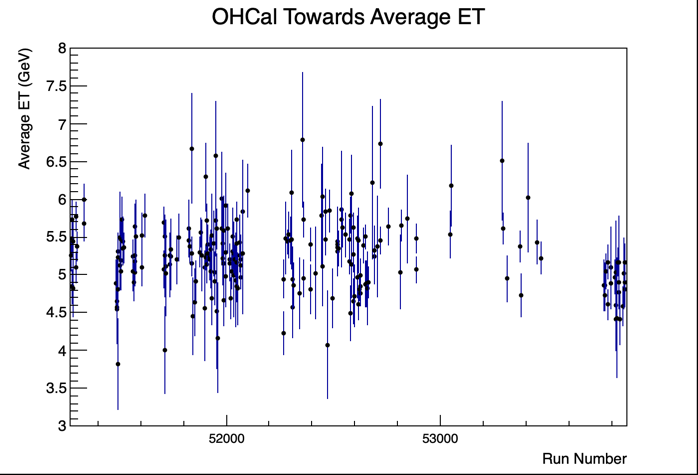
\includegraphics[width=\linewidth, trim=10 10 10 0, clip]{Figures/QA_Study/avg_et_ohcal_towards_case7.png}
        \caption{OHCal: Towards region}
    \end{subfigure}
    \hfill
    \begin{subfigure}[t]{0.32\textwidth}
        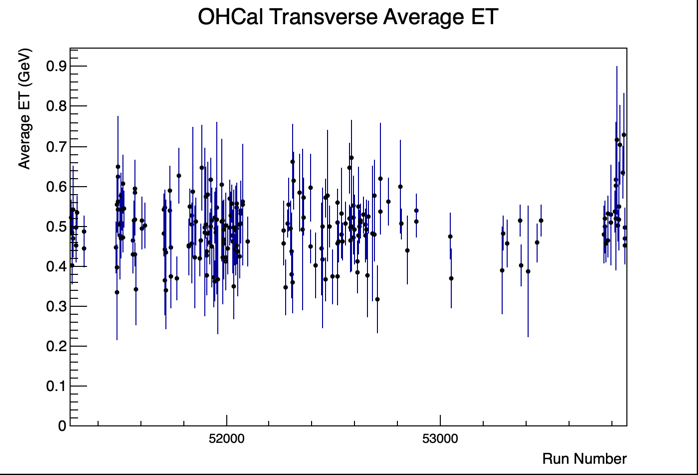
\includegraphics[width=\linewidth, trim=10 10 10 0, clip]{Figures/QA_Study/avg_et_ohcal_transverse_case7.png}
        \caption{OHCal: Transverse region}
    \end{subfigure}
    \hfill
    \begin{subfigure}[t]{0.32\textwidth}
        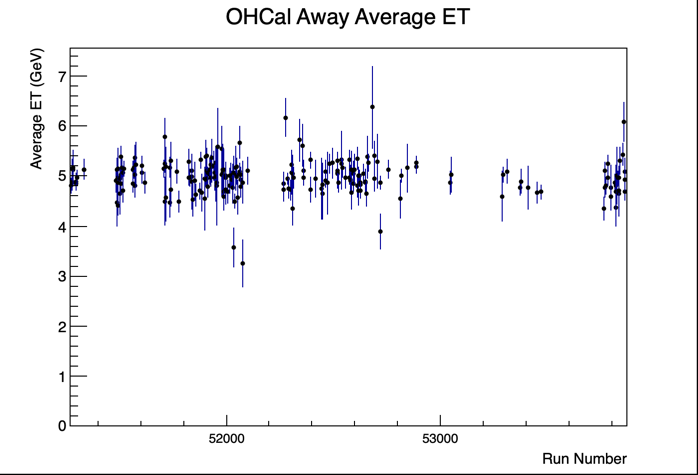
\includegraphics[width=\linewidth, trim=10 10 10 0, clip]{Figures/QA_Study/avg_et_ohcal_away_case7.png}
        \caption{OHCal: Away region}
    \end{subfigure}
    \caption{Average transverse energy in OHCal for trigger 34 with \(p_T^{\text{lead}} > 15~\mathrm{GeV}/c\) .}
    \label{fig:avg_et_ohcal_case7_t34}
\end{figure}

To further evaluate the energy deposition patterns using a different reconstruction approach, the average transverse energy per event was studied using EMCal clusters rather than towers. This analysis was conducted for triggers 16–23 and 32–35 under the jet selection criteria \(p_T^{\text{lead}} > 12~\mathrm{GeV}/c\) and \(p_T^{\text{sublead}} > 0.3 \times p_T^{\text{lead}}\).

The average transverse energy in the towards region is approximately \(18~\mathrm{GeV}\), showing a slight upward trend across run numbers. A similar pattern is observed in the transverse region, where the average is around \(9~\mathrm{GeV}\), and in the away region with an average close to \(15~\mathrm{GeV}\). These distributions are consistent with the expected energy flow in dijet events and support the stability of the EMCal cluster performance over time.
\begin{figure}[H]
    \centering
    \begin{subfigure}[t]{0.32\linewidth}
        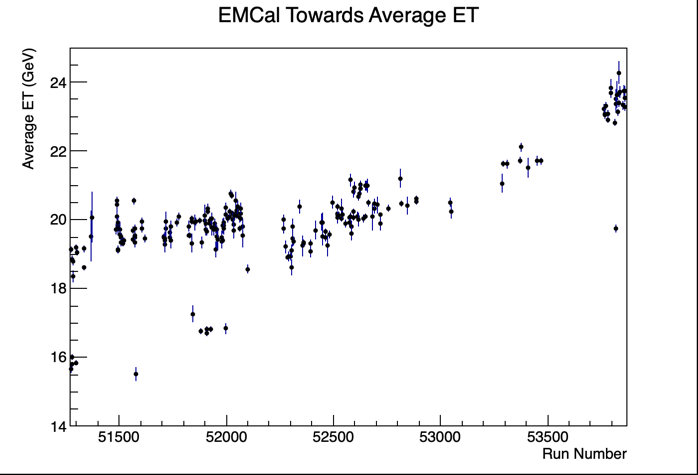
\includegraphics[width=\linewidth, trim=10 10 10 0, clip]{Figures/QA_Study/avg_et_cluster_towards_case1.png}
        \caption{Towards region}
        \label{fig:et_cluster_towards_case1}
    \end{subfigure}
    \hfill
    \begin{subfigure}[t]{0.32\linewidth}
        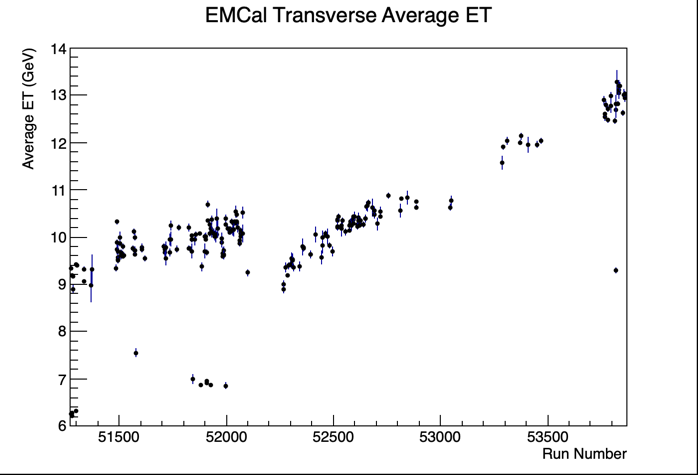
\includegraphics[width=\linewidth, trim=10 10 10 0, clip]{Figures/QA_Study/avg_et_cluster_transverse_case1.png}
        \caption{Transverse region}
        \label{fig:et_cluster_transverse_case1}
    \end{subfigure}
    \hfill
    \begin{subfigure}[t]{0.32\linewidth}
        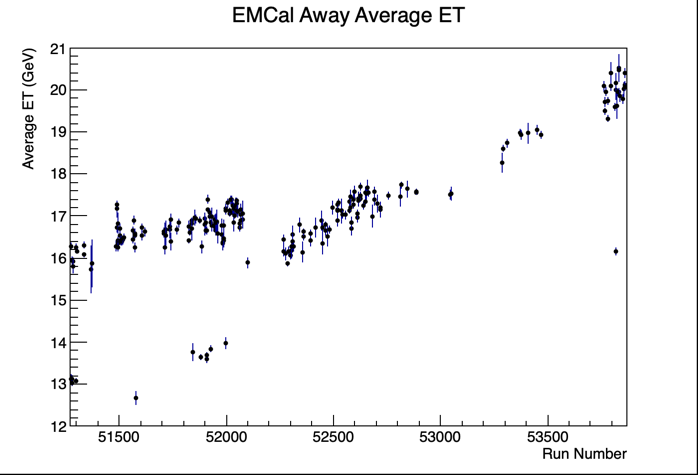
\includegraphics[width=\linewidth, trim=10 10 10 0, clip]{Figures/QA_Study/avg_et_cluster_away_case1.png}
        \caption{Away region}
        \label{fig:et_cluster_away_case1}
    \end{subfigure}
    \caption{Average transverse energy from EMCal clusters versus run number for triggers 16–23 and 32–35. Jet selection: \(p_T^{\text{lead}} > 12~\mathrm{GeV}/c\), \(p_T^{\text{sublead}} > 0.3 \times p_T^{\text{lead}}\).}
    \label{fig:avg_et_cluster_case1}
\end{figure}
A similar EMCal cluster analysis was performed for events selected with trigger 18, applying the same jet selection criteria of \( p_T^{\text{lead}} > 12~\mathrm{GeV}/c \) and \( p_T^{\text{sublead}} > 0.3 \times p_T^{\text{lead}} \). The average transverse energy per event was calculated in the towards, transverse, and away regions as a function of run number. The results are consistent with those observed for other triggers. In the EMCal, the towards region shows an average transverse energy of approximately 18~GeV with a mild increasing trend over time. The transverse region displays an average around 9~GeV, while the away region exhibits an average near 15~GeV. These findings reinforce the reliability of the EMCal cluster-based measurements across the full data-taking period for this trigger.
\begin{figure}[H]
    \centering
    \begin{subfigure}[t]{0.32\linewidth}
        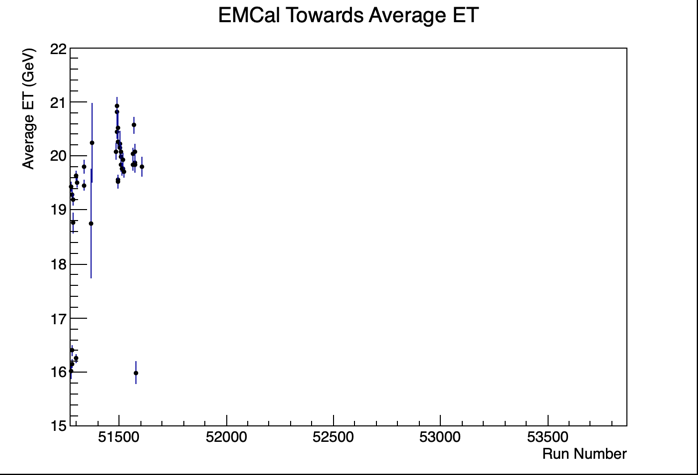
\includegraphics[width=\linewidth, trim=10 10 10 0, clip]{Figures/QA_Study/avg_et_cluster_towards_case2.png}
        \caption{Towards region}
        \label{fig:et_cluster_towards_case2}
    \end{subfigure}
    \hfill
    \begin{subfigure}[t]{0.32\linewidth}
        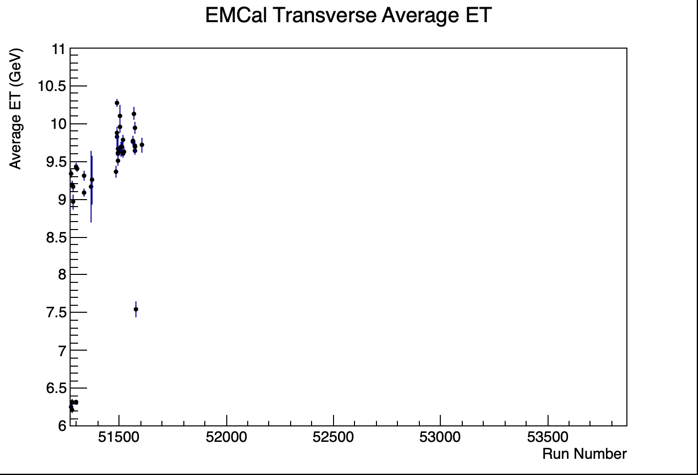
\includegraphics[width=\linewidth, trim=10 10 10 0, clip]{Figures/QA_Study/avg_et_cluster_transverse_case2.png}
        \caption{Transverse region}
        \label{fig:et_cluster_transverse_case2}
    \end{subfigure}
    \hfill
    \begin{subfigure}[t]{0.32\linewidth}
        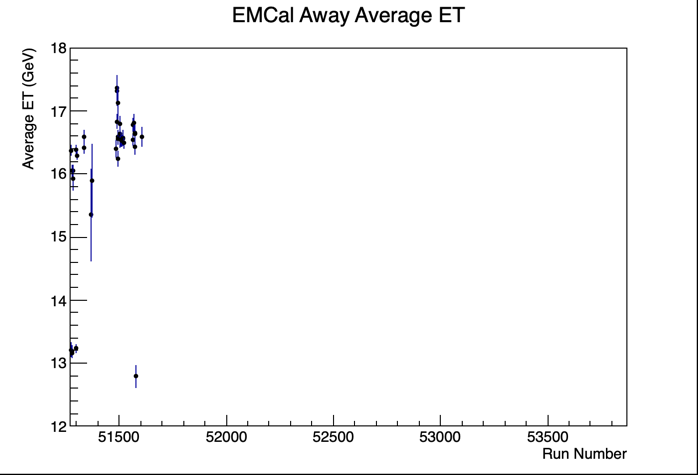
\includegraphics[width=\linewidth, trim=10 10 10 0, clip]{Figures/QA_Study/avg_et_cluster_away_case2.png}
        \caption{Away region}
        \label{fig:et_cluster_away_case2}
    \end{subfigure}
    \caption{Average transverse energy from EMCal clusters versus run number for trigger 18 (case 2). Jet selection: \(p_T^{\text{lead}} > 12~\mathrm{GeV}/c\), \(p_T^{\text{sublead}} > 0.3 \times p_T^{\text{lead}}\).}
    \label{fig:avg_et_cluster_case2}
\end{figure}
The EMCal cluster-based transverse energy analysis was also extended to events triggered with trigger 34, under the same jet selection of \( p_T^{\text{lead}} > 12~\mathrm{GeV}/c \) and \( p_T^{\text{sublead}} > 0.3 \times p_T^{\text{lead}} \). The average transverse energy per event is presented for the towards, transverse, and away regions across the full range of run numbers. Consistent with previous results, the towards region exhibits an average transverse energy around 18~GeV, with a slight upward trend over time. In the transverse region, the average is approximately 9~GeV, while the away region shows an average of about 15~GeV. These observations confirm the stable and consistent behavior of EMCal cluster energy measurements across multiple triggers.
\begin{figure}[H]
    \centering
    \begin{subfigure}[t]{0.32\linewidth}
        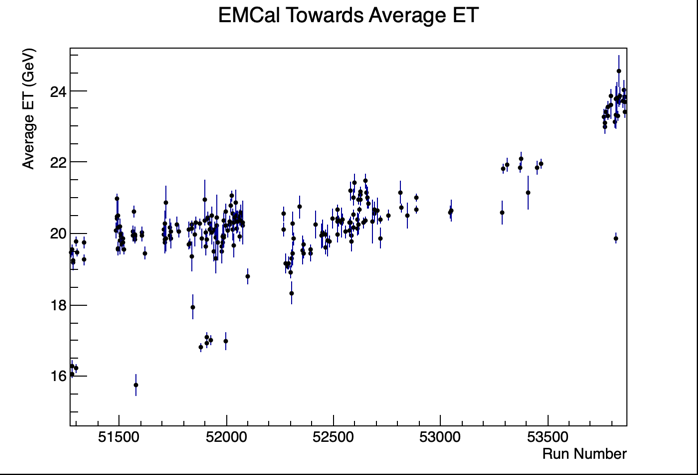
\includegraphics[width=\linewidth, trim=10 10 10 0, clip]{Figures/QA_Study/avg_et_cluster_towards_case3.png}
        \caption{Towards region}
        \label{fig:et_cluster_towards_case3}
    \end{subfigure}
    \hfill
    \begin{subfigure}[t]{0.32\linewidth}
        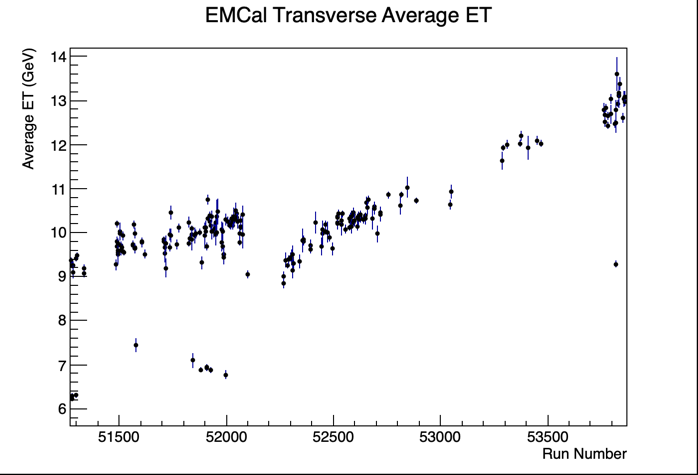
\includegraphics[width=\linewidth, trim=10 10 10 0, clip]{Figures/QA_Study/avg_et_cluster_transverse_case3.png}
        \caption{Transverse region}
        \label{fig:et_cluster_transverse_case3}
    \end{subfigure}
    \hfill
    \begin{subfigure}[t]{0.32\linewidth}
        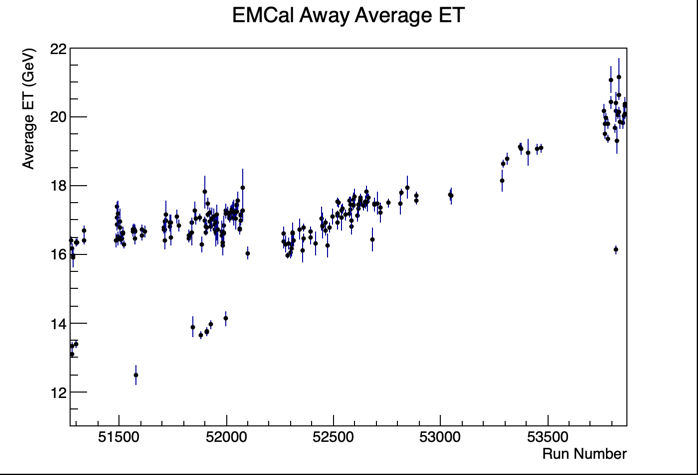
\includegraphics[width=\linewidth, trim=10 10 10 0, clip]{Figures/QA_Study/avg_et_cluster_away_case3.png}
        \caption{Away region}
        \label{fig:et_cluster_away_case3}
    \end{subfigure}
    \caption{Average transverse energy from EMCal clusters versus run number for trigger 34 (case 3). Jet selection: \(p_T^{\text{lead}} > 12~\mathrm{GeV}/c\), \(p_T^{\text{sublead}} > 0.3 \times p_T^{\text{lead}}\).}
    \label{fig:avg_et_cluster_case3}
\end{figure}
The EMCal cluster-based average transverse energy was also examined for the combined trigger selection of 16–23 and 32–35, applying a stricter jet transverse momentum requirement: \( p_T^{\text{lead}} > 15~\mathrm{GeV}/c \) and \( p_T^{\text{sublead}} > 0.3 \times p_T^{\text{lead}} \). The transverse energy distributions as a function of run number are analyzed in the towards, transverse, and away regions. The results show a slightly increasing trend in energy over time. Specifically, the average transverse energy in the towards region is around 21~GeV, approximately 9~GeV in the transverse region, and around 17~GeV in the away region. These observations reflect consistent detector performance and energy reconstruction under higher jet energy thresholds.
\begin{figure}[H]
    \centering
    \begin{subfigure}[t]{0.32\linewidth}
        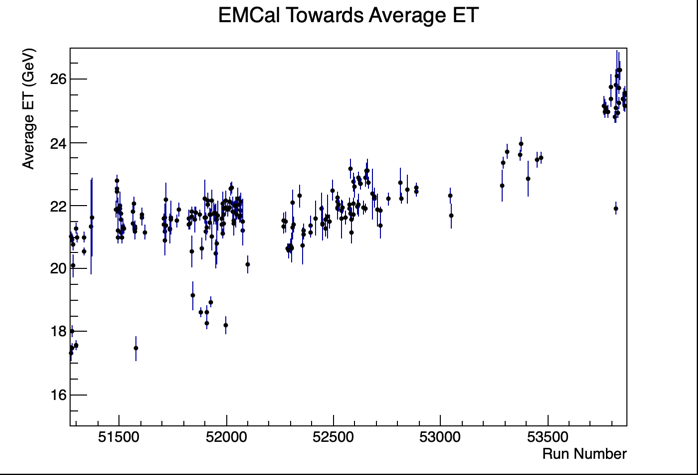
\includegraphics[width=\linewidth, trim=10 10 10 0, clip]{Figures/QA_Study/avg_et_cluster_towards_case4.png}
        \caption{Towards region}
        \label{fig:et_cluster_towards_case4}
    \end{subfigure}
    \hfill
    \begin{subfigure}[t]{0.32\linewidth}
        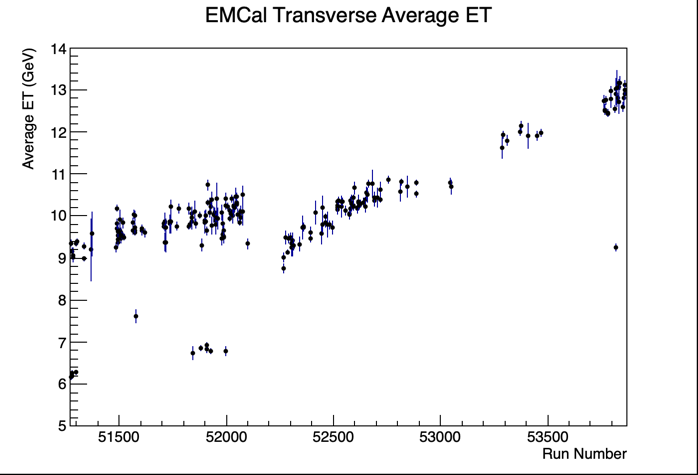
\includegraphics[width=\linewidth, trim=10 10 10 0, clip]{Figures/QA_Study/avg_et_cluster_transverse_case4.png}
        \caption{Transverse region}
        \label{fig:et_cluster_transverse_case4}
    \end{subfigure}
    \hfill
    \begin{subfigure}[t]{0.32\linewidth}
        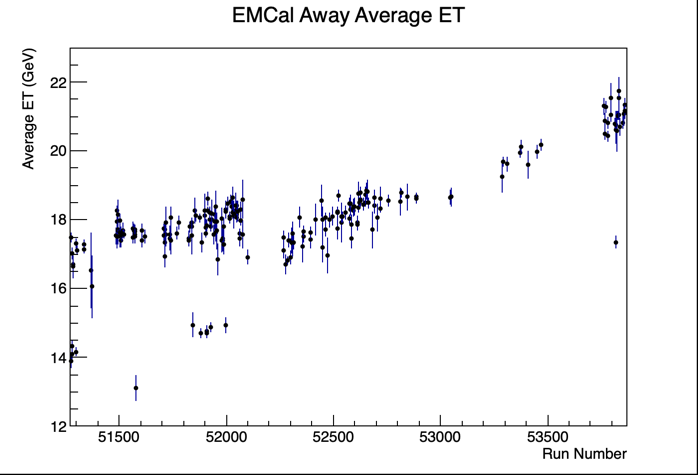
\includegraphics[width=\linewidth, trim=10 10 10 0, clip]{Figures/QA_Study/avg_et_cluster_away_case4.png}
        \caption{Away region}
        \label{fig:et_cluster_away_case4}
    \end{subfigure}
    \caption{Average transverse energy from EMCal clusters versus run number for triggers 16–23 and 32–35 (case 4). Jet selection: \(p_T^{\text{lead}} > 15~\mathrm{GeV}/c\), \(p_T^{\text{sublead}} > 0.3 \times p_T^{\text{lead}}\).}
    \label{fig:avg_et_cluster_case4}
\end{figure}
The average transverse energy measured using EMCal clusters was further evaluated for events selected with trigger 18, applying the condition \( p_T^{\text{lead}} > 15~\mathrm{GeV}/c \) and \( p_T^{\text{sublead}} > 0.3 \times p_T^{\text{lead}} \). The analysis was carried out across the standard azimuthal regions: towards, transverse, and away. The results indicate a stable and slightly increasing trend in average transverse energy across run numbers. Specifically, the average energy is approximately 21~GeV in the towards region, 9~GeV in the transverse region, and 17~GeV in the away region. These values are consistent with earlier findings, demonstrating the reliable performance of the EMCal cluster-based energy reconstruction under higher jet momentum thresholds.
\begin{figure}[H]
    \centering
    \begin{subfigure}[t]{0.32\linewidth}
        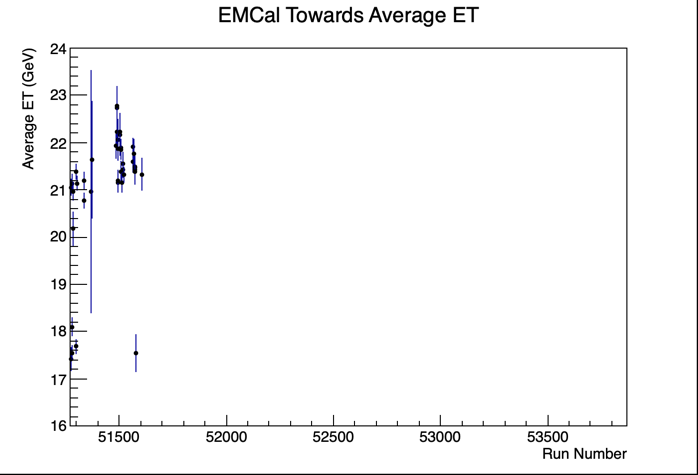
\includegraphics[width=\linewidth, trim=10 10 10 0, clip]{Figures/QA_Study/avg_et_cluster_towards_case5.png}
        \caption{Towards region}
        \label{fig:et_cluster_towards_case5}
    \end{subfigure}
    \hfill
    \begin{subfigure}[t]{0.32\linewidth}
        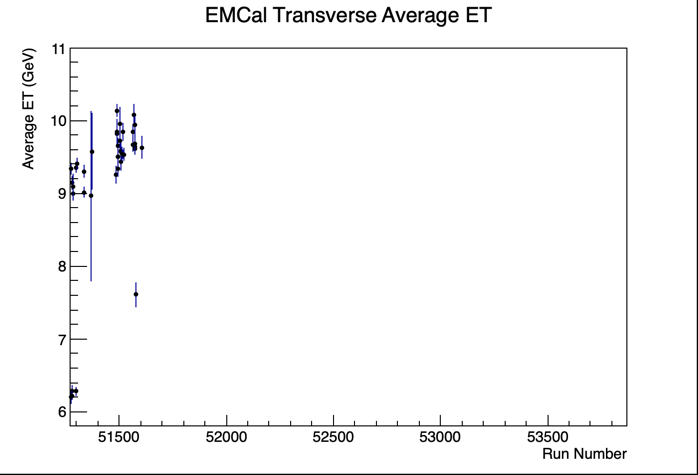
\includegraphics[width=\linewidth, trim=10 10 10 0, clip]{Figures/QA_Study/avg_et_cluster_transverse_case5.png}
        \caption{Transverse region}
        \label{fig:et_cluster_transverse_case5}
    \end{subfigure}
    \hfill
    \begin{subfigure}[t]{0.32\linewidth}
        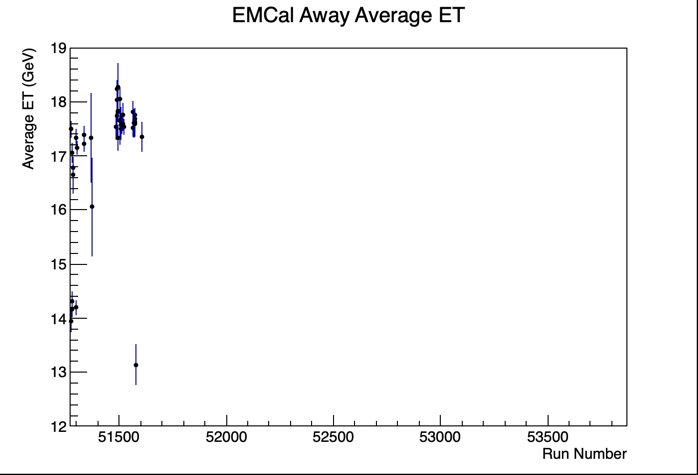
\includegraphics[width=\linewidth, trim=10 10 10 0, clip]{Figures/QA_Study/avg_et_cluster_away_case5.png}
        \caption{Away region}
        \label{fig:et_cluster_away_case5}
    \end{subfigure}
    \caption{Average transverse energy from EMCal clusters versus run number for trigger 18 (case 5). Jet selection: \(p_T^{\text{lead}} > 15~\mathrm{GeV}/c\), \(p_T^{\text{sublead}} > 0.3 \times p_T^{\text{lead}}\).}
    \label{fig:avg_et_cluster_case5}
\end{figure}
For events selected with trigger 34, the average transverse energy measured from EMCal clusters was studied under the selection criteria of \( p_T^{\text{lead}} > 15~\mathrm{GeV}/c \) and \( p_T^{\text{sublead}} > 0.3 \times p_T^{\text{lead}} \). The results exhibit consistent behavior with previous triggers and selections. In the towards region, the average transverse energy is approximately 21~GeV, while in the transverse region it is around 9~GeV, and about 17~GeV in the away region. Furthermore, the values show a slight increasing trend over time. These observations reinforce the stability of the EMCal cluster-based energy measurements across varying trigger and jet selection conditions.
\begin{figure}[H]
    \centering
    \begin{subfigure}[t]{0.32\linewidth}
        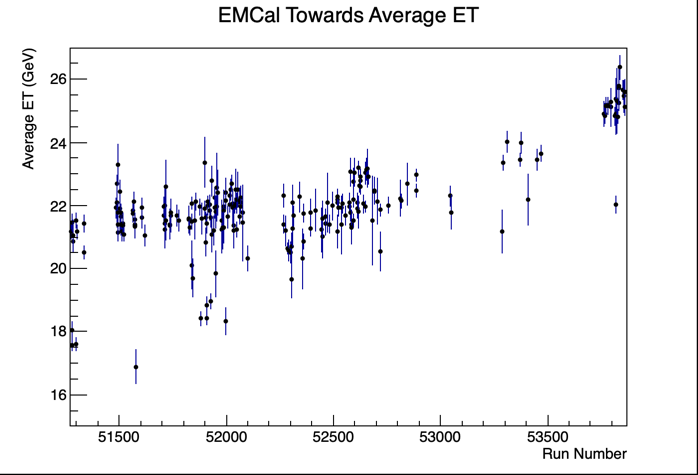
\includegraphics[width=\linewidth, trim=10 10 10 0, clip]{Figures/QA_Study/avg_et_cluster_towards_case6.png}
        \caption{Towards region}
        \label{fig:et_cluster_towards_case6}
    \end{subfigure}
    \hfill
    \begin{subfigure}[t]{0.32\linewidth}
        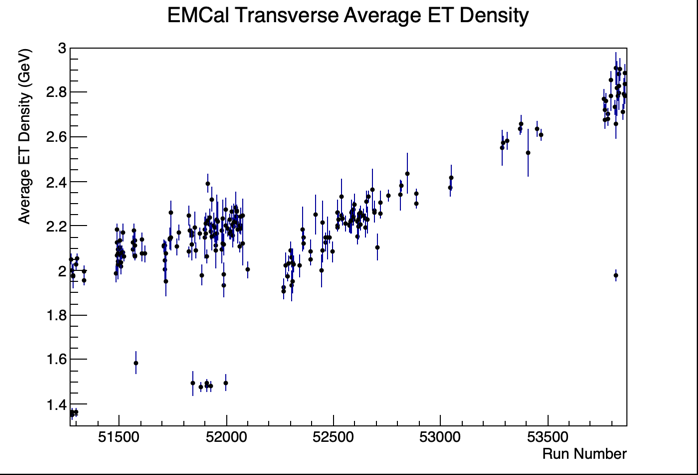
\includegraphics[width=\linewidth, trim=10 10 10 0, clip]{Figures/QA_Study/avg_et_cluster_transverse_case6.png}
        \caption{Transverse region}
        \label{fig:et_cluster_transverse_case6}
    \end{subfigure}
    \hfill
    \begin{subfigure}[t]{0.32\linewidth}
        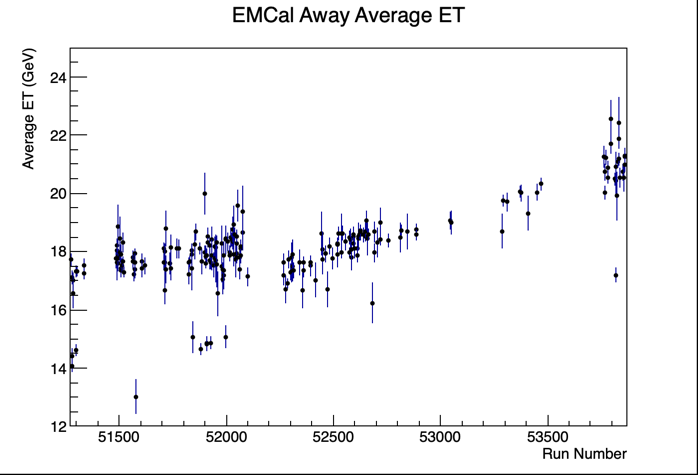
\includegraphics[width=\linewidth, trim=10 10 10 0, clip]{Figures/QA_Study/avg_et_cluster_away_case6.png}
        \caption{Away region}
        \label{fig:et_cluster_away_case6}
    \end{subfigure}
    \caption{Average transverse energy from EMCal clusters versus run number for trigger 34 (case 6). Jet selection: \(p_T^{\text{lead}} > 15~\mathrm{GeV}/c\), \(p_T^{\text{sublead}} > 0.3 \times p_T^{\text{lead}}\).}
    \label{fig:avg_et_cluster_case6}
\end{figure}
The average transverse energy per event based on topoclusters was evaluated as a function of run number for events selected with triggers 16–23 and 32–35. The jet selection requires \( p_T^{\text{lead}} > 12~\mathrm{GeV}/c \) and \( p_T^{\text{sublead}} > 0.3 \times p_T^{\text{lead}} \). In the towards region, the average transverse energy is approximately 15.5~GeV, while in the transverse region it is around 1.4~GeV. In the away region, the average transverse energy is about 12~GeV. These values are stable across the run range, indicating good performance of the topocluster-based reconstruction under the applied selection conditions.
\begin{figure}[H]
    \centering
    \begin{subfigure}[t]{0.32\linewidth}
        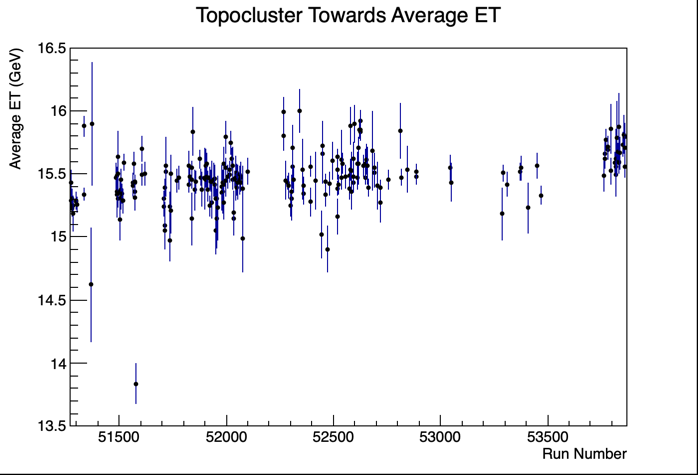
\includegraphics[width=\linewidth, trim=10 10 10 0, clip]{Figures/QA_Study/avg_et_topo_towards_case1.png}
        \caption{Towards region}
        \label{fig:et_topo_towards_case1}
    \end{subfigure}
    \hfill
    \begin{subfigure}[t]{0.32\linewidth}
        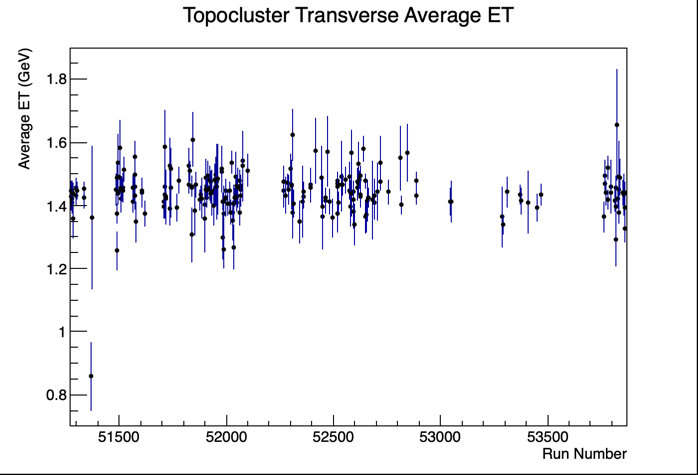
\includegraphics[width=\linewidth, trim=10 10 10 0, clip]{Figures/QA_Study/avg_et_topo_transverse_case1.png}
        \caption{Transverse region}
        \label{fig:et_topo_transverse_case1}
    \end{subfigure}
    \hfill
    \begin{subfigure}[t]{0.32\linewidth}
        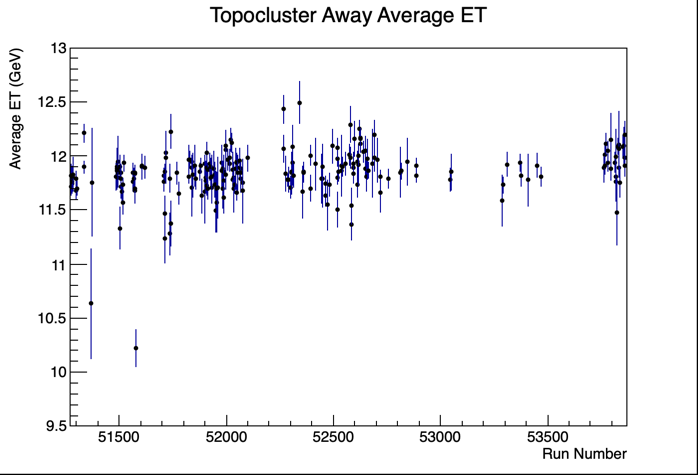
\includegraphics[width=\linewidth, trim=10 10 10 0, clip]{Figures/QA_Study/avg_et_topo_away_case1.png}
        \caption{Away region}
        \label{fig:et_topo_away_case1}
    \end{subfigure}
    \caption{Average transverse energy from topoclusters versus run number for triggers 16–23 and 32–35. Jet selection: \(p_T^{\text{lead}} > 12~\mathrm{GeV}/c\), \(p_T^{\text{sublead}} > 0.3 \times p_T^{\text{lead}}\).}
    \label{fig:avg_et_topo_case1}
\end{figure}
The performance of topocluster-based energy reconstruction was also evaluated for events triggered by trigger 18. The selection requires \( p_T^{\text{lead}} > 12~\mathrm{GeV}/c \) and \( p_T^{\text{sublead}} > 0.3 \times p_T^{\text{lead}} \). The average transverse energy per event is consistent with earlier observations: around 15.5~GeV in the towards region, approximately 1.4~GeV in the transverse region, and about 12~GeV in the away region. These results confirm the stability of the EMCal topocluster response under the specified selection conditions.
\begin{figure}[H]
    \centering
    \begin{subfigure}[t]{0.32\linewidth}
        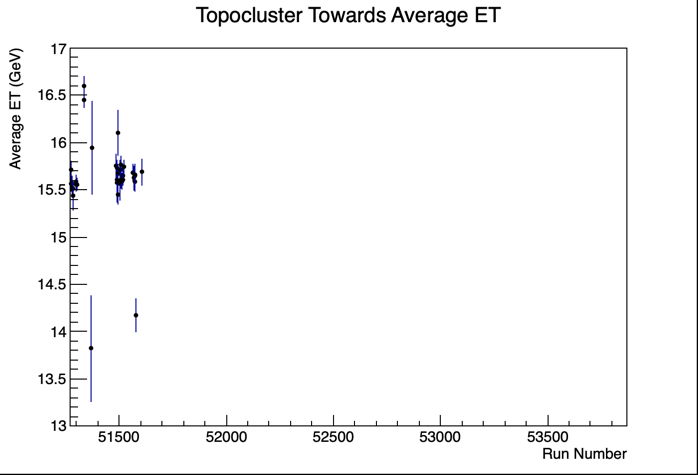
\includegraphics[width=\linewidth, trim=10 10 10 0, clip]{Figures/QA_Study/avg_et_topo_towards_case2.png}
        \caption{Towards region}
        \label{fig:et_topo_towards_case2}
    \end{subfigure}
    \hfill
    \begin{subfigure}[t]{0.32\linewidth}
        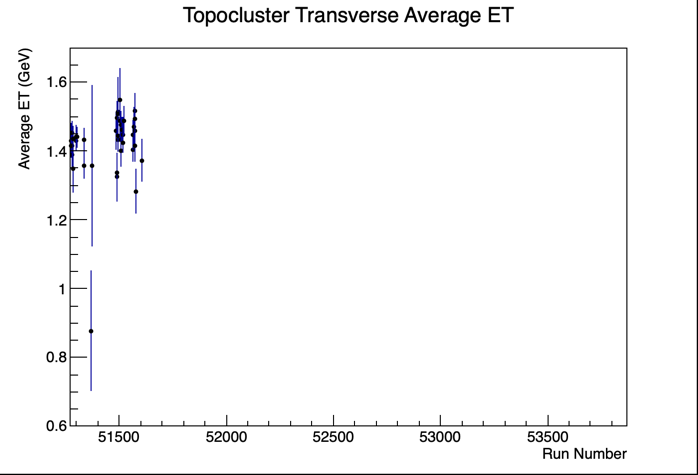
\includegraphics[width=\linewidth, trim=10 10 10 0, clip]{Figures/QA_Study/avg_et_topo_transverse_case2.png}
        \caption{Transverse region}
        \label{fig:et_topo_transverse_case2}
    \end{subfigure}
    \hfill
    \begin{subfigure}[t]{0.32\linewidth}
        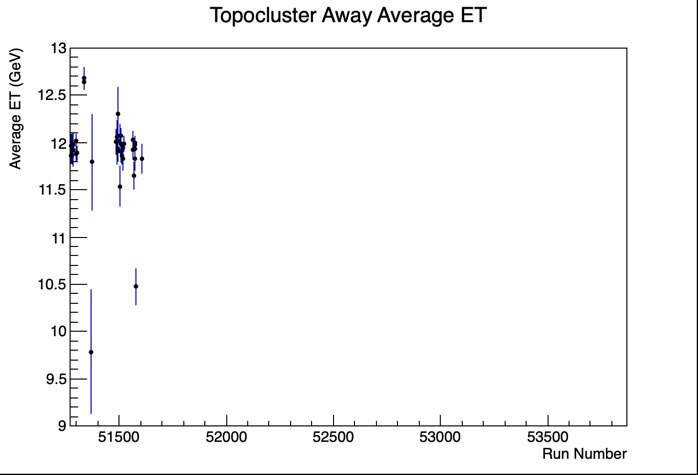
\includegraphics[width=\linewidth, trim=10 10 10 0, clip]{Figures/QA_Study/avg_et_topo_away_case2.png}
        \caption{Away region}
        \label{fig:et_topo_away_case2}
    \end{subfigure}
    \caption{Average transverse energy from topoclusters versus run number for trigger 18. Jet selection: \(p_T^{\text{lead}} > 12~\mathrm{GeV}/c\), \(p_T^{\text{sublead}} > 0.3 \times p_T^{\text{lead}}\).}
    \label{fig:avg_et_topo_case2}
\end{figure}
For events triggered by trigger 34, the average transverse energy measured from topoclusters shows similar stability and behavior as previous cases. With the jet selection criteria \( p_T^{\text{lead}} > 12~\mathrm{GeV}/c \) and \( p_T^{\text{sublead}} > 0.3 \times p_T^{\text{lead}} \), the average transverse energy is approximately 15.5~GeV in the towards region, 1.4~GeV in the transverse region, and about 12~GeV in the away region. This consistency underscores the reliability of topocluster reconstruction across different trigger conditions.
\begin{figure}[H]
    \centering
    \begin{subfigure}[t]{0.32\linewidth}
        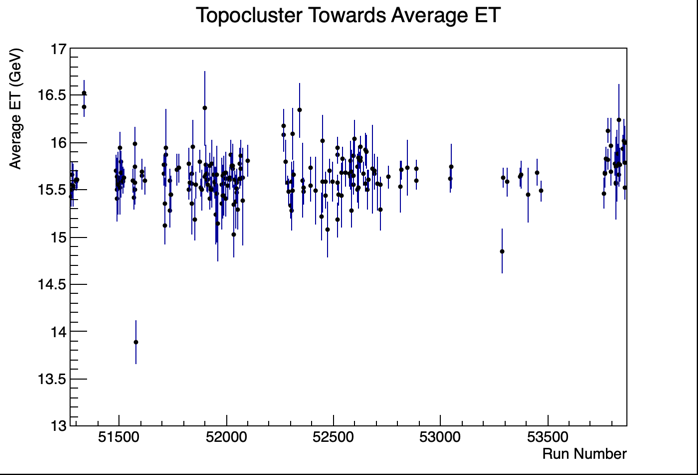
\includegraphics[width=\linewidth, trim=10 10 10 0, clip]{Figures/QA_Study/avg_et_topo_towards_case3.png}
        \caption{Towards region}
        \label{fig:et_topo_towards_case3}
    \end{subfigure}
    \hfill
    \begin{subfigure}[t]{0.32\linewidth}
        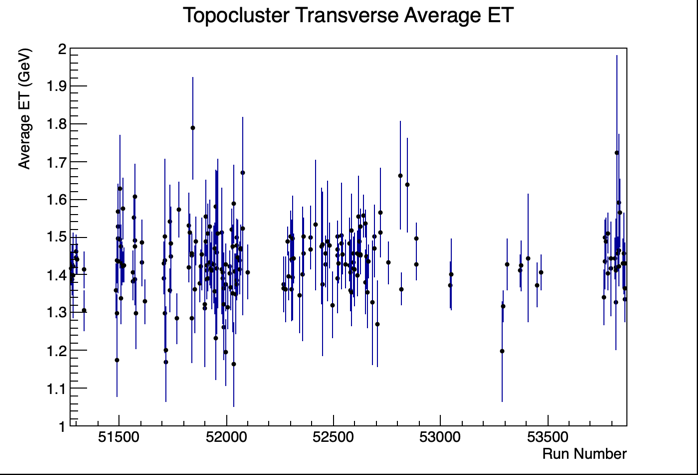
\includegraphics[width=\linewidth, trim=10 10 10 0, clip]{Figures/QA_Study/avg_et_topo_transverse_case3.png}
        \caption{Transverse region}
        \label{fig:et_topo_transverse_case3}
    \end{subfigure}
    \hfill
    \begin{subfigure}[t]{0.32\linewidth}
        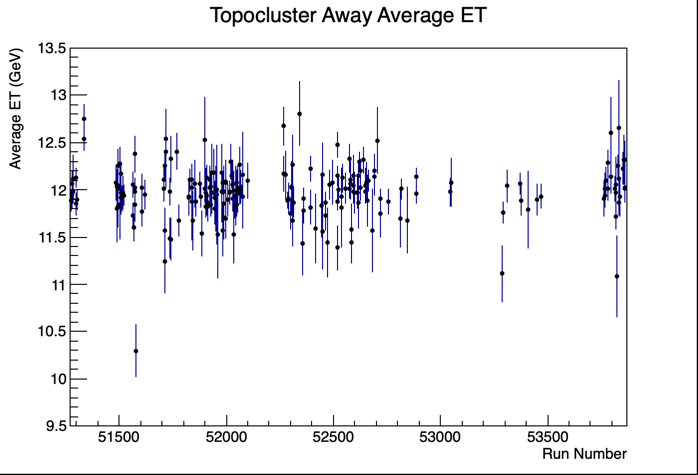
\includegraphics[width=\linewidth, trim=10 10 10 0, clip]{Figures/QA_Study/avg_et_topo_away_case3.png}
        \caption{Away region}
        \label{fig:et_topo_away_case3}
    \end{subfigure}
    \caption{Average transverse energy from topoclusters versus run number for trigger 34. Jet selection: \(p_T^{\text{lead}} > 12~\mathrm{GeV}/c\), \(p_T^{\text{sublead}} > 0.3 \times p_T^{\text{lead}}\).}
    \label{fig:avg_et_topo_case3}
\end{figure}
For the combined trigger range 16–23 and 32–35, with the increased jet selection threshold of \( p_T^{\text{lead}} > 15~\mathrm{GeV}/c \) and \( p_T^{\text{sublead}} > 0.3 \times p_T^{\text{lead}} \), the average transverse energy measured from topoclusters remains consistent across runs. Specifically, the average \( E_T \) is around 18~GeV in the towards region, approximately 1.4~GeV in the transverse region, and about 14~GeV in the away region. These values reflect the expected increase in energy deposition associated with the higher leading jet momentum and confirm the stability of the calorimetric response over the analyzed dataset.
\begin{figure}[H]
    \centering
    \begin{subfigure}[t]{0.32\linewidth}
        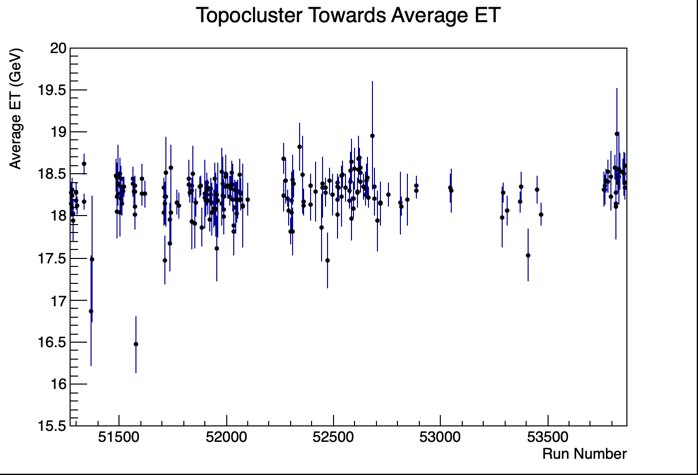
\includegraphics[width=\linewidth, trim=10 10 10 0, clip]{Figures/QA_Study/avg_et_topo_towards_case4.png}
        \caption{Towards region}
        \label{fig:et_topo_towards_case4}
    \end{subfigure}
    \hfill
    \begin{subfigure}[t]{0.32\linewidth}
        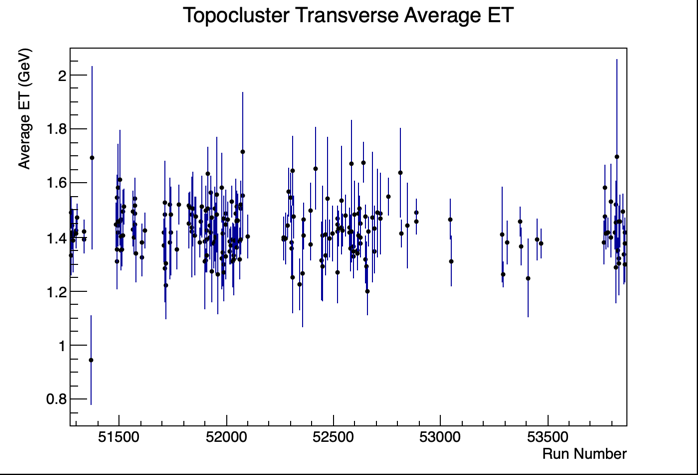
\includegraphics[width=\linewidth, trim=10 10 10 0, clip]{Figures/QA_Study/avg_et_topo_transverse_case4.png}
        \caption{Transverse region}
        \label{fig:et_topo_transverse_case4}
    \end{subfigure}
    \hfill
    \begin{subfigure}[t]{0.32\linewidth}
        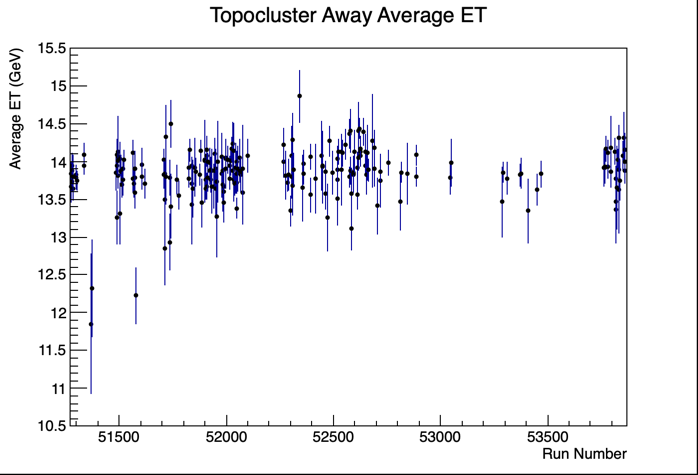
\includegraphics[width=\linewidth, trim=10 10 10 0, clip]{Figures/QA_Study/avg_et_topo_away_case4.png}
        \caption{Away region}
        \label{fig:et_topo_away_case4}
    \end{subfigure}
    \caption{Average transverse energy from topoclusters versus run number for triggers 16–23 and 32–35. Jet selection: \(p_T^{\text{lead}} > 15~\mathrm{GeV}/c\), \(p_T^{\text{sublead}} > 0.3 \times p_T^{\text{lead}}\).}
    \label{fig:avg_et_topo_case4}
\end{figure}
For events selected with trigger 18 and the higher jet selection threshold of \( p_T^{\text{lead}} > 15~\mathrm{GeV}/c \) and \( p_T^{\text{sublead}} > 0.3 \times p_T^{\text{lead}} \), the average transverse energy measured from topoclusters is consistent with previous results. Specifically, the average \( E_T \) is around 18~GeV in the towards region, approximately 1.4~GeV in the transverse region, and about 14~GeV in the away region. These stable values across runs reflect the expected behavior from increased jet activity and demonstrate the reliability of the topocluster reconstruction in different angular regions.
\begin{figure}[H]
    \centering
    \begin{subfigure}[t]{0.32\linewidth}
        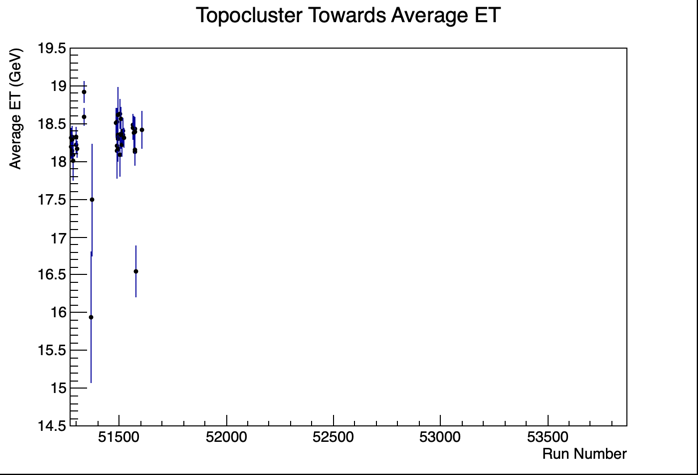
\includegraphics[width=\linewidth, trim=10 10 10 0, clip]{Figures/QA_Study/avg_et_topo_towards_case5.png}
        \caption{Towards region}
        \label{fig:et_topo_towards_case5}
    \end{subfigure}
    \hfill
    \begin{subfigure}[t]{0.32\linewidth}
        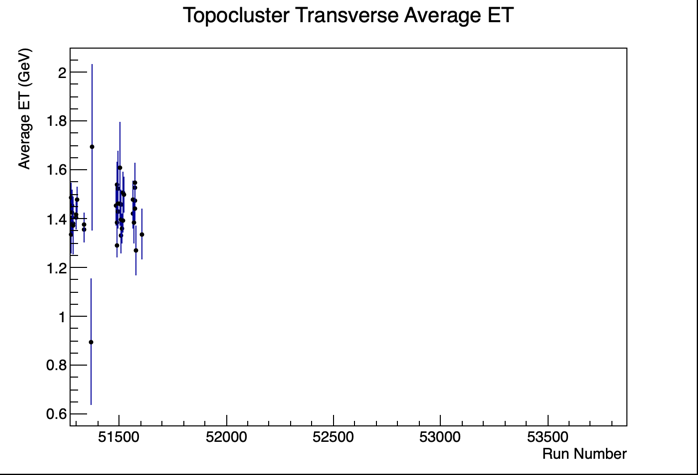
\includegraphics[width=\linewidth, trim=10 10 10 0, clip]{Figures/QA_Study/avg_et_topo_transverse_case5.png}
        \caption{Transverse region}
        \label{fig:et_topo_transverse_case5}
    \end{subfigure}
    \hfill
    \begin{subfigure}[t]{0.32\linewidth}
        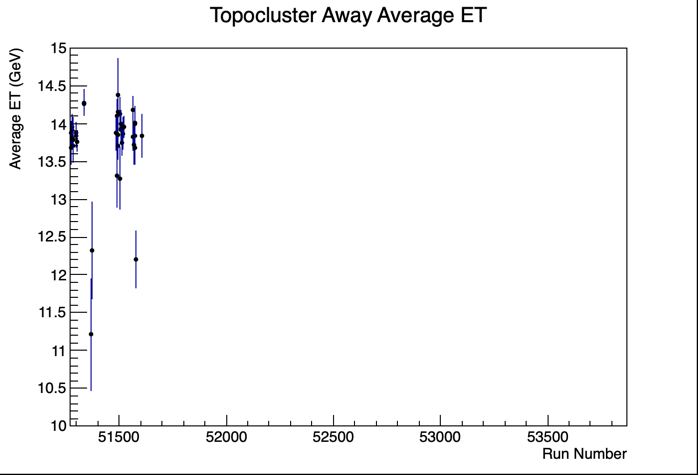
\includegraphics[width=\linewidth, trim=10 10 10 0, clip]{Figures/QA_Study/avg_et_topo_away_case5.png}
        \caption{Away region}
        \label{fig:et_topo_away_case5}
    \end{subfigure}
    \caption{Average transverse energy from topoclusters versus run number for trigger 18. Jet selection: \(p_T^{\text{lead}} > 15~\mathrm{GeV}/c\), \(p_T^{\text{sublead}} > 0.3 \times p_T^{\text{lead}}\).}
    \label{fig:avg_et_topo_case5}
\end{figure}
For trigger 34, using the selection of \( p_T^{\text{lead}} > 15~\mathrm{GeV}/c \) and \( p_T^{\text{sublead}} > 0.3 \times p_T^{\text{lead}} \), the average transverse energy from topoclusters exhibits similar behavior to previously observed patterns. The average \( E_T \) in the towards region is approximately 18~GeV, while the transverse region yields around 1.4~GeV, and the away region shows an average of about 14~GeV. These values confirm the consistency and robustness of topocluster-based energy reconstruction under varying jet topology and trigger conditions.
\begin{figure}[H]
    \centering
    \begin{subfigure}[t]{0.32\linewidth}
        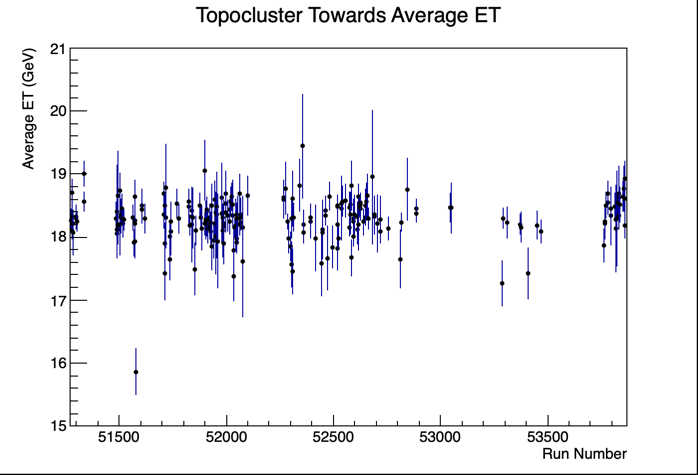
\includegraphics[width=\linewidth, trim=10 10 10 0, clip]{Figures/QA_Study/avg_et_topo_towards_case6.png}
        \caption{Towards region}
        \label{fig:et_topo_towards_case6}
    \end{subfigure}
    \hfill
    \begin{subfigure}[t]{0.32\linewidth}
        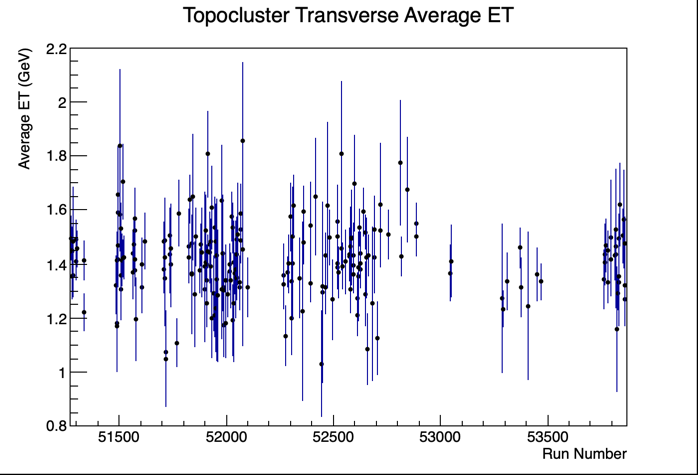
\includegraphics[width=\linewidth, trim=10 10 10 0, clip]{Figures/QA_Study/avg_et_topo_transverse_case6.png}
        \caption{Transverse region}
        \label{fig:et_topo_transverse_case6}
    \end{subfigure}
    \hfill
    \begin{subfigure}[t]{0.32\linewidth}
        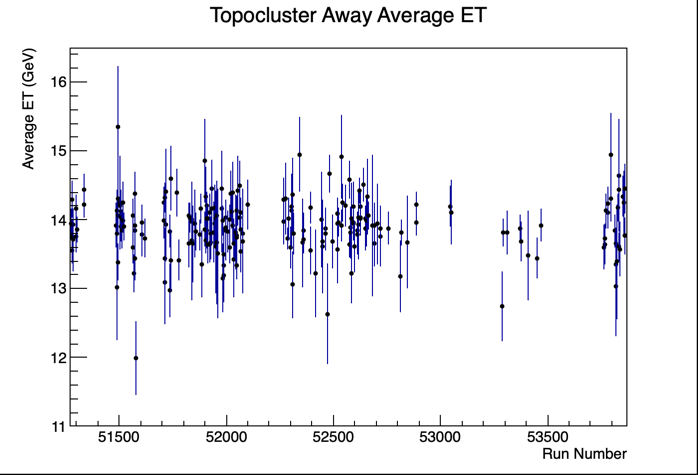
\includegraphics[width=\linewidth, trim=10 10 10 0, clip]{Figures/QA_Study/avg_et_topo_away_case6.png}
        \caption{Away region}
        \label{fig:et_topo_away_case6}
    \end{subfigure}
    \caption{Average transverse energy from topoclusters versus run number for trigger 34. Jet selection: \(p_T^{\text{lead}} > 15~\mathrm{GeV}/c\), \(p_T^{\text{sublead}} > 0.3 \times p_T^{\text{lead}}\).}
    \label{fig:avg_et_topo_case6}
\end{figure}


\subsubsection{Defining jet event geometry}
To study the underlying event in regions outside of the jet cone, the following event geometry is defined by the $\phi$ direction of the leading $\pT$ jet. The calorimeter acceptance is split up into three azimuthal regions with respect to the $\phi$ direction of the leading jet. The towards region with $\|\Delta\phi\| < 60 \degree$ from the leading jet, two transverse regions with $ 60 \degree < \|\Delta \phi\| < 120 \degree$ and an away region with $\|\Delta\phi\| > 120 \degree$. The towards, transverse and away regions are shown in Fig. \ref{fig:event_geometry}. 
\begin{figure}[H]
    \centering
    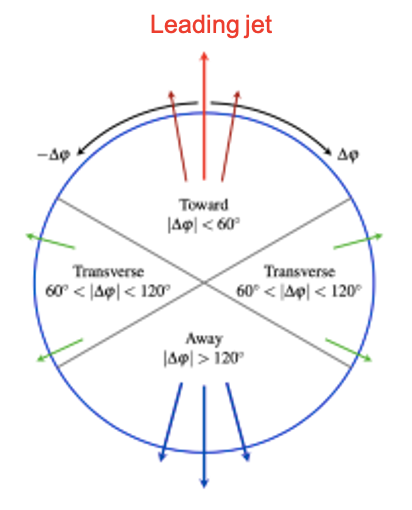
\includegraphics[width=0.3\linewidth]{Figures/event_geometry.png}
    \caption{Towards, transverse and away region definitions of jet event with respect to the leading jet azimuthal direction.}
    \label{fig:event_geometry}
\end{figure}

\subsection{Topocluster reconstruction}
Topoclusters are created using all three layers of the calorimeters. The default topoclustering parameters are as follows: 
\begin{verbatim}
  RawClusterBuilderTopo* ClusterBuilder = new 
            RawClusterBuilderTopo("HcalRawClusterBuilderTopo");
  ClusterBuilder->Verbosity(verbosity);
  ClusterBuilder->set_nodename("TOPOCLUSTER_ALLCALO");
  ClusterBuilder->set_enable_HCal(true);
  ClusterBuilder->set_enable_EMCal(true);
  ClusterBuilder->set_noise(IHCal_noise, OHCal_noise, EMCal_noise);
  ClusterBuilder->set_significance(4.0, 2.0, 0.0);
  ClusterBuilder->allow_corner_neighbor(true);
  ClusterBuilder->set_do_split(true);
  ClusterBuilder->set_minE_local_max(1.0, 2.0, 0.5);
  ClusterBuilder->set_R_shower(0.025);
  ClusterBuilder->set_use_only_good_towers(true);
  ClusterBuilder->set_absE(true);
  se->registerSubsystem(ClusterBuilder);  
\end{verbatim}

\subsubsection{Setting topocluster noise thresholds}
Topocluster noise thresholds are optimized for the state of the calorimeter noise during the Run 2024 p+p 1.5mrad running by first finding the tower-by-tower pedestal RMS for each calorimeter layer from pedestal data (Run 54256) seen in Figure~\ref{fig:pedestal_RMS}, scaling the overall pedestal spectra from this run to match the pedestal region of beam runs from 1.5mrad p+p data, and then testing truth particle to topocluster matching for two, three and four times the average tower-by-tower pedestal RMS of the calorimeter layer using the Run 22 minbias simulation sample with realistic pedestal noise embedded. The resulting noise parameters used for the analysis are: 68.4 MeV for the EMCal, 5.3 MeV for the IHCal and 35.1 MeV for the OHCal. 

\begin{figure}
    \centering
    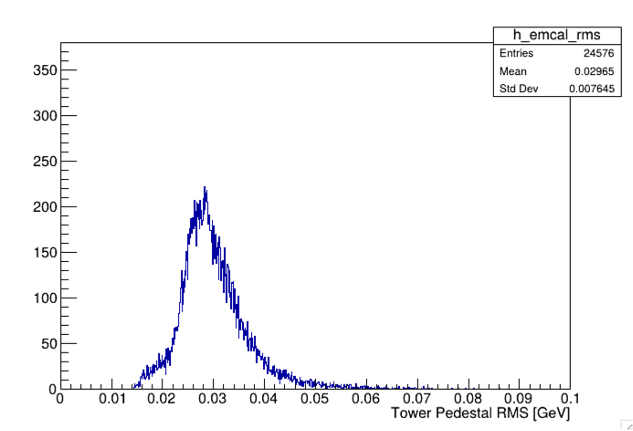
\includegraphics[width=0.32\linewidth]{Figures/topocluster_noise/emcal_pedestal_rms.png}
    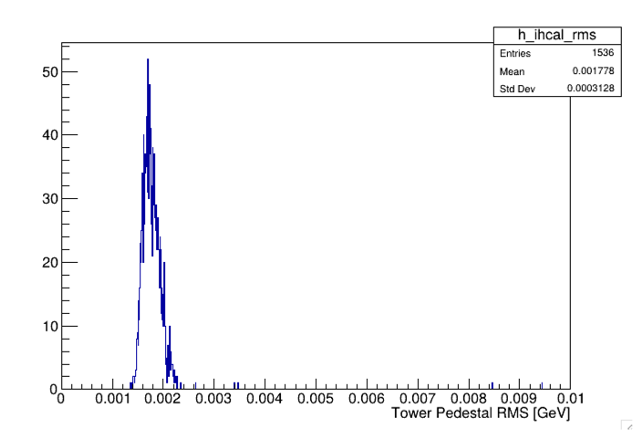
\includegraphics[width=0.32\linewidth]{Figures/topocluster_noise/ihcal_pedestal_rms.png}
    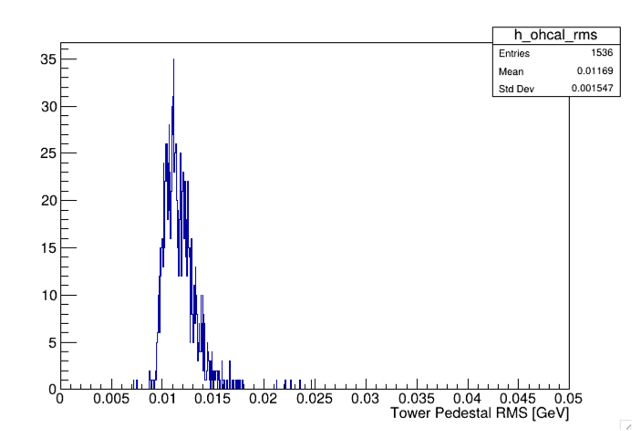
\includegraphics[width=0.32\linewidth]{Figures/topocluster_noise/ohcal_pedestal_rms.png}
    \caption{Tower-by-tower pedestal RMS for EMCal (left), IHCal (middle) and OHCal (right) found from pedestal run 54256. Mean RMS is extracted, scaled to match pedestal in beam data and used for testing noise thresholds in topocluster seeding.}
    \label{fig:pedestal_RMS}
\end{figure}

\textcolor{blue}{Add in information about and histograms of topocluster noise studies done by Ghosoun for analysis here.}
\subsection{Resolution of Topoclusters}

The resolution of topoclusters is studied separately for electromagnetic (EM) and hadronic particles, using two distance thresholds: $\Delta R < 0.1$ and $\Delta R < 0.2$. To ensure the quality of the matched truth–reconstructed pairs, specific selection criteria are applied. An isolation condition is enforced, requiring the truth particle to have no other nearby truth particles with transverse momentum $p_T > 0.2$\,GeV within a cone of $\Delta R < 0.6$. Additionally, only particles satisfying $|z| < 30$\,cm are considered. 

The analysis is performed for three noise suppression thresholds: $2\sigma$, $3\sigma$, and $4\sigma$. These thresholds are used to evaluate how noise impacts the resolution performance of topoclusters.

For EM particles, the properties of the closest matched topocluster are examined. Only clusters with energy $E > 1$\,GeV are included. The resolution is quantified using the $E/P$ ratio, where $E$ is the energy of the matched cluster and $P$ is the momentum of the corresponding truth particle. Figure~\ref{fig:ep_resolution} shows the $E/P$ distributions for different noise thresholds at $\Delta R < 0.1$.

\begin{figure}[H]
  \centering
  \begin{subfigure}[b]{0.31\textwidth}
    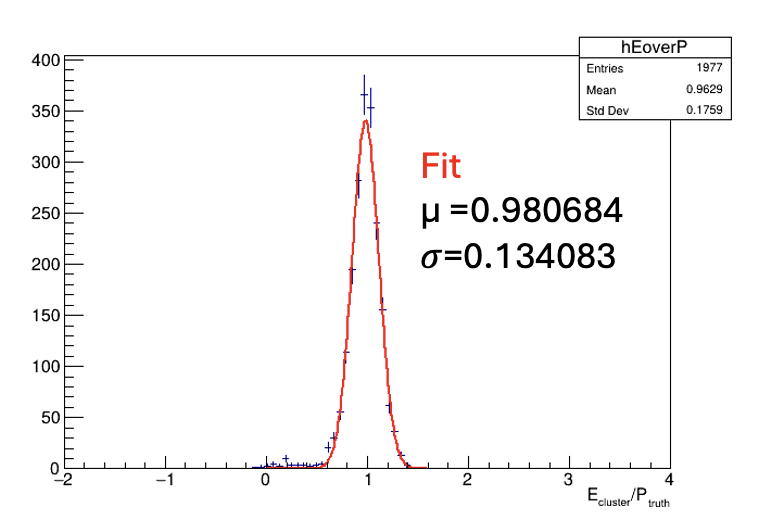
\includegraphics[width=\textwidth]{Figures/topocluster_noise/Resolution_topocluster/ep_2sigma.png}
    \caption{$2\sigma$}
  \end{subfigure}
  \hfill
  \begin{subfigure}[b]{0.32\textwidth}
    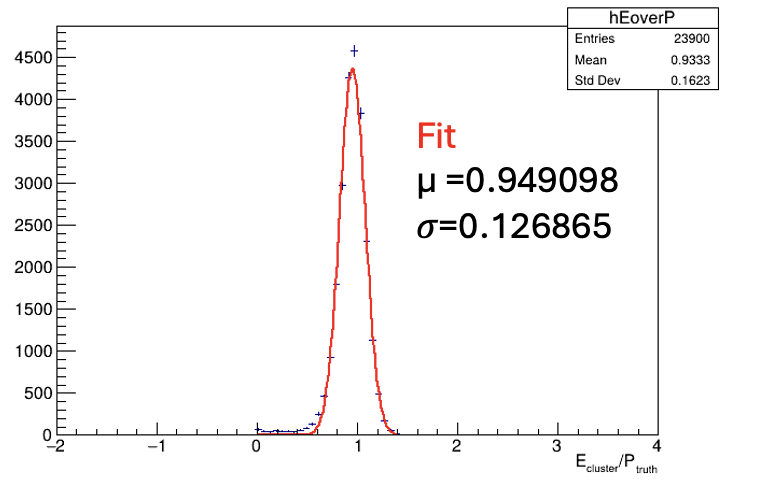
\includegraphics[width=\textwidth]{Figures/topocluster_noise/Resolution_topocluster/ep_3sigma.png}
    \caption{$3\sigma$}
  \end{subfigure}
  \hfill
  \begin{subfigure}[b]{0.31\textwidth}
    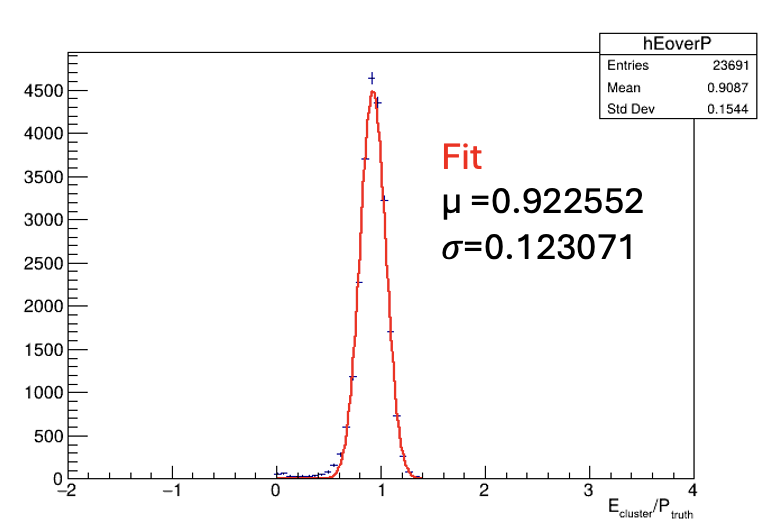
\includegraphics[width=\textwidth]{Figures/topocluster_noise/Resolution_topocluster/ep_4sigma.png}
    \caption{$4\sigma$}
  \end{subfigure}
  \caption{$E/P$ distributions for electromagnetic particles at $\Delta R < 0.1$ for different noise thresholds.}
  \label{fig:ep_resolution}
\end{figure}
The extracted resolutions from these distributions are 13.7\%, 13.4\%, and 13.3\% for the $2\sigma$, $3\sigma$, and $4\sigma$ thresholds, respectively. These values are consistent with results obtained from test beam measurements. The $E/P$ distributions for different noise thresholds at $\Delta R < 0.2$ are also studied, as shown in Fig.~\ref{fig:ep_resolution_dr02}.
\begin{figure}[h]
  \centering
  \begin{subfigure}[b]{0.32\textwidth}
    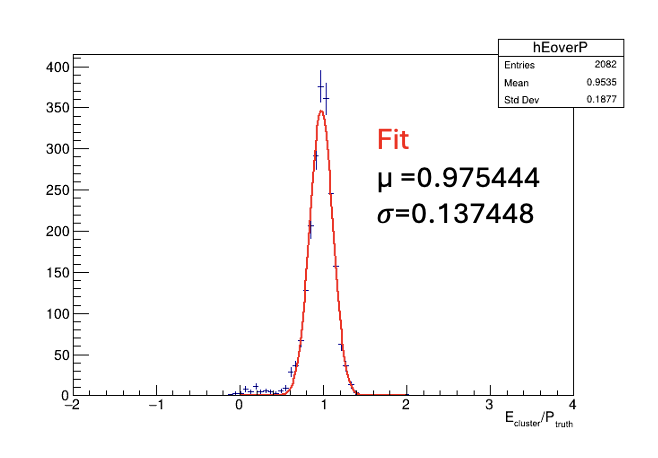
\includegraphics[width=\textwidth]{Figures/topocluster_noise/Resolution_topocluster/ep_2sigma_dr02.png}
    \caption{$2\sigma$}
  \end{subfigure}
  \hfill
  \begin{subfigure}[b]{0.32\textwidth}
    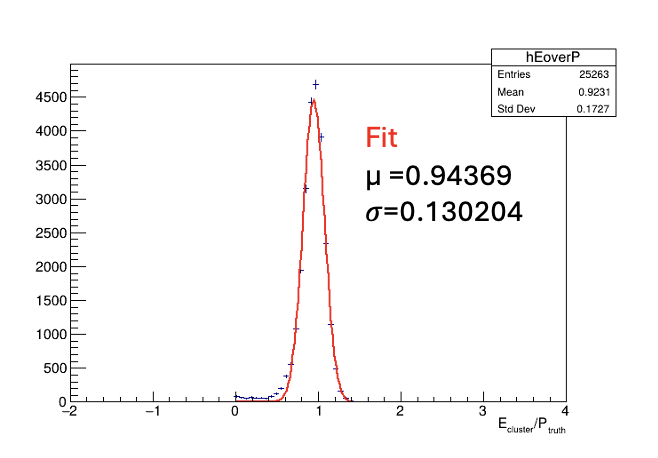
\includegraphics[width=\textwidth]{Figures/topocluster_noise/Resolution_topocluster/ep_3sigma_dr02.png}
    \caption{$3\sigma$}
  \end{subfigure}
  \hfill
  \begin{subfigure}[b]{0.32\textwidth}
    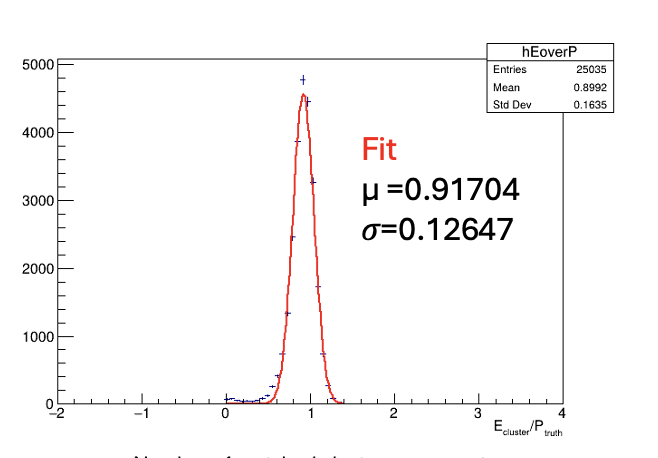
\includegraphics[width=\textwidth]{Figures/topocluster_noise/Resolution_topocluster/ep_4sigma_dr02.png}
    \caption{$4\sigma$}
  \end{subfigure}
  \caption{$E/P$ distributions for electromagnetic particles at $\Delta R < 0.2$ for different noise thresholds.}
  \label{fig:ep_resolution_dr02}
\end{figure}
The resolution of electromagnetic particles at $\Delta R < 0.2$ is found to be 14.1\%, 13.8\%, and 13.8\% for the $2\sigma$, $3\sigma$, and $4\sigma$ noise thresholds, respectively. These values are slightly higher than the corresponding resolutions at $\Delta R < 0.1$, indicating that a tighter matching criterion ($\Delta R < 0.1$) provides better resolution performance for EM clusters.

For hadronic clusters, the resolution is studied under two energy selection criteria: $E > 1$\,GeV and $E > 3$\,GeV. The $E/P$ distributions for hadronic particles matched within $\Delta R < 0.1$ and satisfying $E > 1$\,GeV are shown in Fig.~\ref{fig:ep_hadronic_dr01_e1gev} for the three noise thresholds.

\begin{figure}[h!]
  \centering

  \begin{subfigure}[t]{0.32\textwidth}
    \centering
    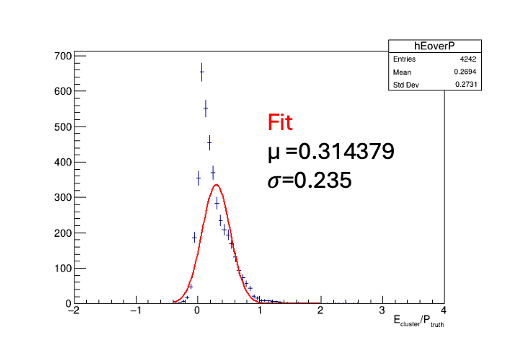
\includegraphics[width=\textwidth]{Figures/topocluster_noise/Resolution_topocluster/ep_hadronic_2sigma_e1gev_dr01.png}
    \caption{$2\sigma$}
  \end{subfigure}
  \hfill
  \begin{subfigure}[t]{0.32\textwidth}
    \centering
    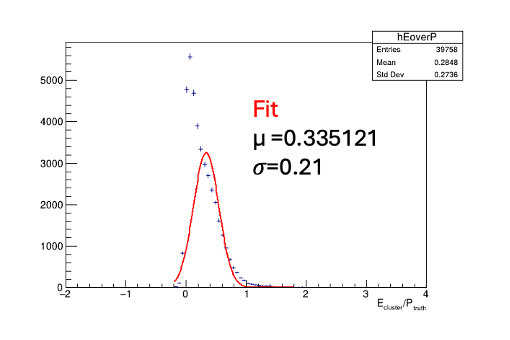
\includegraphics[width=\textwidth]{Figures/topocluster_noise/Resolution_topocluster/ep_hadronic_3sigma_e1gev_dr01.png}
    \caption{$3\sigma$}
  \end{subfigure}
  \hfill
  \begin{subfigure}[t]{0.32\textwidth}
    \centering
    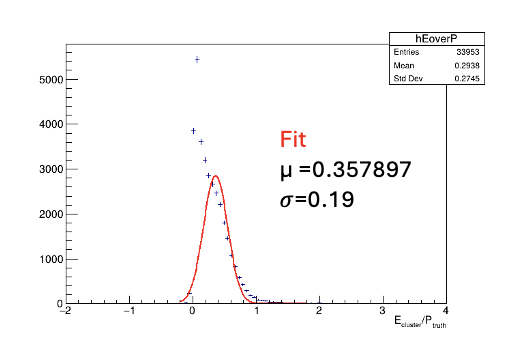
\includegraphics[width=\textwidth]{Figures/topocluster_noise/Resolution_topocluster/ep_hadronic_4sigma_e1gev_dr01.png}
    \caption{$4\sigma$}
  \end{subfigure}

  \caption{$E/P$ distributions for hadronic particles with $E > 1$\,GeV at $\Delta R < 0.1$ for different noise thresholds.}
  \label{fig:ep_hadronic_dr01_e1gev}
\end{figure}

The resolution of hadronic particles under the applied selection criteria ($E > 1$\,GeV and $\Delta R < 0.1$) is found to be 74.75\%, 62.7\%, and 53.1\% for the $2\sigma$, $3\sigma$, and $4\sigma$ noise thresholds, respectively. These results indicate a significant improvement in resolution as the noise suppression becomes stricter.

For the same matching distance ($\Delta R < 0.1$), but with a higher energy threshold ($E > 3$\,GeV), the $E/P$ distributions are also studied for the $1\sigma$, $2\sigma$, and $3\sigma$ noise levels. The corresponding histograms are shown in Fig.~\ref{fig:ep_hadronic_dr01_e3gev}.

\begin{figure}[h!]
  \centering
  \begin{subfigure}[t]{0.32\textwidth}
    \centering
    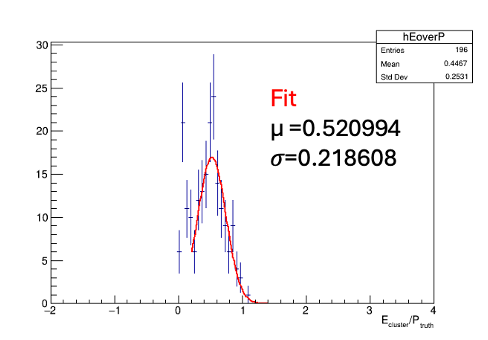
\includegraphics[width=\textwidth]{Figures/topocluster_noise/Resolution_topocluster/ep_hadronic_1sigma_e3gev_dr01.png}
    \caption{$1\sigma$}
  \end{subfigure}
  \hfill
  \begin{subfigure}[t]{0.325\textwidth}
    \centering
    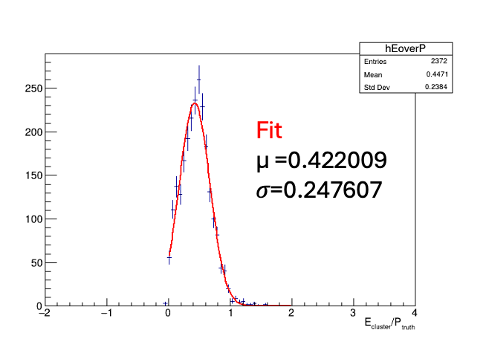
\includegraphics[width=\textwidth]{Figures/topocluster_noise/Resolution_topocluster/ep_hadronic_2sigma_e3gev_dr01.png}
    \caption{$2\sigma$}
  \end{subfigure}
  \hfill
  \begin{subfigure}[t]{0.305\textwidth}
    \centering
    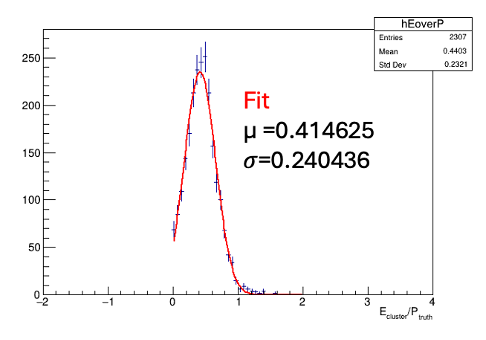
\includegraphics[width=\textwidth]{Figures/topocluster_noise/Resolution_topocluster/ep_hadronic_3sigma_e3gev_dr01.png}
    \caption{$3\sigma$}
  \end{subfigure}
  \caption{$E/P$ distributions for hadronic particles with $E > 3$\,GeV at $\Delta R < 0.1$ for different noise thresholds ($1\sigma$, $2\sigma$, and $3\sigma$).}
  \label{fig:ep_hadronic_dr01_e3gev}
\end{figure}

The resolutions extracted from the $E/P$ distributions for hadronic particles with $E > 3$\,GeV and $\Delta R < 0.1$ are 42.0\%, 58.7\%, and 58.0\% for the $2\sigma$, $3\sigma$, and $4\sigma$ noise thresholds, respectively. These values indicate an improved resolution compared to the lower energy case with $E > 1$\,GeV and are broadly consistent with test beam expectations. However, due to the more stringent energy selection, the reduced number of matched events results in larger statistical fluctuations in the distributions.

Additionally, the $E/P$ distributions for hadronic topoclusters matched within $\Delta R < 0.2$ and satisfying $E > 1$\,GeV are shown in Fig.~\ref{fig:ep_hadronic_dr02_e1gev}. These provide insight into the resolution behavior under a looser spatial matching condition.

\begin{figure}[h!]
  \centering
  \begin{subfigure}[b]{0.32\textwidth}
    \centering
    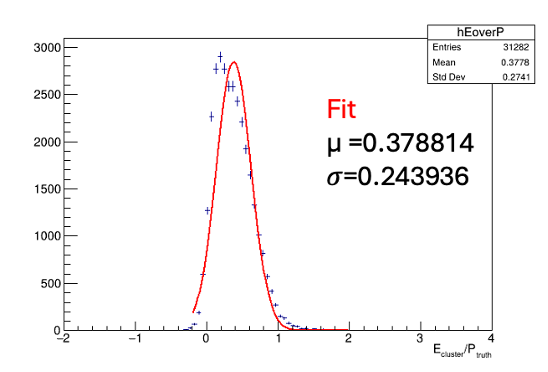
\includegraphics[width=\textwidth]{Figures/topocluster_noise/Resolution_topocluster/ep_hadronic_2sigma_e1gev_dr02.png}
    \caption{$2\sigma$}
  \end{subfigure}
  \hfill
  \begin{subfigure}[b]{0.32\textwidth}
    \centering
    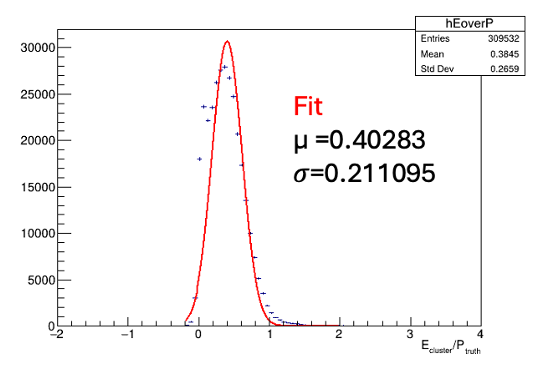
\includegraphics[width=\textwidth]{Figures/topocluster_noise/Resolution_topocluster/ep_hadronic_3sigma_e1gev_dr02.png}
    \caption{$3\sigma$}
  \end{subfigure}
  \hfill
  \begin{subfigure}[b]{0.32\textwidth}
    \centering
    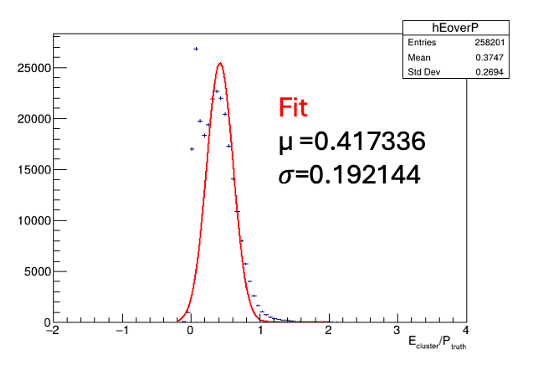
\includegraphics[width=\textwidth]{Figures/topocluster_noise/Resolution_topocluster/ep_hadronic_4sigma_e1gev_dr02.png}
    \caption{$4\sigma$}
  \end{subfigure}
  \caption{$E/P$ distributions for hadronic particles with $E > 1$\,GeV at $\Delta R < 0.2$ for different noise thresholds.}
  \label{fig:ep_hadronic_dr02_e1gev}
\end{figure}
The resolutions extracted from the $E/P$ distributions for hadronic particles with $E > 1$\,GeV and matched within $\Delta R < 0.2$ are found to be 64.4\%, 52.4\%, and 46.0\% for the $2\sigma$, $3\sigma$, and $4\sigma$ noise thresholds, respectively. Compared to the corresponding results at $\Delta R < 0.1$, the resolutions are slightly degraded, as expected due to the looser spatial matching criterion. Nevertheless, a consistent trend of improved resolution with stronger noise suppression is observed, confirming the robustness of the topocluster reconstruction performance under varying spatial and noise conditions.
The $E/P$ distributions for hadronic particles with $E > 3$\,GeV and matched within $\Delta R < 0.2$ are shown in Fig.~\ref{fig:ep_hadronic_dr02_e3gev} for the $2\sigma$, $3\sigma$, and $4\sigma$ noise thresholds.

\begin{figure}[h!]
  \centering
  \begin{subfigure}[b]{0.32\textwidth}
    \centering
    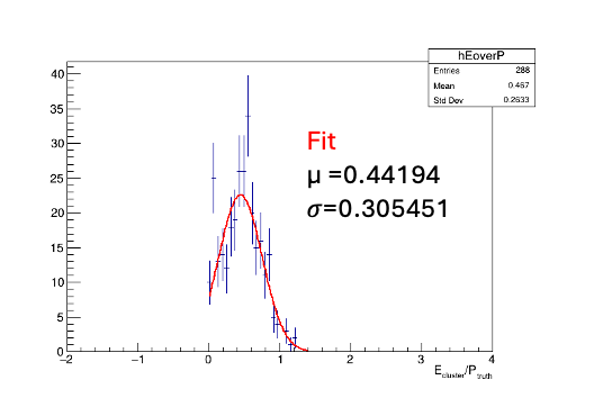
\includegraphics[width=\textwidth]{Figures/topocluster_noise/Resolution_topocluster/ep_hadronic_2sigma_e3gev_dr02.png}
    \caption{$2\sigma$}
  \end{subfigure}
  \hfill
  \begin{subfigure}[b]{0.32\textwidth}
    \centering
    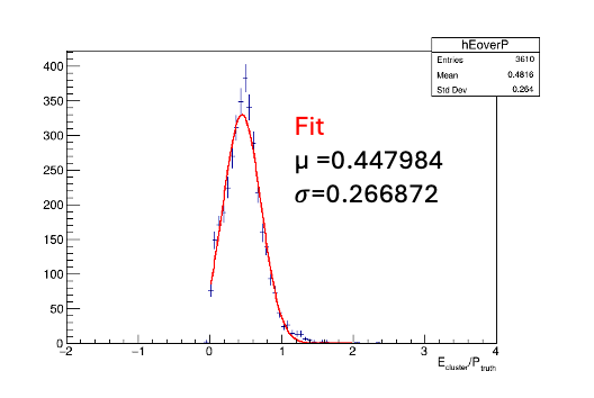
\includegraphics[width=\textwidth]{Figures/topocluster_noise/Resolution_topocluster/ep_hadronic_3sigma_e3gev_dr02.png}
    \caption{$3\sigma$}
  \end{subfigure}
  \hfill
  \begin{subfigure}[b]{0.32\textwidth}
    \centering
    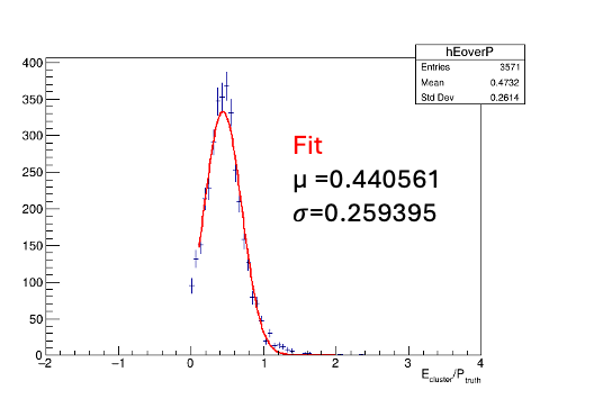
\includegraphics[width=\textwidth]{Figures/topocluster_noise/Resolution_topocluster/ep_hadronic_4sigma_e3gev_dr02.png}
    \caption{$4\sigma$}
  \end{subfigure}
  \caption{$E/P$ distributions for hadronic particles with $E > 3$\,GeV at $\Delta R < 0.2$ for different noise thresholds.}
  \label{fig:ep_hadronic_dr02_e3gev}
\end{figure}

The extracted resolutions for hadronic particles under these conditions are found to be 69.1\%, 59.6\%, and 58.9\% for the $2\sigma$, $3\sigma$, and $4\sigma$ thresholds, respectively. These results are notably worse than the corresponding values obtained at $\Delta R < 0.1$, indicating a degradation in resolution performance when a looser spatial matching criterion is applied. This behavior highlights the importance of a tighter $\Delta R$ requirement for improving the energy resolution of topoclusters, even at higher energy thresholds. Despite the higher $E$ cut, the broader matching radius introduces more contamination or mismatches, leading to increased fluctuations in the $E/P$ distribution.
A comparison across all configurations shows that the $2\sigma$ noise threshold consistently yields the worst energy resolution for hadronic particles. In contrast, the resolutions obtained with the $3\sigma$ and $4\sigma$ thresholds are significantly better and are found to be very similar to each other in most cases. Based on this observation, the $3\sigma$ threshold is selected as the optimal working point, balancing resolution performance and noise suppression.

To further enhance the resolution—especially for hadronic particles—track–calorimeter matching techniques are applied. This study is performed using the $3\sigma$ noise threshold and selecting clusters with $E > 3$\,GeV. Two matching distances, $\Delta R < 0.1$ and $\Delta R < 0.2$, are considered. The applied tracking cuts include:  
(i) an isolation requirement where no other truth particles with $p_T > 0.2$\,GeV exist within $\Delta R < 0.6$ of the target truth particle,  
(ii) a transverse momentum threshold of $p_T > 3$\,GeV for the truth particle, and  
(iii) a longitudinal position constraint of $|z| < 10$\,cm.  
These criteria aim to ensure clean and well-reconstructed matches between truth particles and calorimeter clusters, providing a more accurate estimate of the topocluster energy resolution.
The figures below show the $E/P$ distributions for hadronic particles with $E > 3$\,GeV and matched within $\Delta R < 0.2$, for events where the corresponding track is associated with hits in the EMCal, IHCal, and OHCal layers, respectively. These distributions allow for a more detailed assessment of the calorimeter response in different detector regions.

\begin{figure}[h!]
  \centering
  \begin{subfigure}[b]{0.32\textwidth}
    \centering
    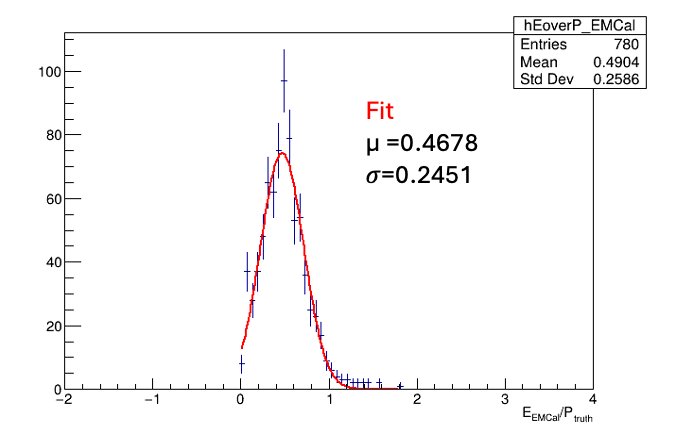
\includegraphics[width=\textwidth]{Figures/topocluster_noise/Resolution_topocluster/ep_trackmatched_emcal.png}
    \caption{EMCal}
  \end{subfigure}
  \hfill
  \begin{subfigure}[b]{0.32\textwidth}
    \centering
    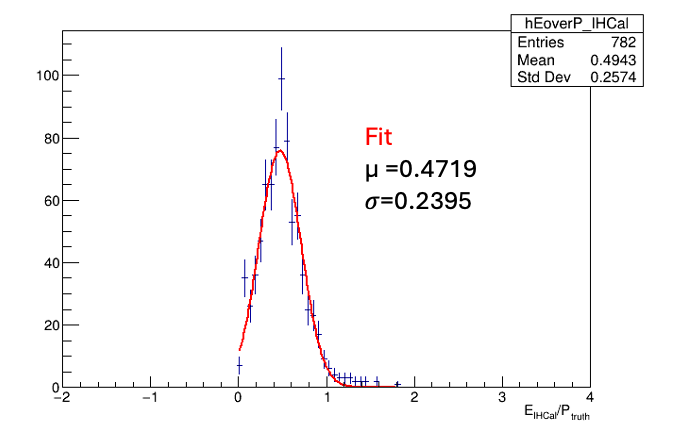
\includegraphics[width=\textwidth]{Figures/topocluster_noise/Resolution_topocluster/ep_trackmatched_ihcal.png}
    \caption{IHCal}
  \end{subfigure}
  \hfill
  \begin{subfigure}[b]{0.32\textwidth}
    \centering
    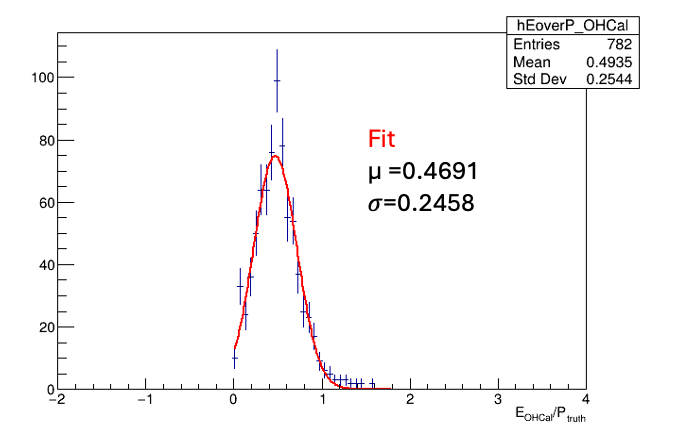
\includegraphics[width=\textwidth]{Figures/topocluster_noise/Resolution_topocluster/ep_trackmatched_ohcal.png}
    \caption{OHCal}
  \end{subfigure}
  \caption{$E/P$ distributions for hadronic particles with $E > 3$\,GeV and $\Delta R < 0.2$, where the matched track has hits in the EMCal, IHCal, and OHCal calorimeter layers.}
  \label{fig:ep_trackmatched_calolayers}
\end{figure}
In this study, the cluster energy is computed starting from the calorimeter face where the matched track first enters the calorimeter system. Specifically, $E_{\mathrm{EMCal}}$, $E_{\mathrm{IHCal}}$, and $E_{\mathrm{OHCal}}$ represent the energy of the topocluster components beginning at the EMCal, IHCal, and OHCal front faces, respectively, depending on where the track intersects the detector. This approach allows for a more localized energy measurement based on the particle’s entry point.
The resulting energy resolution, calculated using this track-based selection and summing method, is found to be 51\%. This represents a significant improvement over the inclusive hadronic resolution observed for $\Delta R < 0.2$ without track–calorimeter matching, highlighting the benefit of incorporating tracking information in calorimeter-based energy measurements.
A similar study is performed using a tighter spatial matching requirement of $\Delta R < 0.1$ and an energy threshold of $E > 3$\,GeV. As before, the cluster energy is computed based on the calorimeter face where the matched track first enters (EMCal, IHCal, or OHCal). The corresponding $E/P$ distributions are shown in Fig.~\ref{fig:ep_trackmatched_dr01}.

\begin{figure}[h!]
  \centering
  \begin{subfigure}[b]{0.32\textwidth}
    \centering
    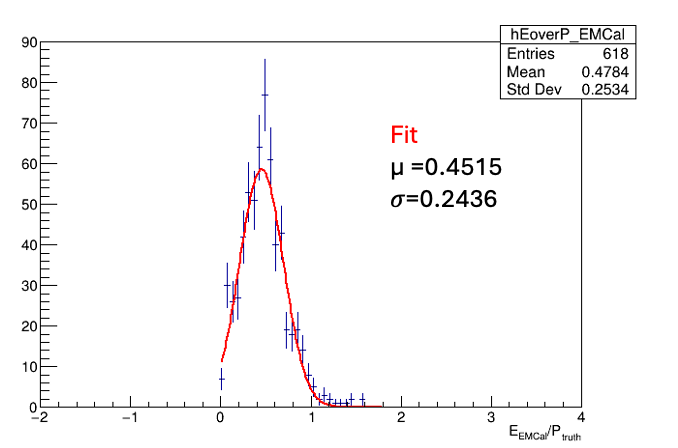
\includegraphics[width=\textwidth]{Figures/topocluster_noise/Resolution_topocluster/ep_trackmatched_emcal_dr01.png}
    \caption{EMCal}
  \end{subfigure}
  \hfill
  \begin{subfigure}[b]{0.32\textwidth}
    \centering
    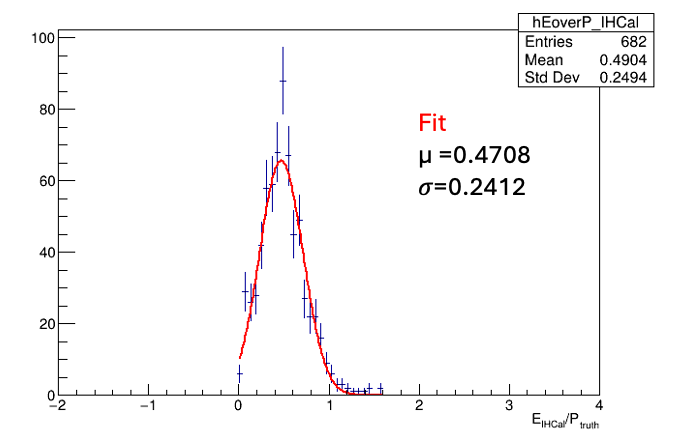
\includegraphics[width=\textwidth]{Figures/topocluster_noise/Resolution_topocluster/ep_trackmatched_ihcal_dr01.png}
    \caption{IHCal}
  \end{subfigure}
  \hfill
  \begin{subfigure}[b]{0.32\textwidth}
    \centering
    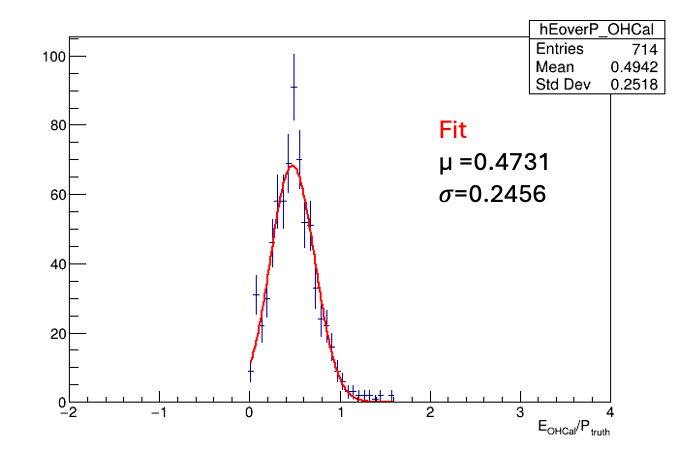
\includegraphics[width=\textwidth]{Figures/topocluster_noise/Resolution_topocluster/ep_trackmatched_ohcal_dr01.png}
    \caption{OHCal}
  \end{subfigure}
  \caption{$E/P$ distributions for hadronic particles with $E > 3$\,GeV and $\Delta R < 0.1$, where the matched track has hits in the EMCal, IHCal, and OHCal calorimeter layers.}
  \label{fig:ep_trackmatched_dr01}
\end{figure}
The extracted resolution for this configuration is found to be 52\%. Compared to the $\Delta R < 0.2$ case, this result does not show an improvement, which can be attributed to the deeper and more diffuse shower development of hadronic particles. A tighter matching cone may exclude relevant energy deposits, leading to a slight degradation in resolution despite the use of track-based calorimeter localization.
Another configuration studied involves hadronic particles with $E > 1$\,GeV and $\Delta R < 0.2$, using track–calorimeter matching. The $E/P$ distributions for tracks intersecting the EMCal, IHCal, and OHCal front faces are shown in Fig.~\ref{fig:ep_trackmatched_e1gev_dr02}.

\begin{figure}[h!]
  \centering
  \begin{subfigure}[b]{0.32\textwidth}
    \centering
    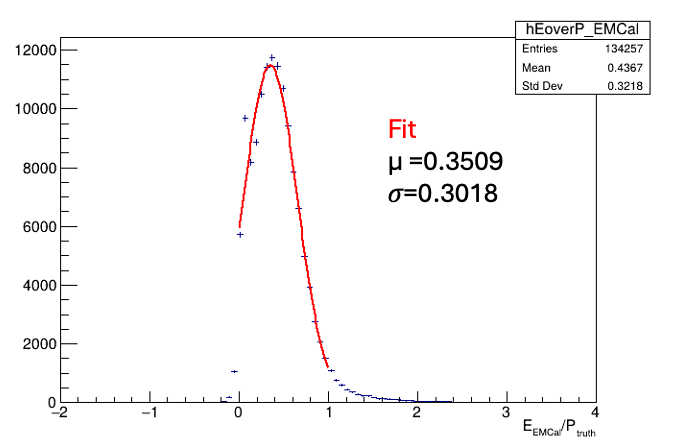
\includegraphics[width=\textwidth]{Figures/topocluster_noise/Resolution_topocluster/ep_trackmatched_emcal_e1gev_dr02.png}
    \caption{EMCal}
  \end{subfigure}
  \hfill
  \begin{subfigure}[b]{0.32\textwidth}
    \centering
    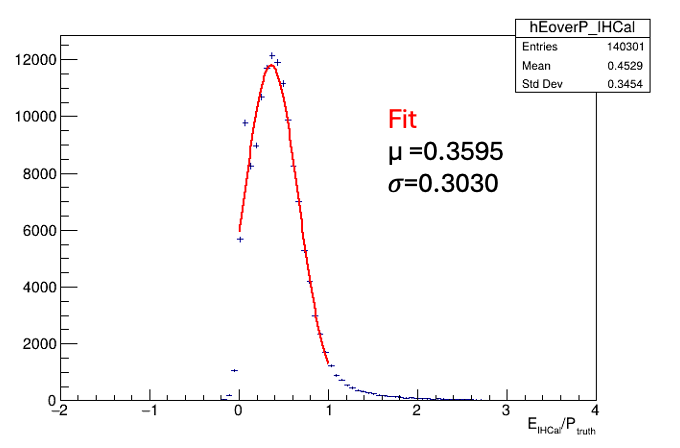
\includegraphics[width=\textwidth]{Figures/topocluster_noise/Resolution_topocluster/ep_trackmatched_ihcal_e1gev_dr02.png}
    \caption{IHCal}
  \end{subfigure}
  \hfill
  \begin{subfigure}[b]{0.32\textwidth}
    \centering
    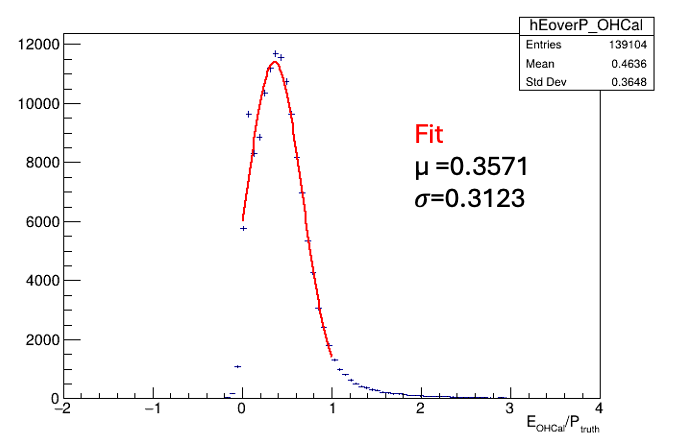
\includegraphics[width=\textwidth]{Figures/topocluster_noise/Resolution_topocluster/ep_trackmatched_ohcal_e1gev_dr02.png}
    \caption{OHCal}
  \end{subfigure}
  \caption{$E/P$ distributions for hadronic particles with $E > 1$\,GeV and $\Delta R < 0.2$, where the matched track has hits in the EMCal, IHCal, and OHCal calorimeter layers.}
  \label{fig:ep_trackmatched_e1gev_dr02}
\end{figure}

The extracted resolution in this configuration is found to be 84\%, which is significantly worse than in the higher-energy cases. This degradation is expected, as 1\,GeV hadrons often do not fully penetrate the hadronic calorimeter, resulting in incomplete shower containment and underestimation of the total deposited energy. The calorimeter’s sampling and interaction depth are not optimized for such low-energy hadrons, which leads to large fluctuations in the $E/P$ response.
The configuration with $E > 1$\,GeV and $\Delta R < 0.1$ is also examined using track–calorimeter matching. The $E/P$ distributions corresponding to tracks that intersect the EMCal, IHCal, and OHCal front faces are shown in Fig.~\ref{fig:ep_trackmatched_e1gev_dr01}.

\begin{figure}[h!]
  \centering
  \begin{subfigure}[b]{0.32\textwidth}
    \centering
    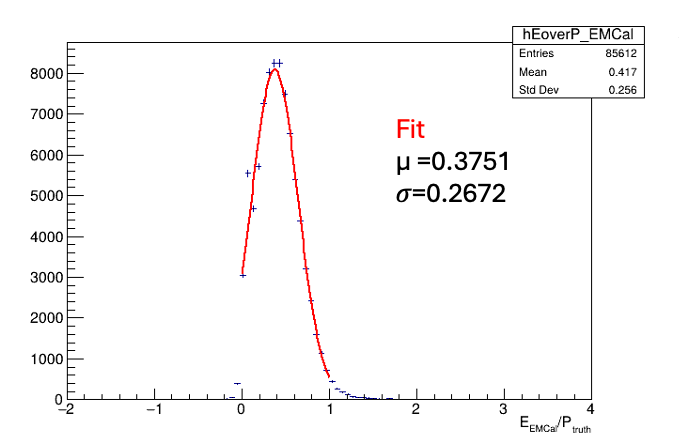
\includegraphics[width=\textwidth]{Figures/topocluster_noise/Resolution_topocluster/ep_trackmatched_emcal_e1gev_dr01.png}
    \caption{EMCal}
  \end{subfigure}
  \hfill
  \begin{subfigure}[b]{0.32\textwidth}
    \centering
    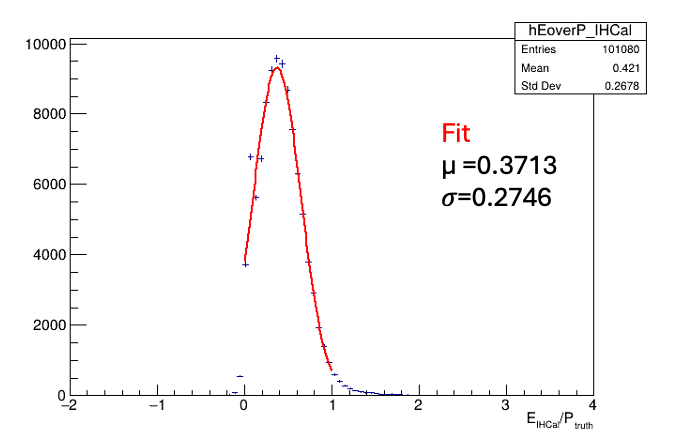
\includegraphics[width=\textwidth]{Figures/topocluster_noise/Resolution_topocluster/ep_trackmatched_ihcal_e1gev_dr01.png}
    \caption{IHCal}
  \end{subfigure}
  \hfill
  \begin{subfigure}[b]{0.32\textwidth}
    \centering
    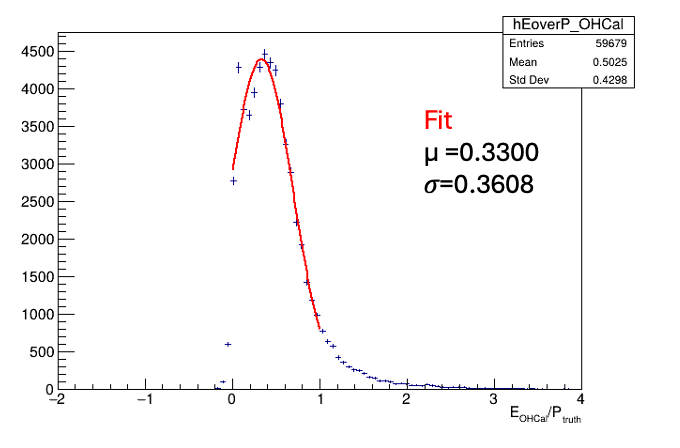
\includegraphics[width=\textwidth]{Figures/topocluster_noise/Resolution_topocluster/ep_trackmatched_ohcal_e1gev_dr01.png}
    \caption{OHCal}
  \end{subfigure}
  \caption{$E/P$ distributions for hadronic particles with $E > 1$\,GeV and $\Delta R < 0.1$, where the matched track has hits in the EMCal, IHCal, and OHCal calorimeter layers.}
  \label{fig:ep_trackmatched_e1gev_dr01}
\end{figure}

The extracted resolution in this case is 73\%, as shown in Fig.~\ref{fig:ep_trackmatched_e1gev_dr01}. This result shows a moderate improvement compared to the $\Delta R < 0.2$ case (84\%), due to the tighter spatial matching requirement. By limiting the matching radius, the contribution from nearby noise or overlapping showers is reduced, resulting in slightly better containment and cleaner association between the track and the corresponding topocluster.
Overall, the best resolution is observed for hadronic particles with $E > 3$\,GeV and $\Delta R < 0.2$, reaching 51\% with track–calorimeter matching. This performance is consistent with expectations from test beam measurements, further validating the use of this configuration as the optimal working point for precision calorimetric reconstruction.




\subsubsection{UE from towers versus topoclusters}
The reconstructed transverse energy in dijet events from summing calorimeter towers versus summing topoclusters are shown in Figure~\ref{fig:towers_and_topo} with the updated noise thresholds for the topocluster seeding. The \ET{} from towers is wider and was foudn to be highly dependent on the reconstruction method and noise contributions (see Section~\ref{sec:initial_studies}) while the \ET{} from topoclusters is much less dependent on the reconstruction method and noise level. Notably, the mean topocluster \ET{} in the transverse region is about half the tower sum \ET{} in the transverse region, meaning likely the towers measurement contains a large noise contribution. This information combined with the robustness of the topoclusters to noise and caloriemter reconstruction seen in Section~\ref{sec:initial_studies} makes using the topoclusters with optimized noise thresholds, the best choice for this measurement. 

\begin{figure}[h!]
    \centering
    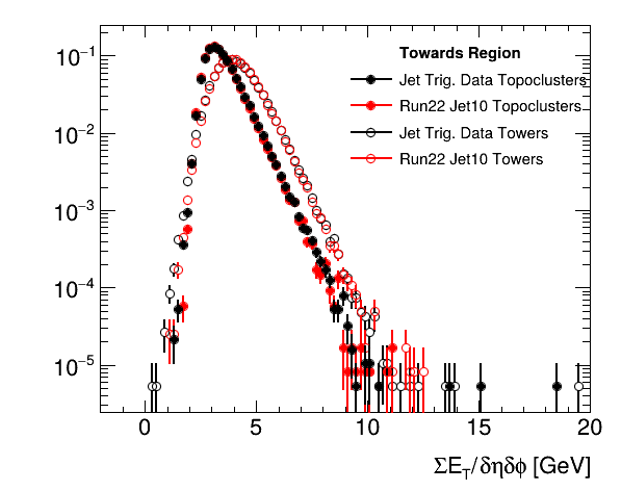
\includegraphics[width=0.32\linewidth]{Figures/topocluster_noise/towards_ET.png}
    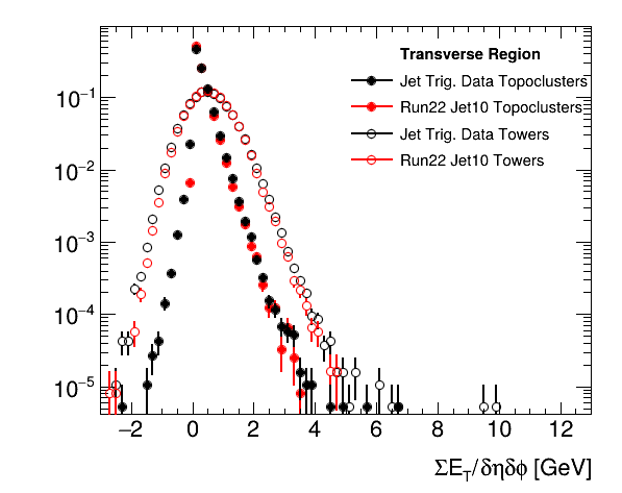
\includegraphics[width=0.32\linewidth]{Figures/topocluster_noise/transverse_ET.png}
    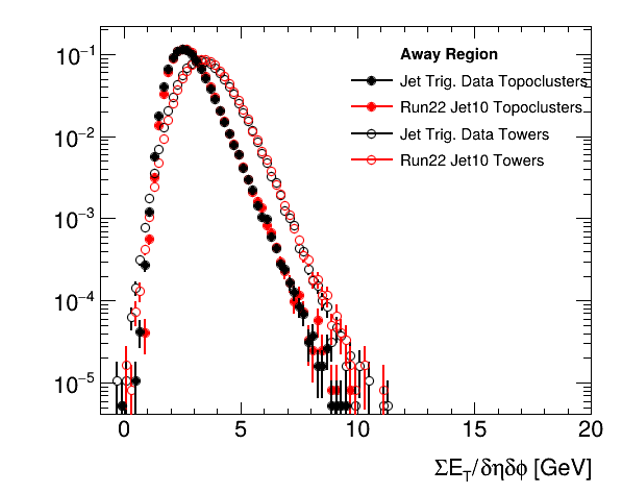
\includegraphics[width=0.32\linewidth]{Figures/topocluster_noise/away_ET.png}
    \caption{Comparison of towards, transverse and away region energy distributions from topoclusters (solid points) and towers (hollow points) in dijet events using ana468p012\_v001 data (black) and Run 22 Jet 10 simulation (red) datasets.}
    \label{fig:towers_and_topo}
\end{figure}

\subsubsection{UE from Towers QA}\label{sec:UE_from_Towers_QA}
Comparisons of tower energy spectra in transverse UE revealed an excess of events with an OHCal tower having an abnormally negative energy value in data relative to simulation. Figure~\ref{fig:UE_spectra_sim_vs_49219} shows the comparison of these spectra from a single Run 49219 in data to the 10 GeV Run 21 simulation. A total of 66 events were found in Run 49219 that contained an OHCal tower with E$_T <$ --3 GeV. These event numbers were collected and the waveforms of the OHCal towers were inspected for irregularities. Since the data was zero-suppressed, only the ADC values for time samples 0 and 6 were saved in the calorimeter DST files rather than the entire waveform. It was discovered that the waveforms of these towers had a large ADC at time sample 0 and an ADC consistent with pedestal levels at sample 6, where the signal would be expected. This could be consistent with the triggered event being in the adjacent bunch crossing immediately after a collision.

\begin{figure}[h!]
    \centering
    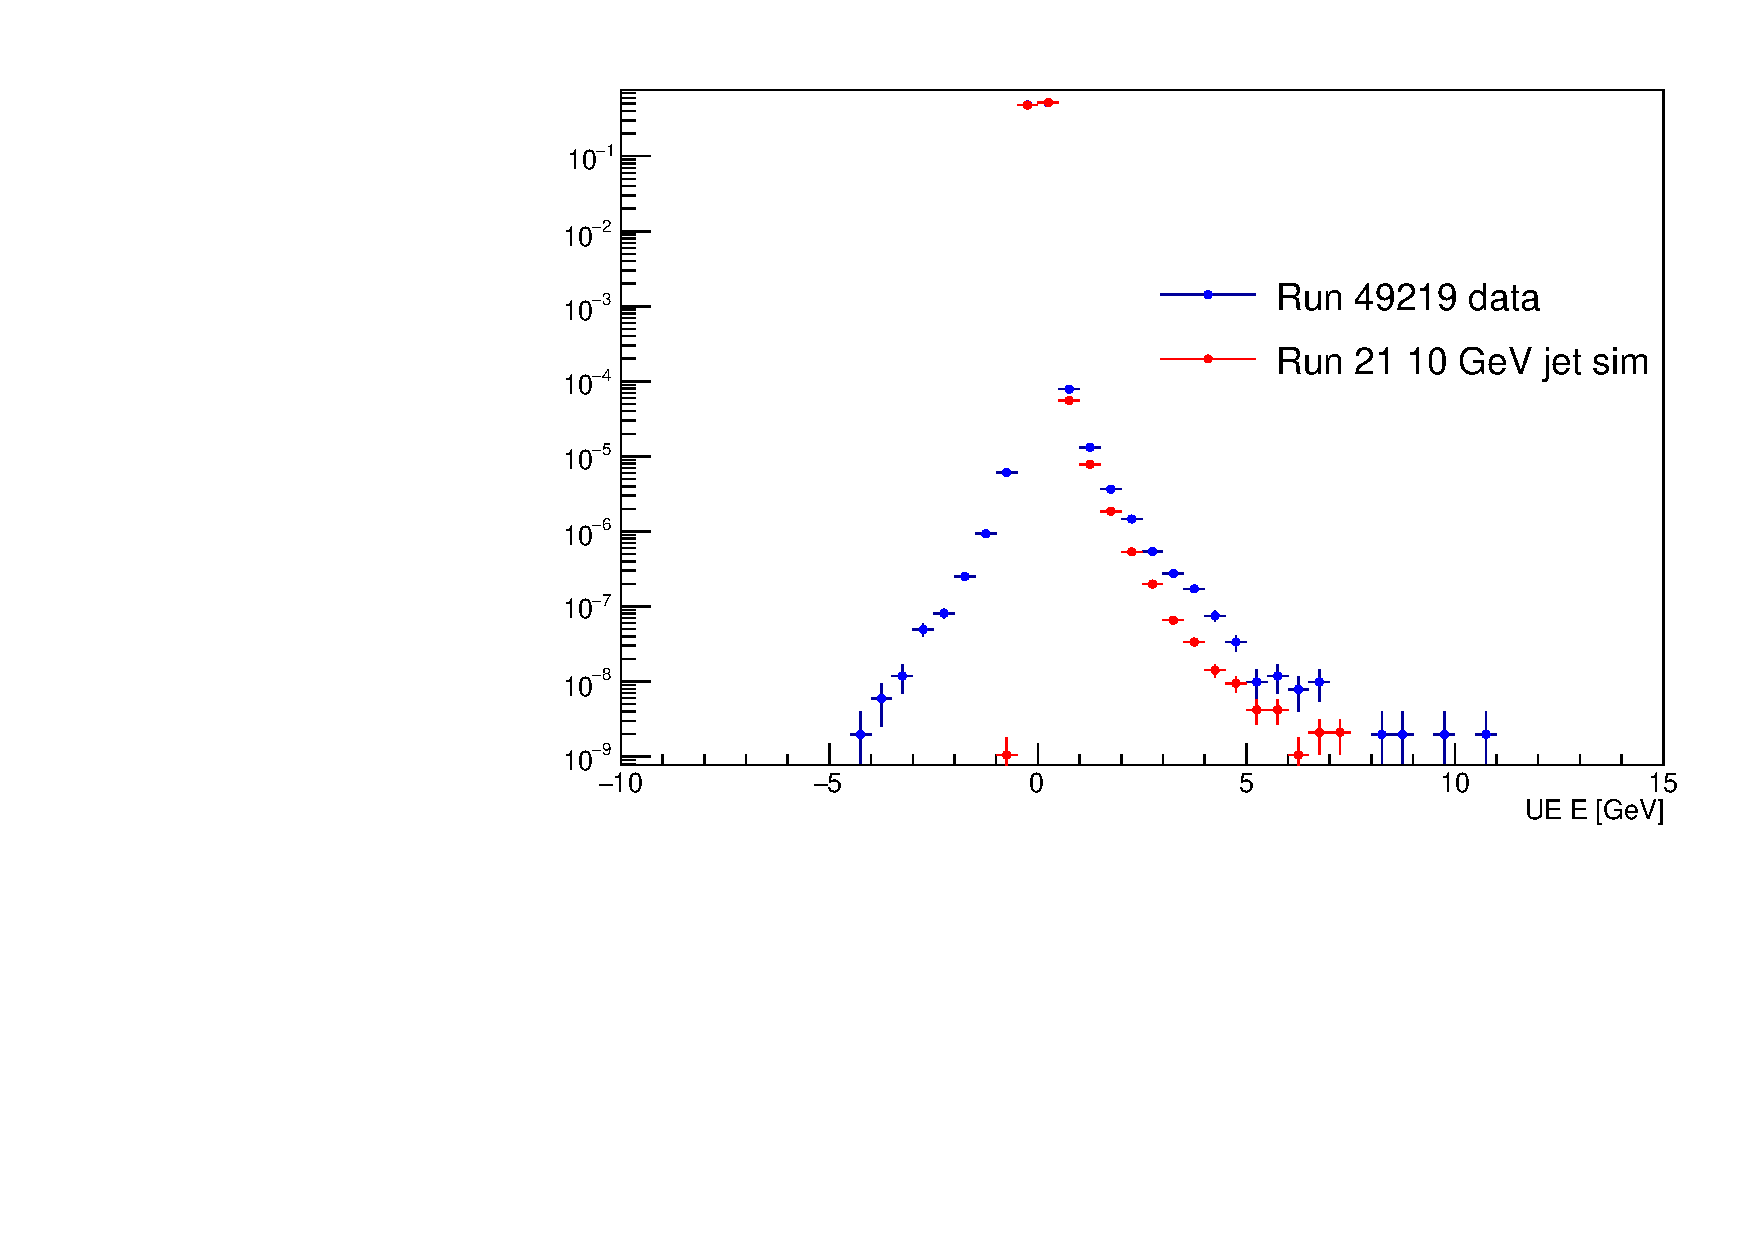
\includegraphics[width=0.5\linewidth]{Figures/mbd_waveforms_pileup/UE_spectra_sim_vs_49219.pdf}
    \caption{Transverse UE tower energy spectra for Run 49219 in data (blue) and Run 21 simulation (red).}
    \label{fig:UE_spectra_sim_vs_49219}
\end{figure}

To test if these very negative UE towers are in fact the result of out-of-time pileup, the MBD waveforms were plotted for 12 of the 66 events having an OHCal tower with energy below --3 GeV. A typical event will have an MBD waveform with a single peak around time sample 8, but an event with out-of-time pileup will contain more than one peak in its waveform. The MBD has 64 arms on each the North and South side, so all 128 waveforms were plotted together in a 2D histogram for simplicity. Fig.~\ref{fig:MBD_2D_waveforms} shows these waveforms and their corresponding event numbers. It is immediately apparent from these 2D waveforms that each of these 12 events were triggered on a bunch crossing directly after a crossing that contained a collision.

\begin{figure}[h!]
    \centering
    \begin{subfigure}{.329\textwidth}
    \centering
      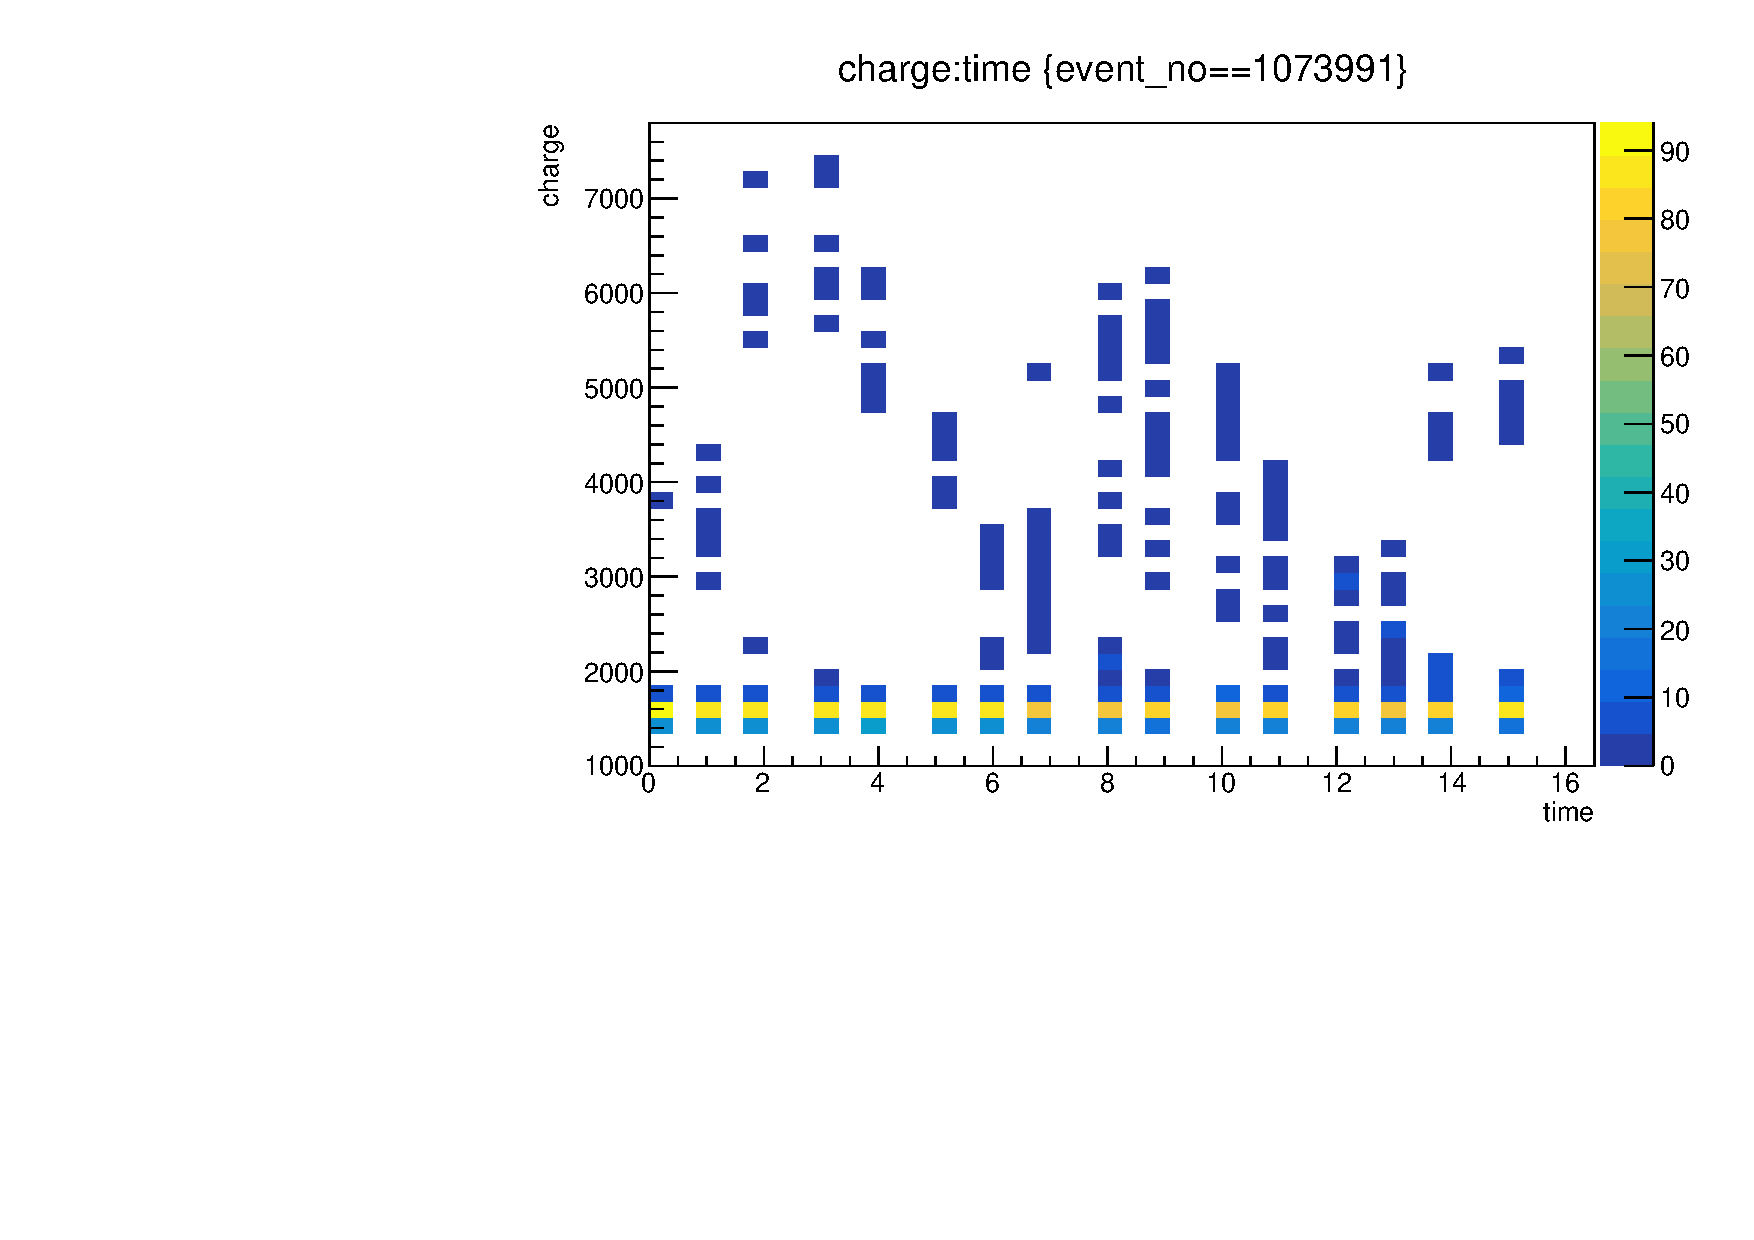
\includegraphics[width=1.\textwidth]{Figures/mbd_waveforms_pileup/MBD_2D_evt1073991.pdf}
    \end{subfigure}
    \begin{subfigure}{.329\textwidth}
    \centering
        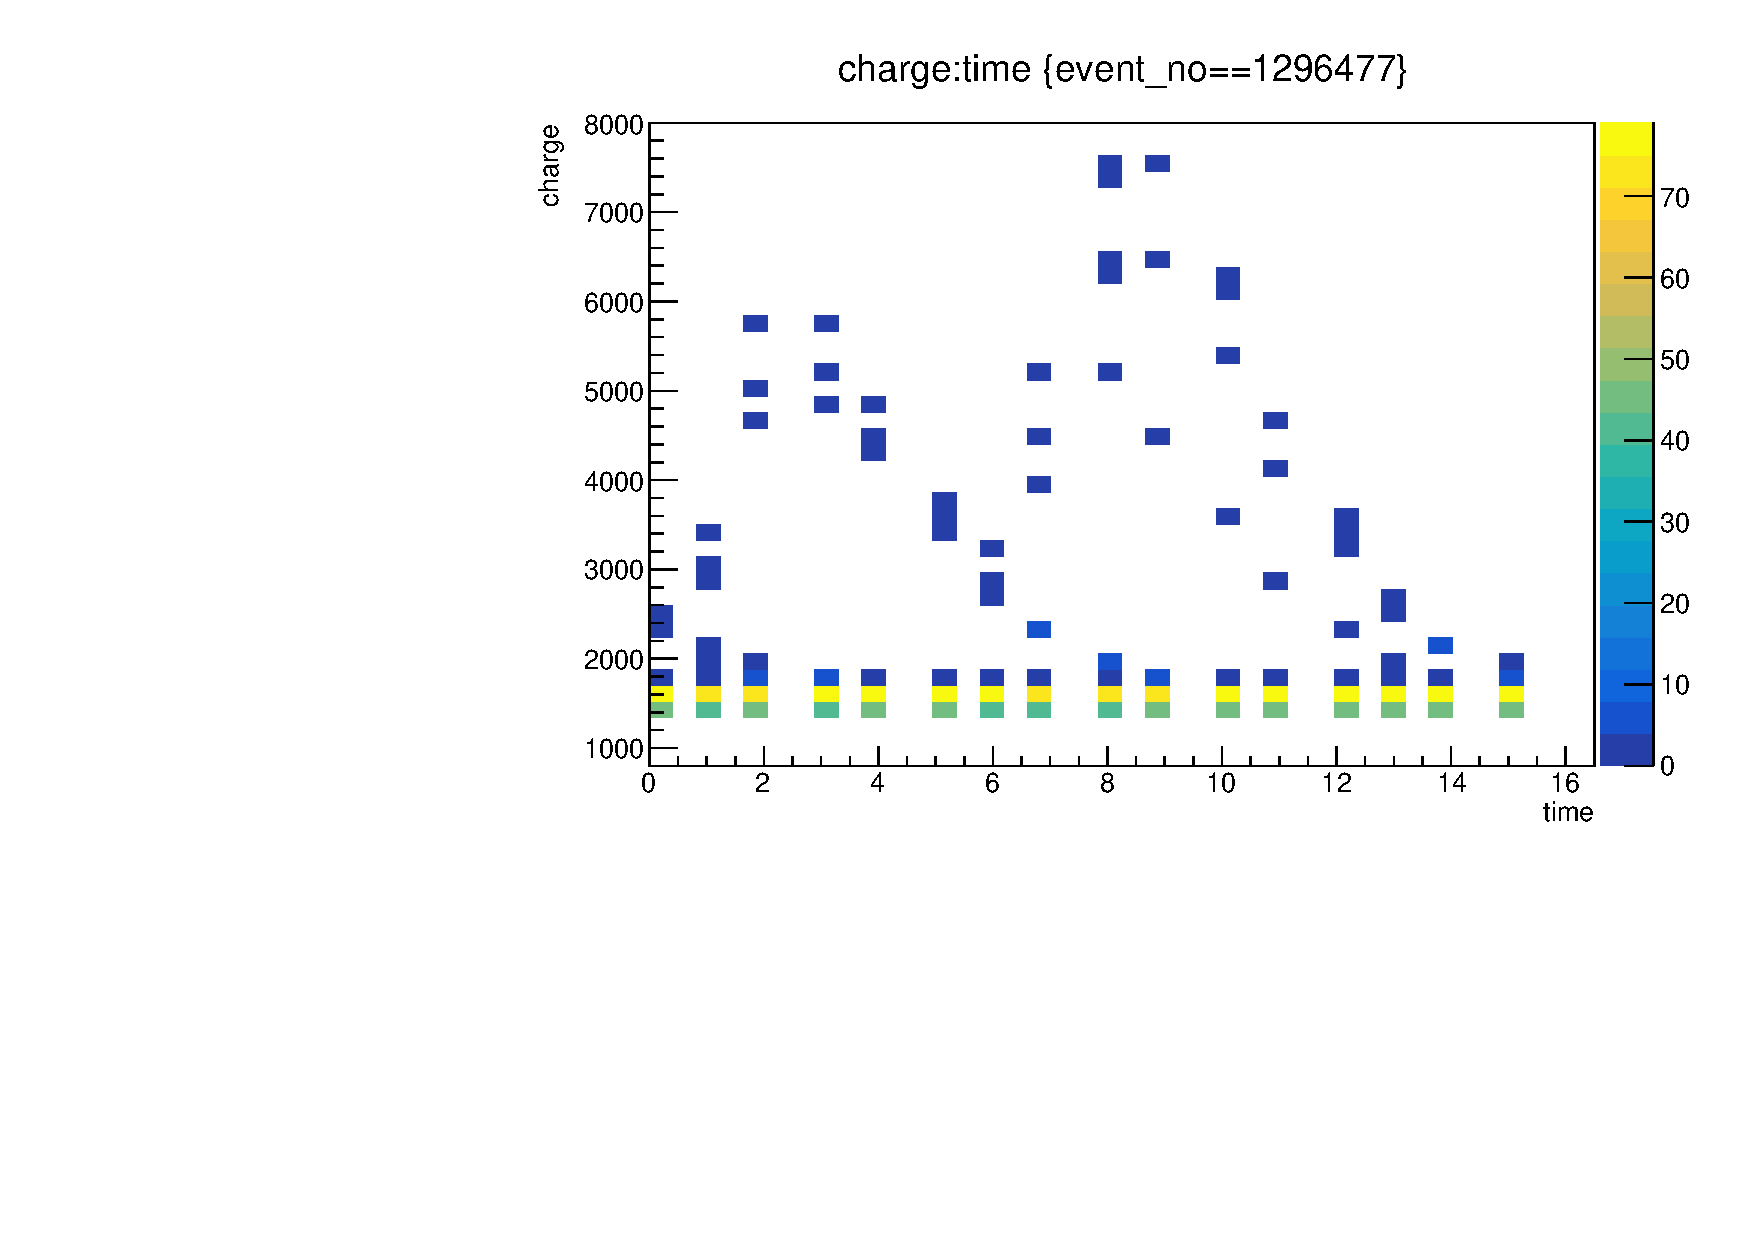
\includegraphics[width=1.\textwidth]{Figures/mbd_waveforms_pileup/MBD_2D_evt1296477.pdf}
    \end{subfigure}
    \begin{subfigure}{.329\textwidth}
    \centering
        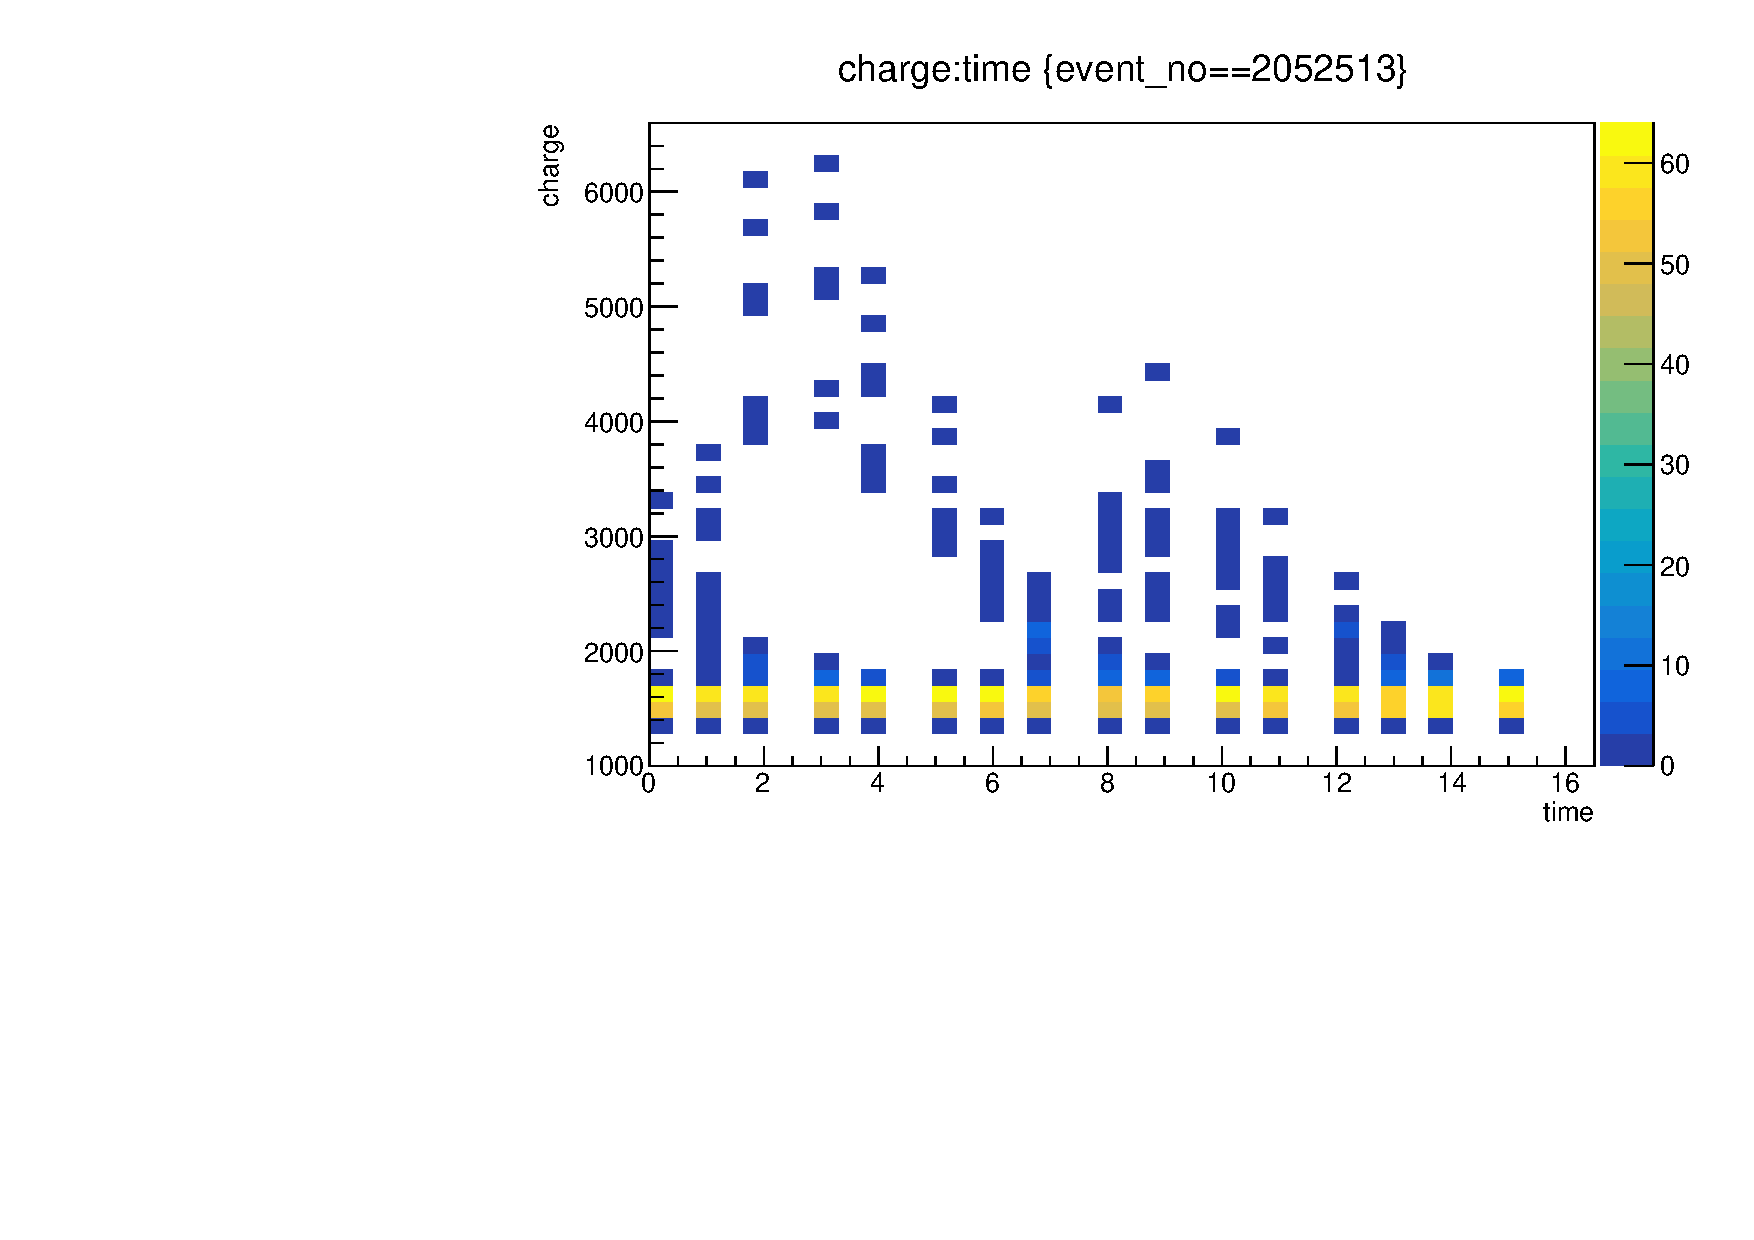
\includegraphics[width=1.\textwidth]{Figures/mbd_waveforms_pileup/MBD_2D_evt2052513.pdf}
    \end{subfigure}

    \begin{subfigure}{.329\textwidth}
    \centering
      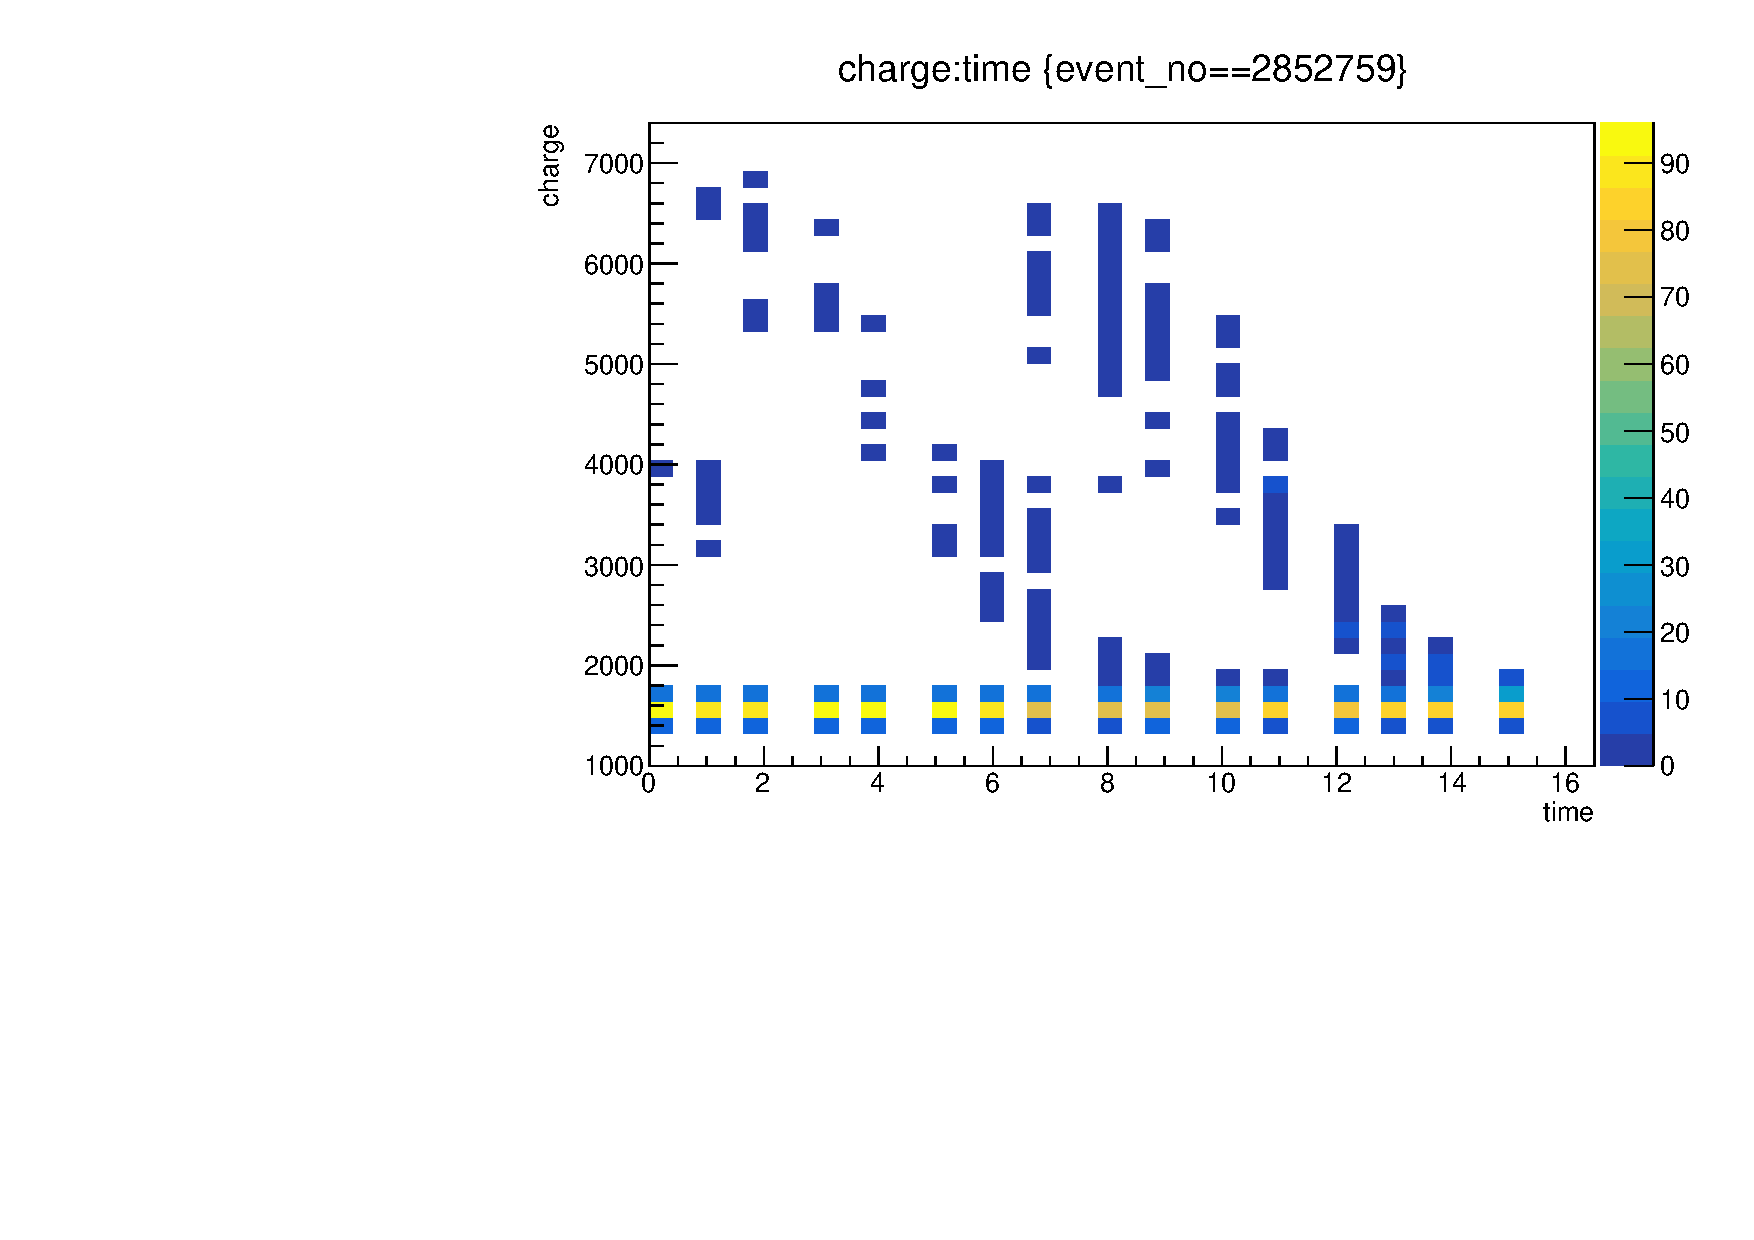
\includegraphics[width=1.\textwidth]{Figures/mbd_waveforms_pileup/MBD_2D_evt2852759.pdf}
    \end{subfigure}
    \begin{subfigure}{.329\textwidth}
    \centering
        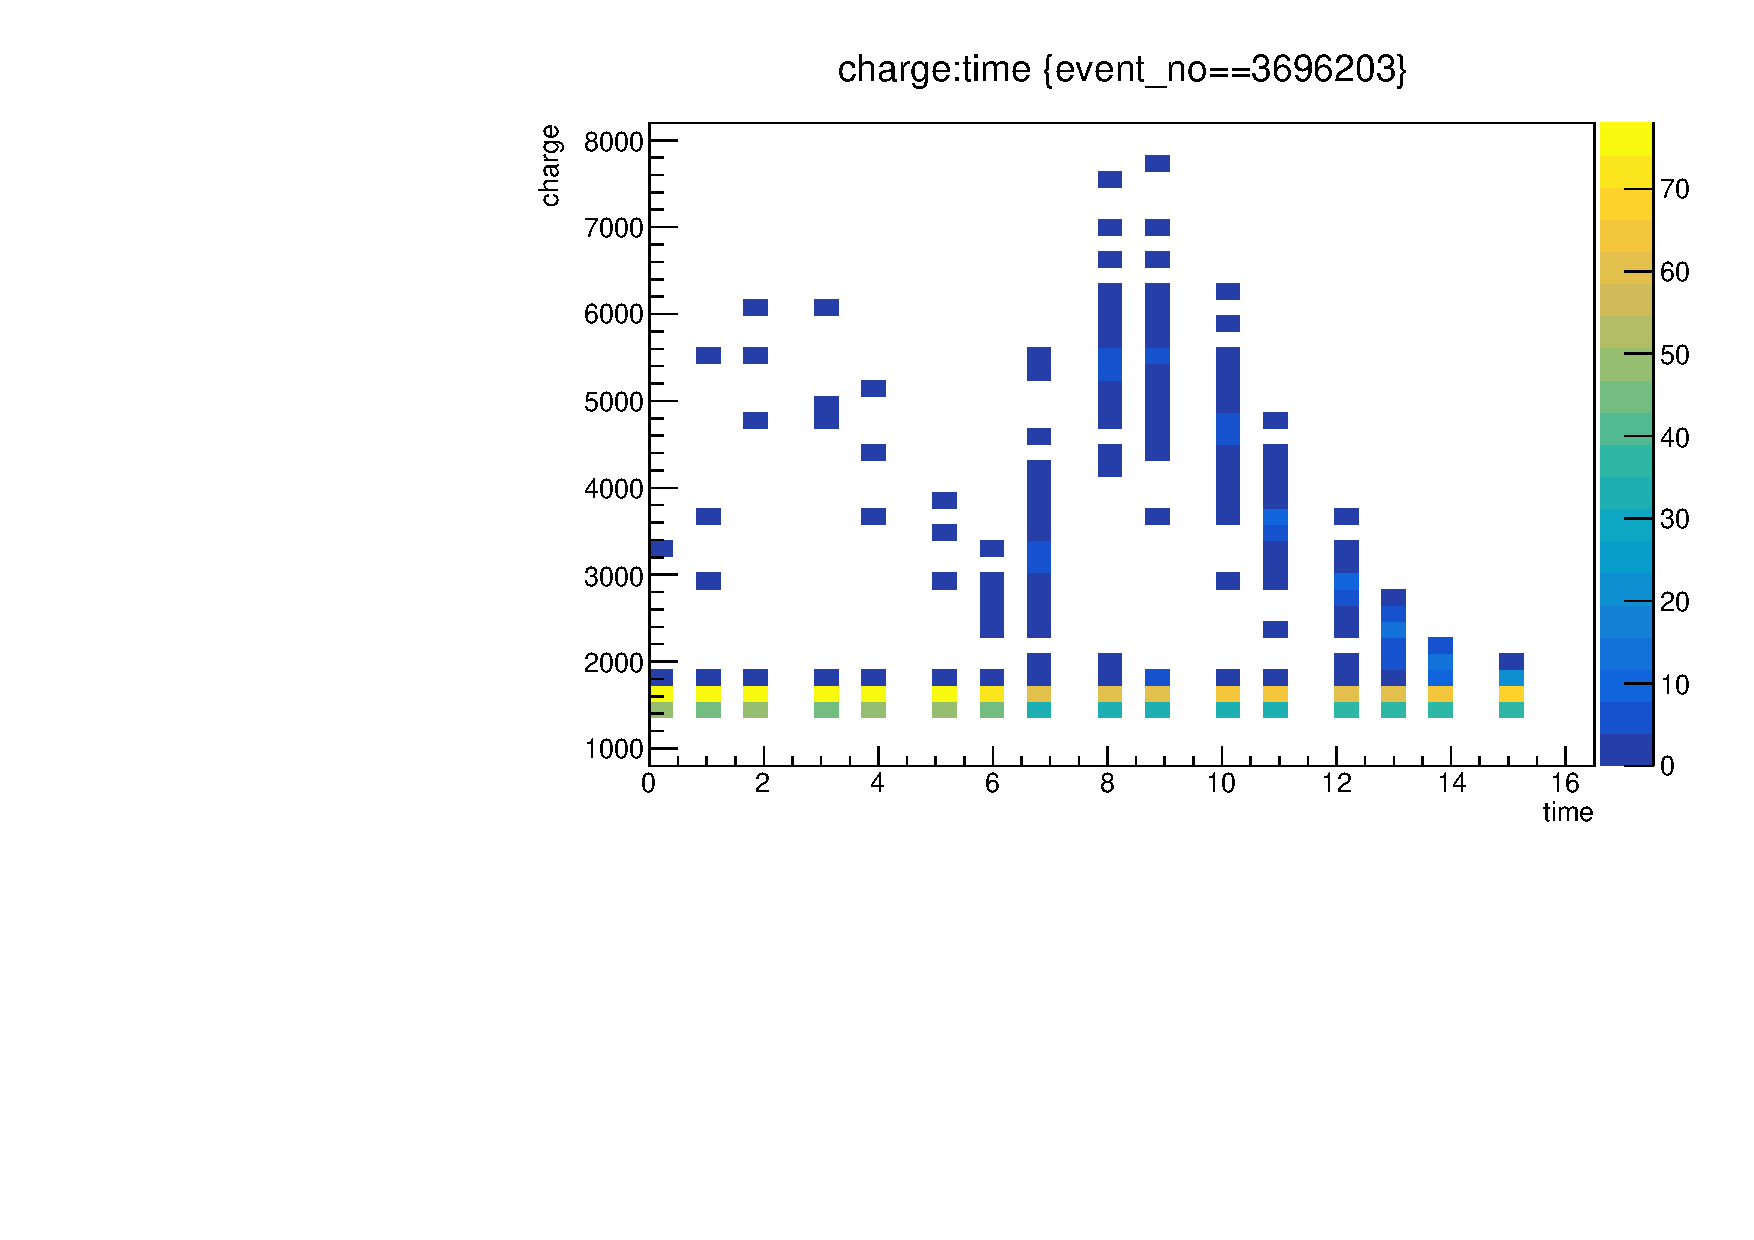
\includegraphics[width=1.\textwidth]{Figures/mbd_waveforms_pileup/MBD_2D_evt3696203.pdf}
    \end{subfigure}
    \begin{subfigure}{.329\textwidth}
    \centering
        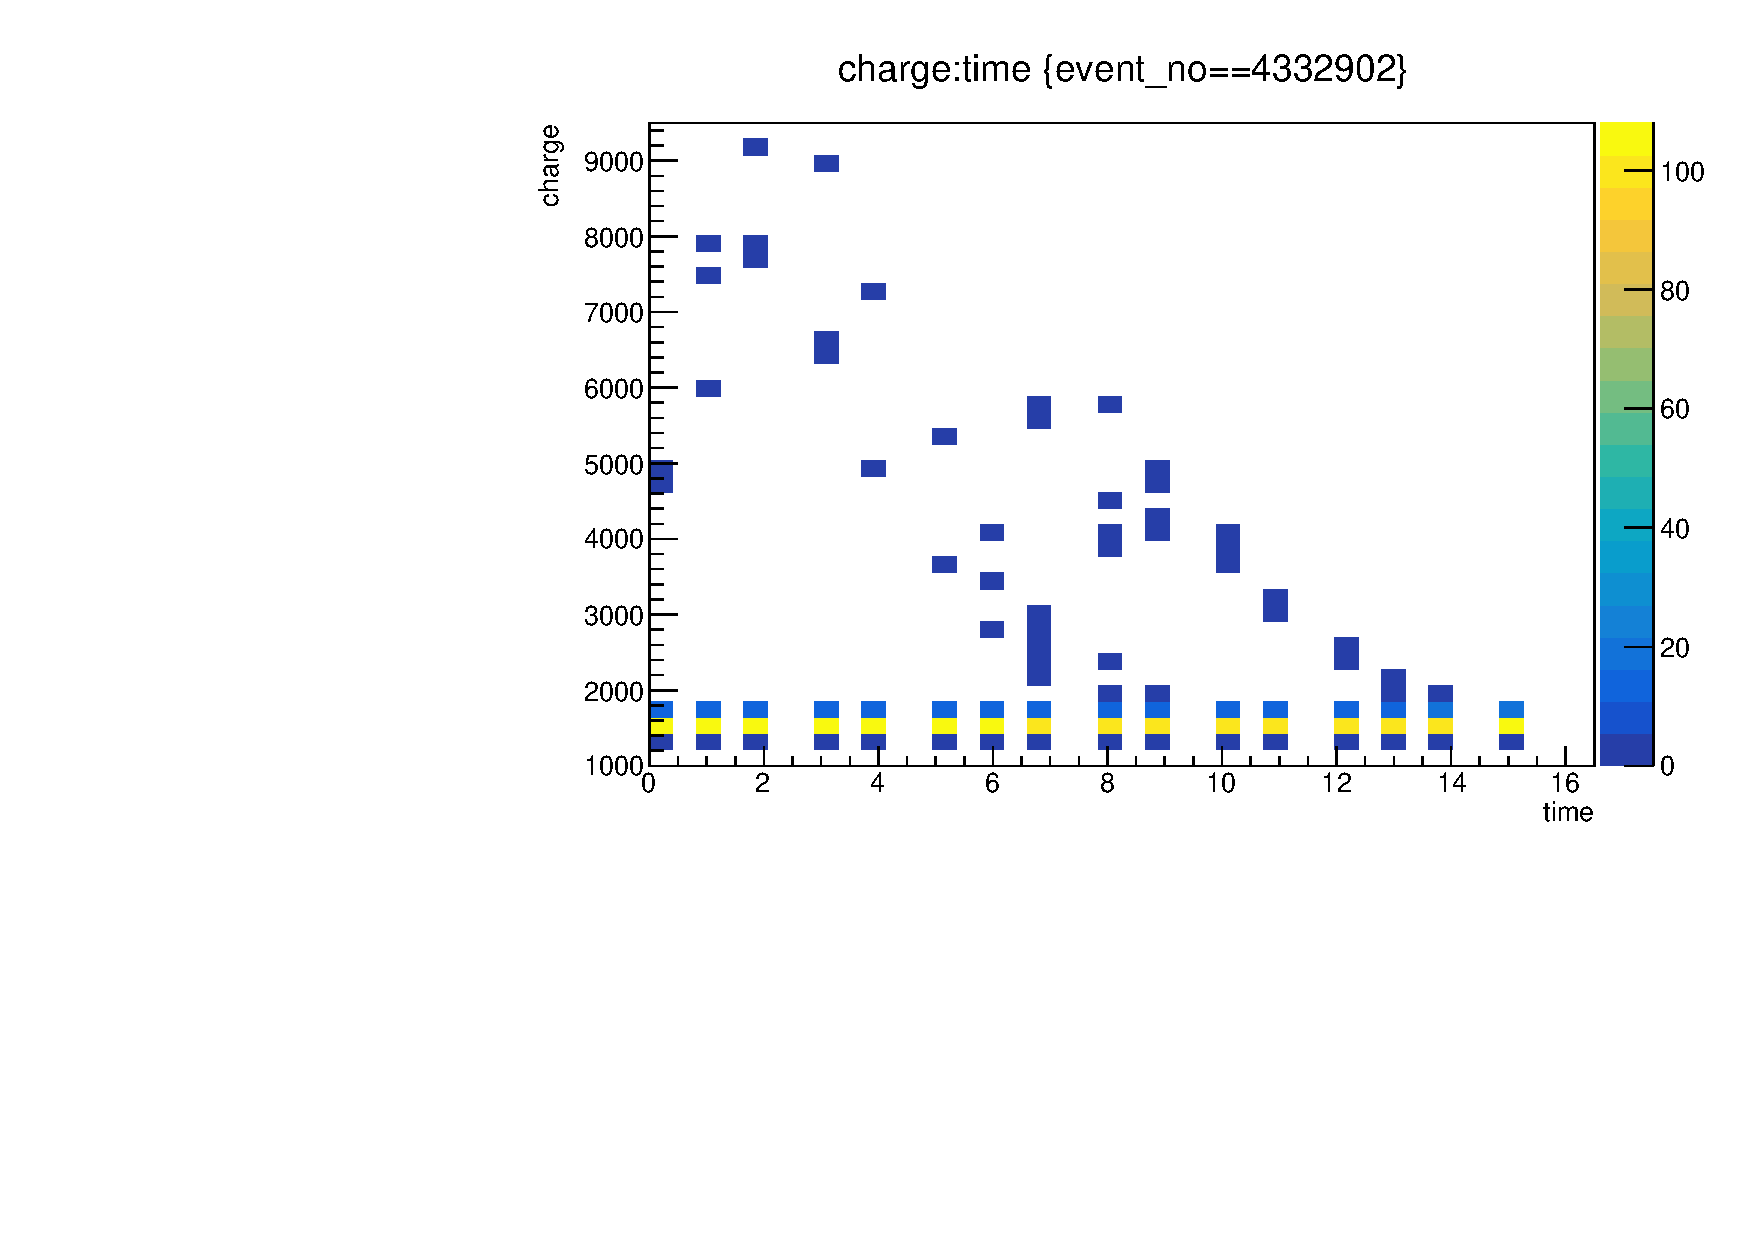
\includegraphics[width=1.\textwidth]{Figures/mbd_waveforms_pileup/MBD_2D_evt4332902.pdf}
    \end{subfigure}

    \begin{subfigure}{.329\textwidth}
    \centering
      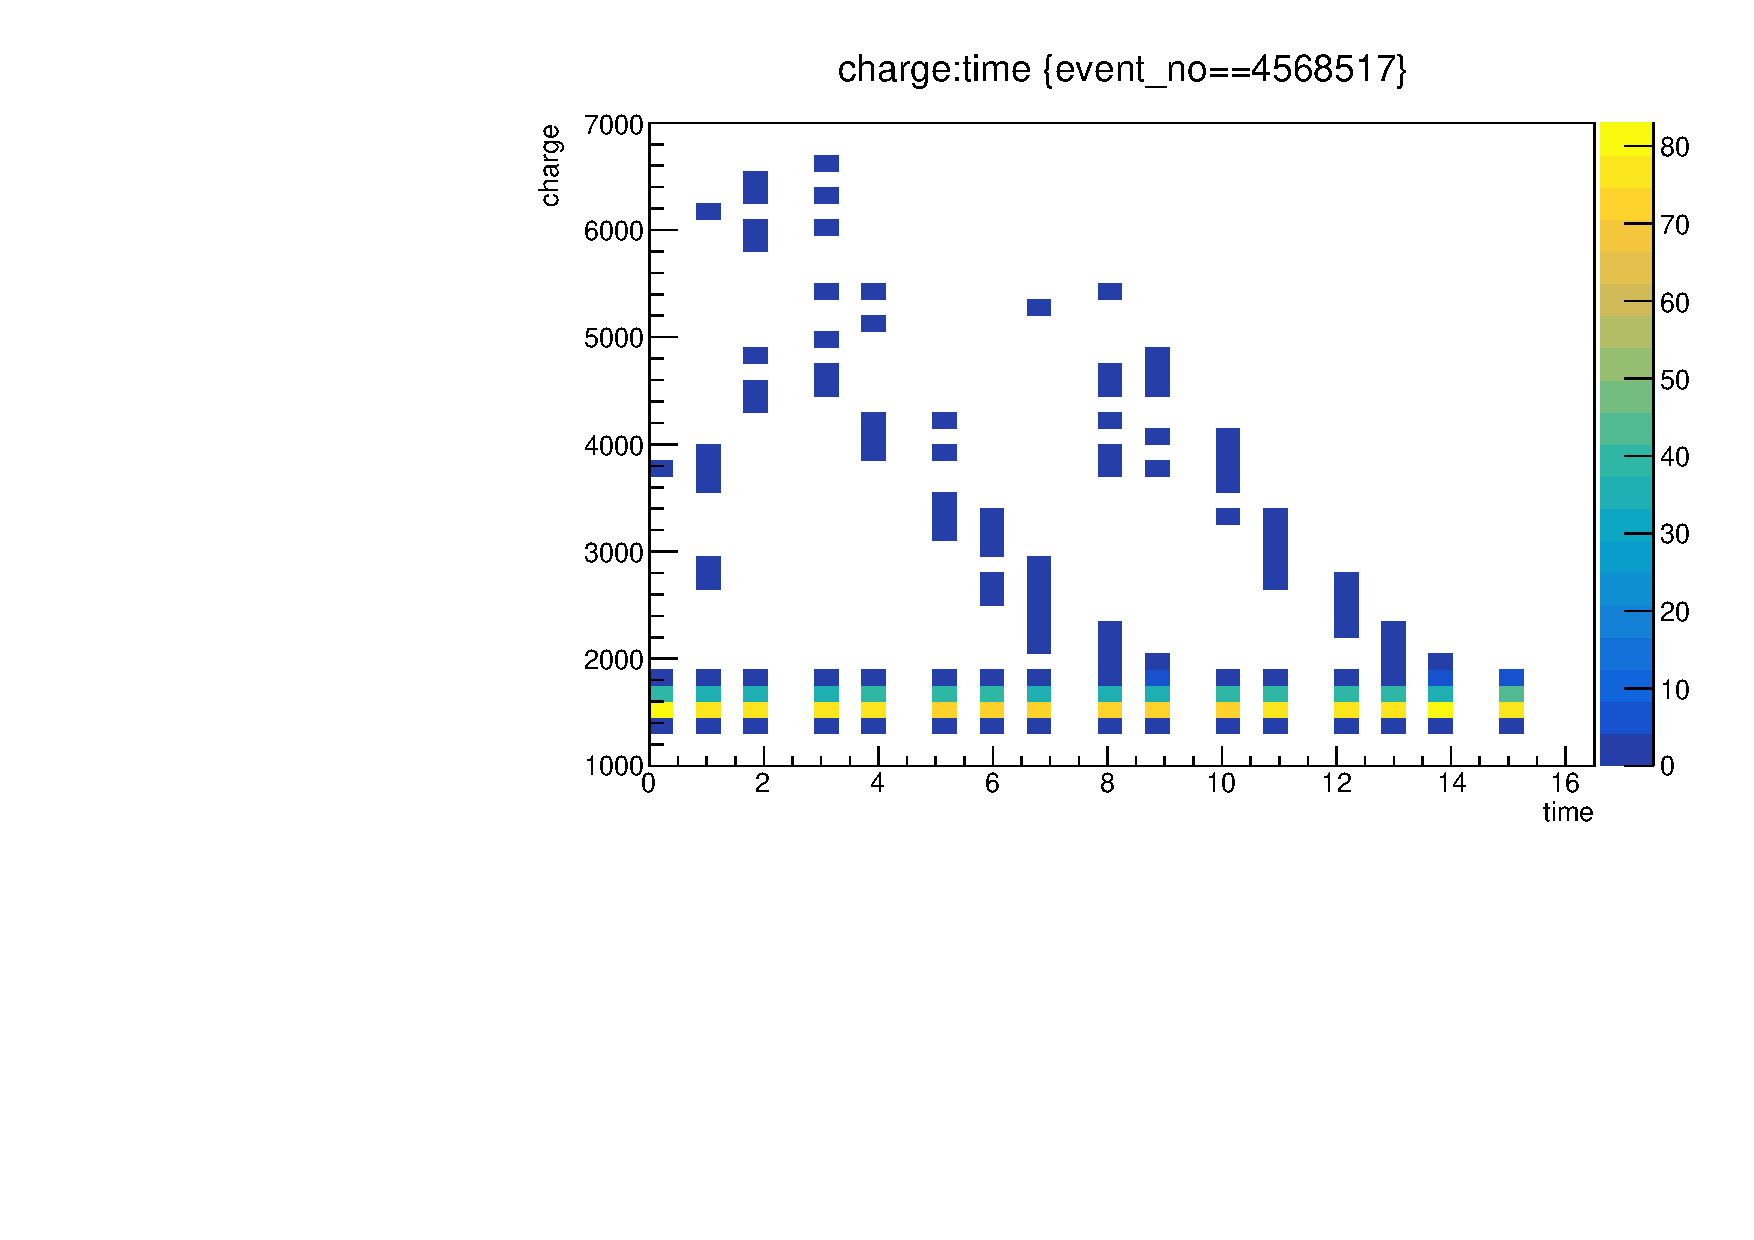
\includegraphics[width=1.\textwidth]{Figures/mbd_waveforms_pileup/MBD_2D_evt4568517.pdf}
    \end{subfigure}
    \begin{subfigure}{.329\textwidth}
    \centering
        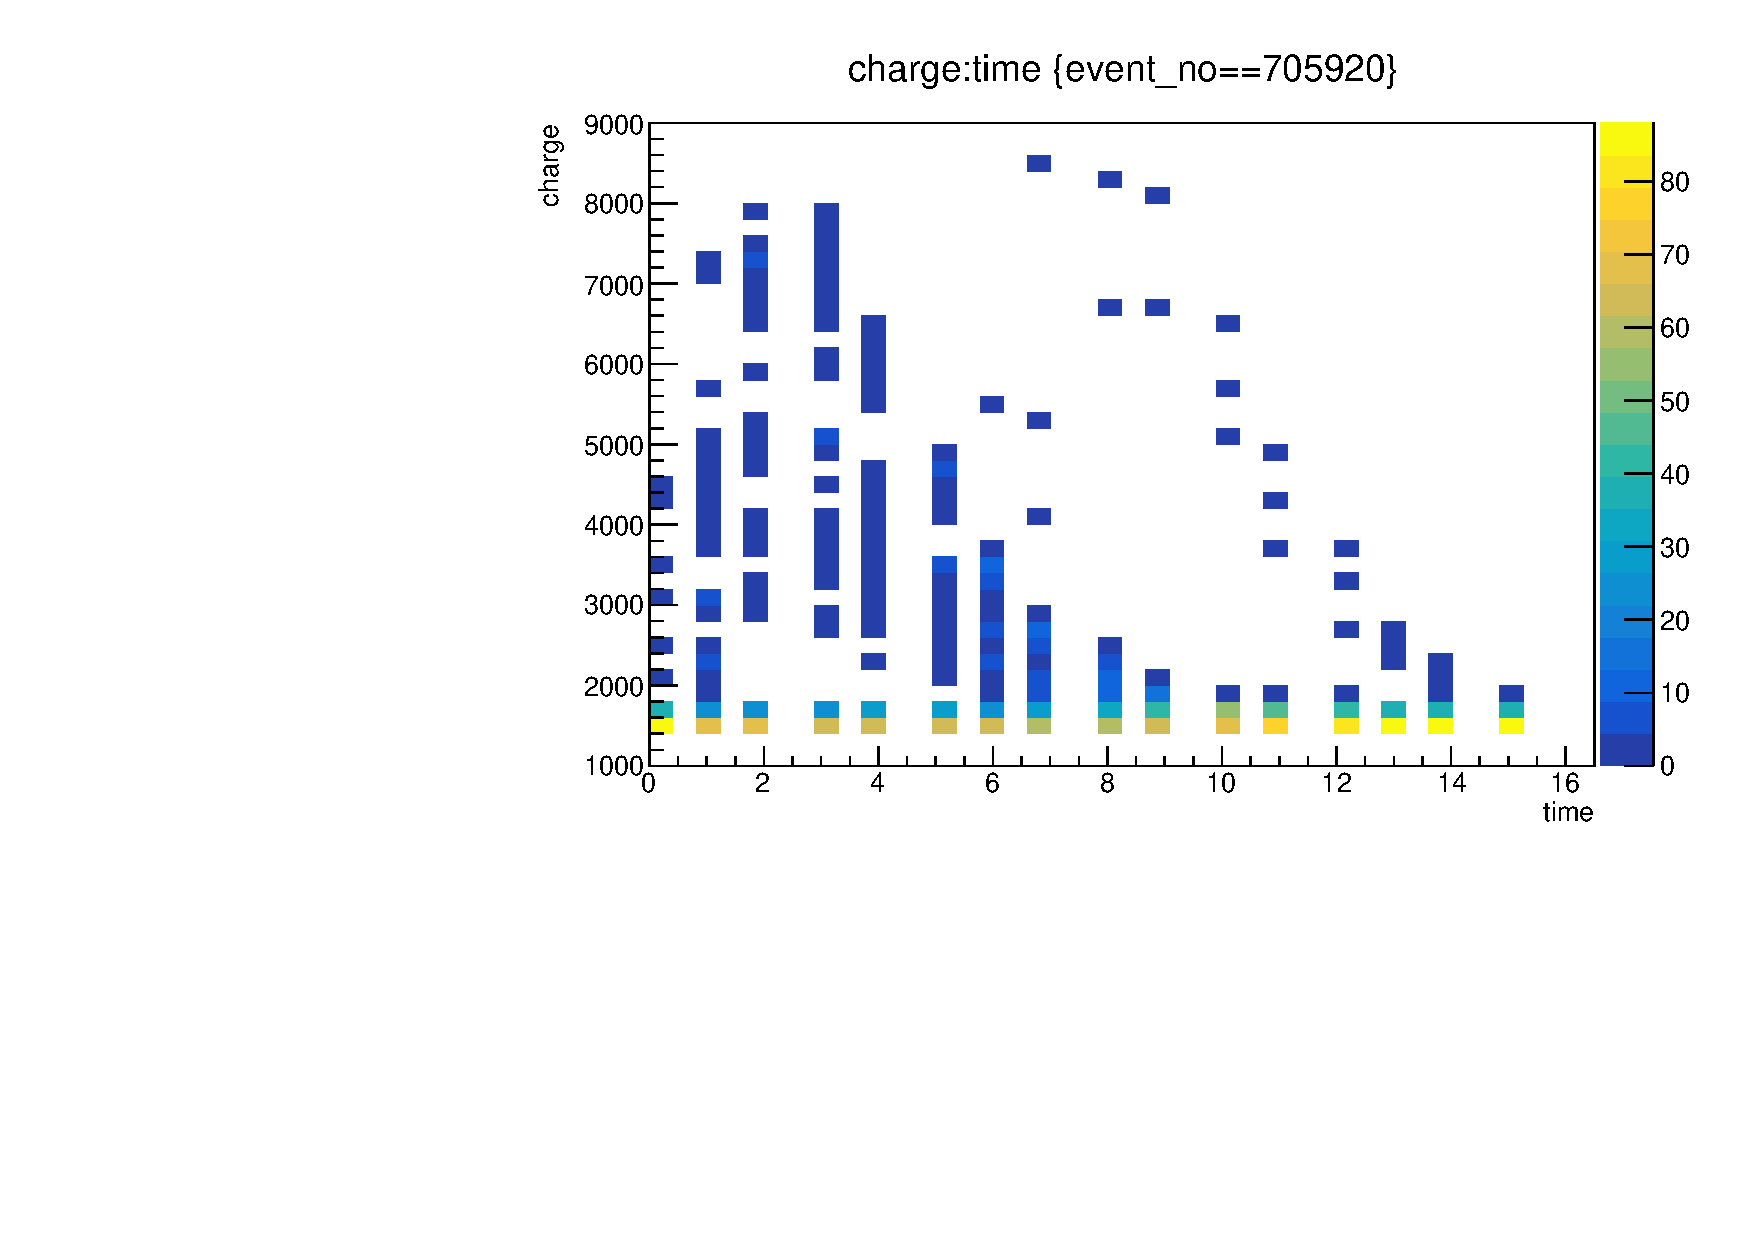
\includegraphics[width=1.\textwidth]{Figures/mbd_waveforms_pileup/MBD_2D_evt705920.pdf}
    \end{subfigure}
    \begin{subfigure}{.329\textwidth}
    \centering
        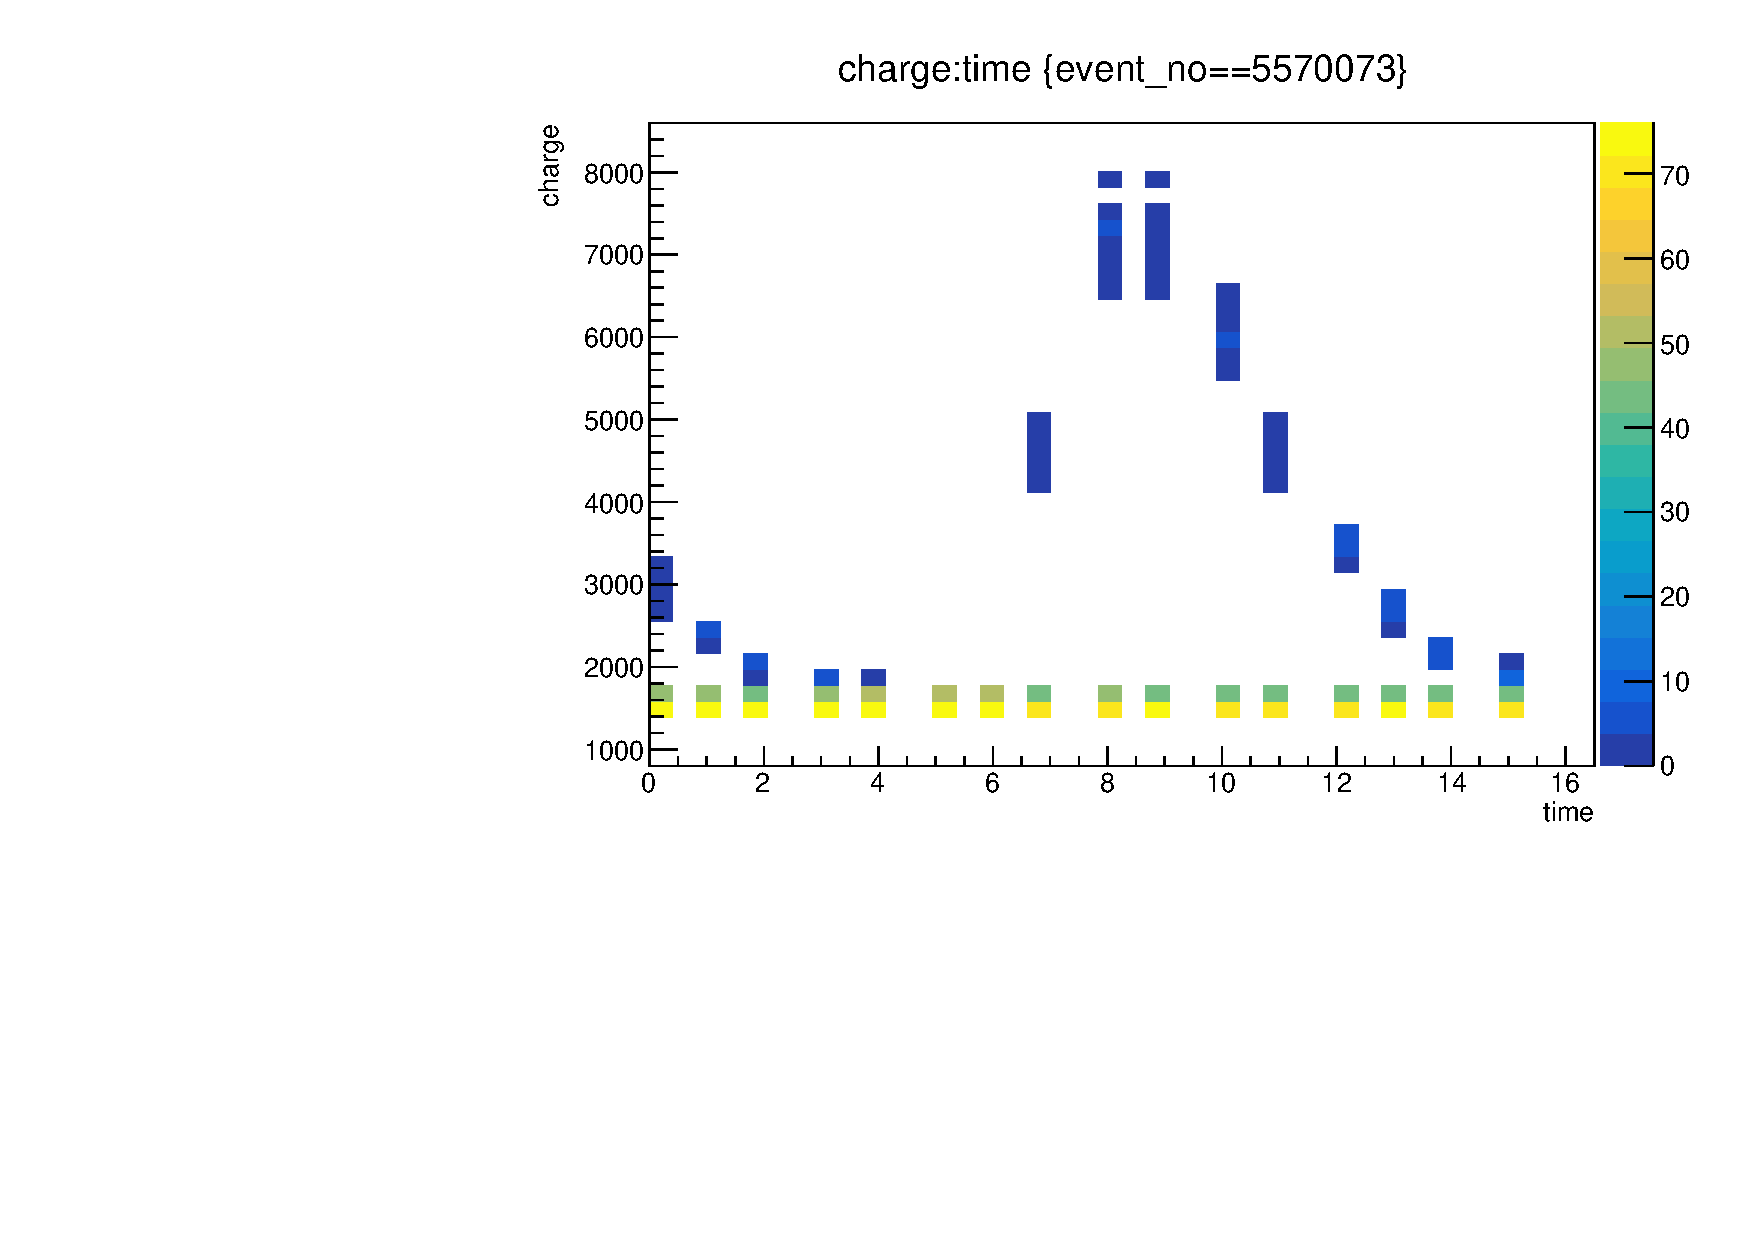
\includegraphics[width=1.\textwidth]{Figures/mbd_waveforms_pileup/MBD_2D_evt5570073.pdf}
    \end{subfigure}

    \begin{subfigure}{.329\textwidth}
    \centering
      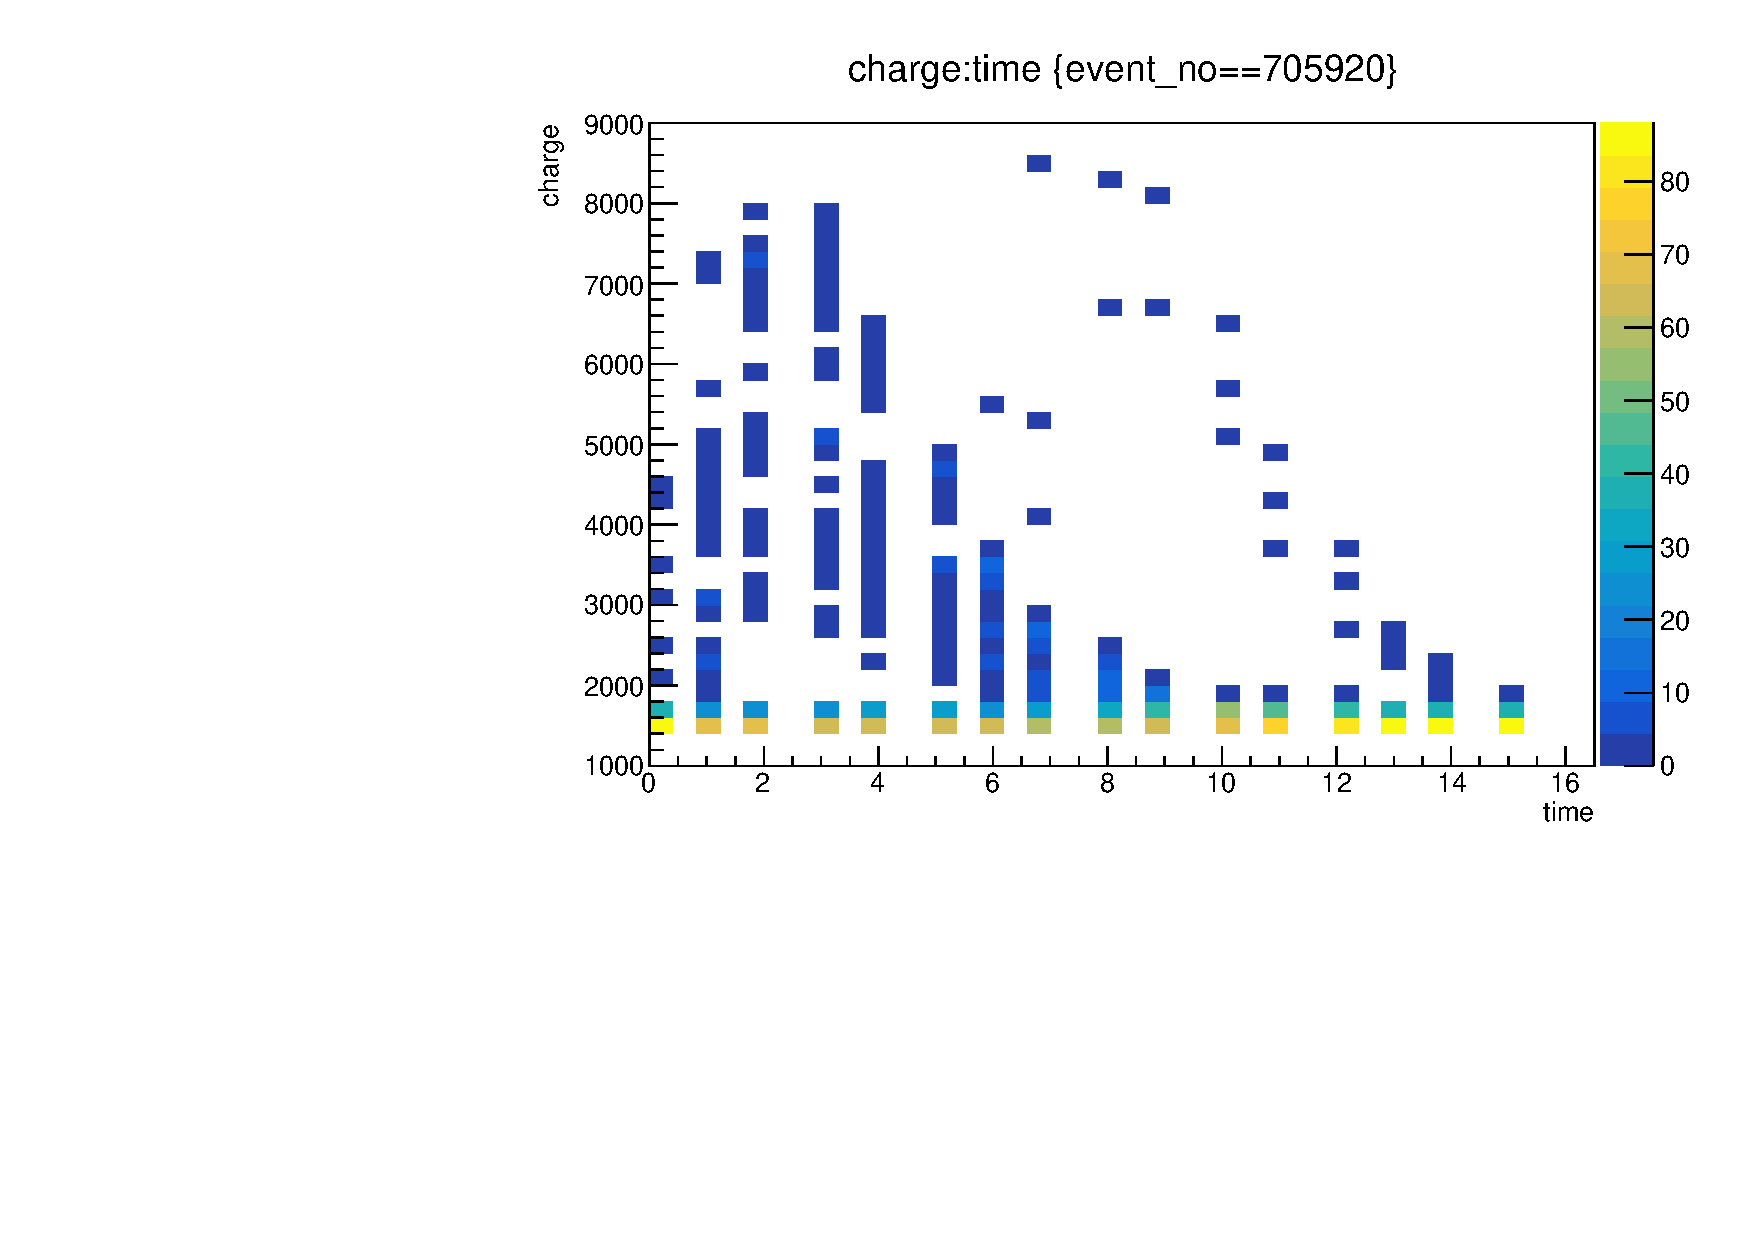
\includegraphics[width=1.\textwidth]{Figures/mbd_waveforms_pileup/MBD_2D_evt705920.pdf}
    \end{subfigure}
    \begin{subfigure}{.329\textwidth}
    \centering
        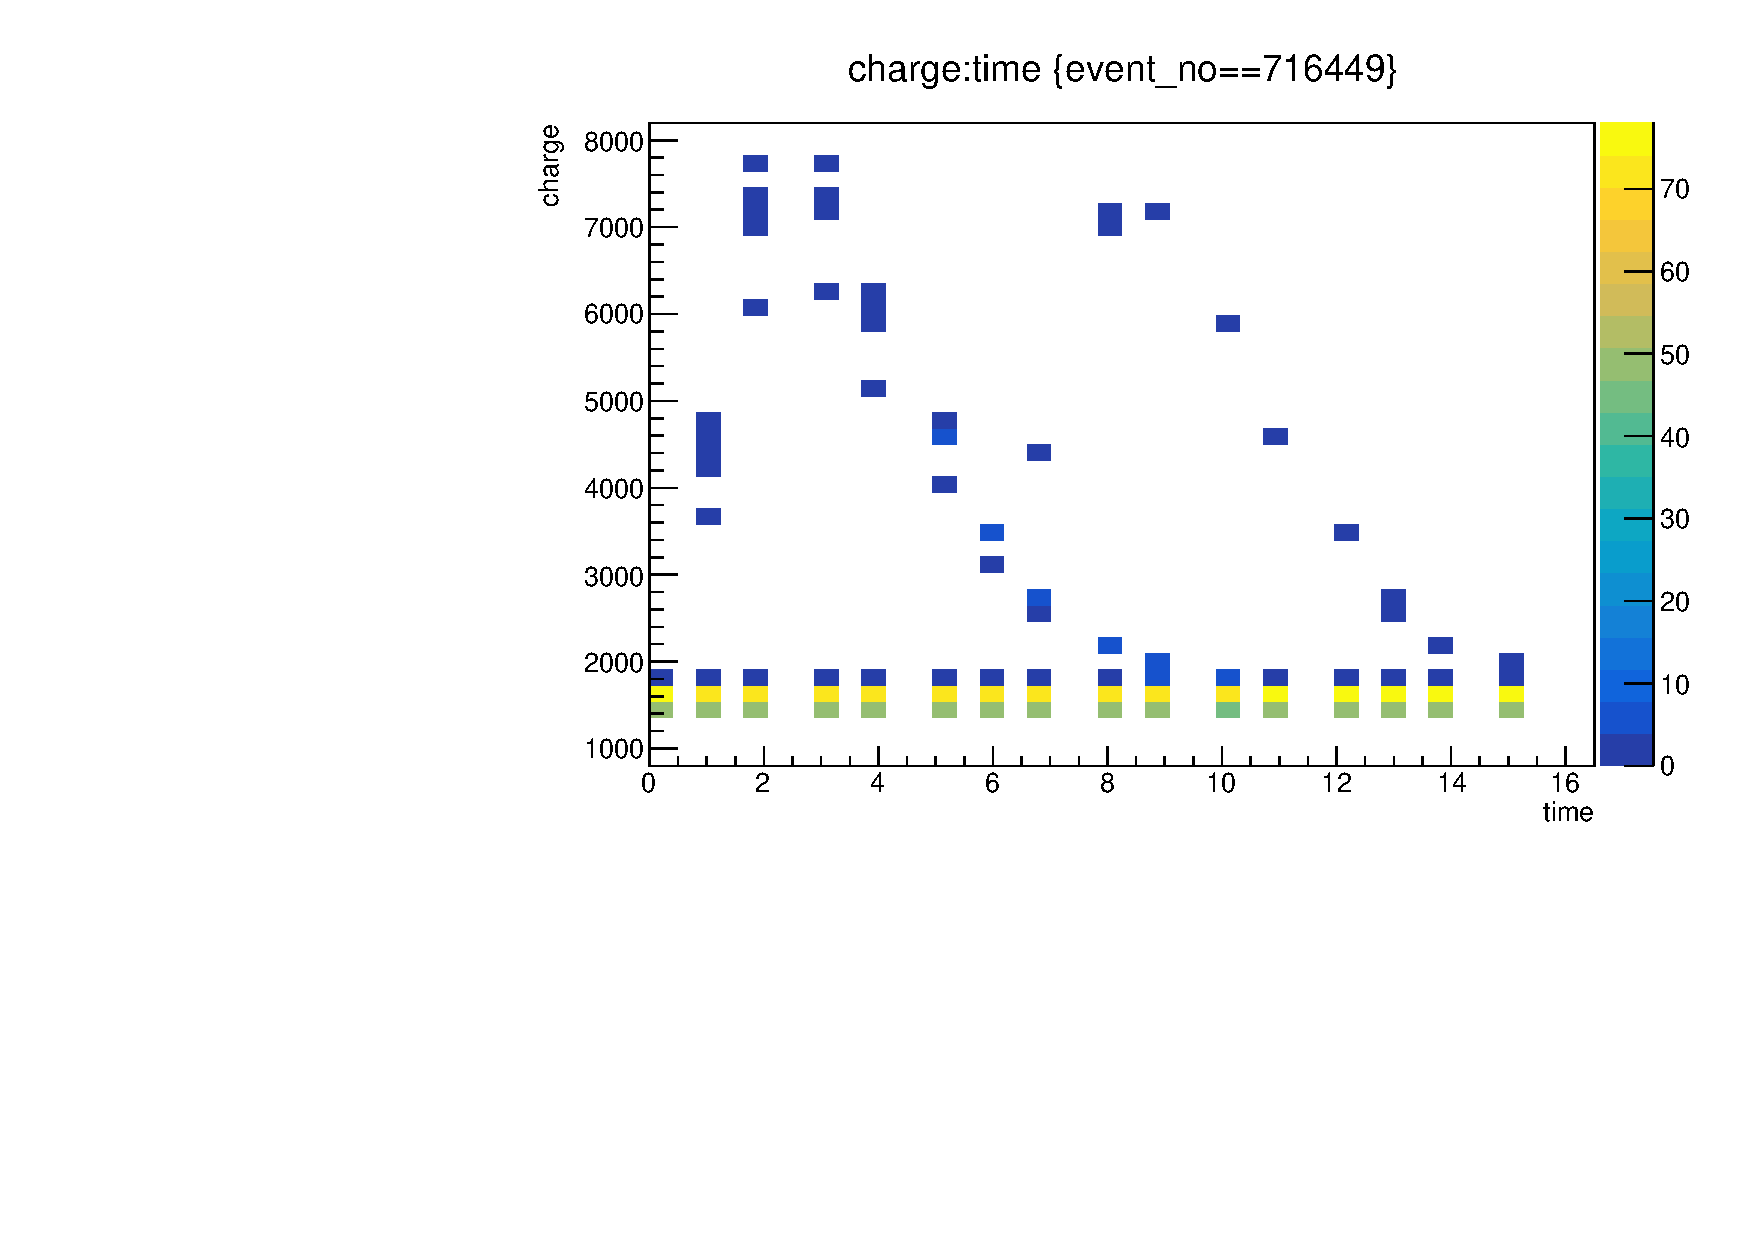
\includegraphics[width=1.\textwidth]{Figures/mbd_waveforms_pileup/MBD_2D_evt716449.pdf}
    \end{subfigure}
    \begin{subfigure}{.329\textwidth}
    \centering
        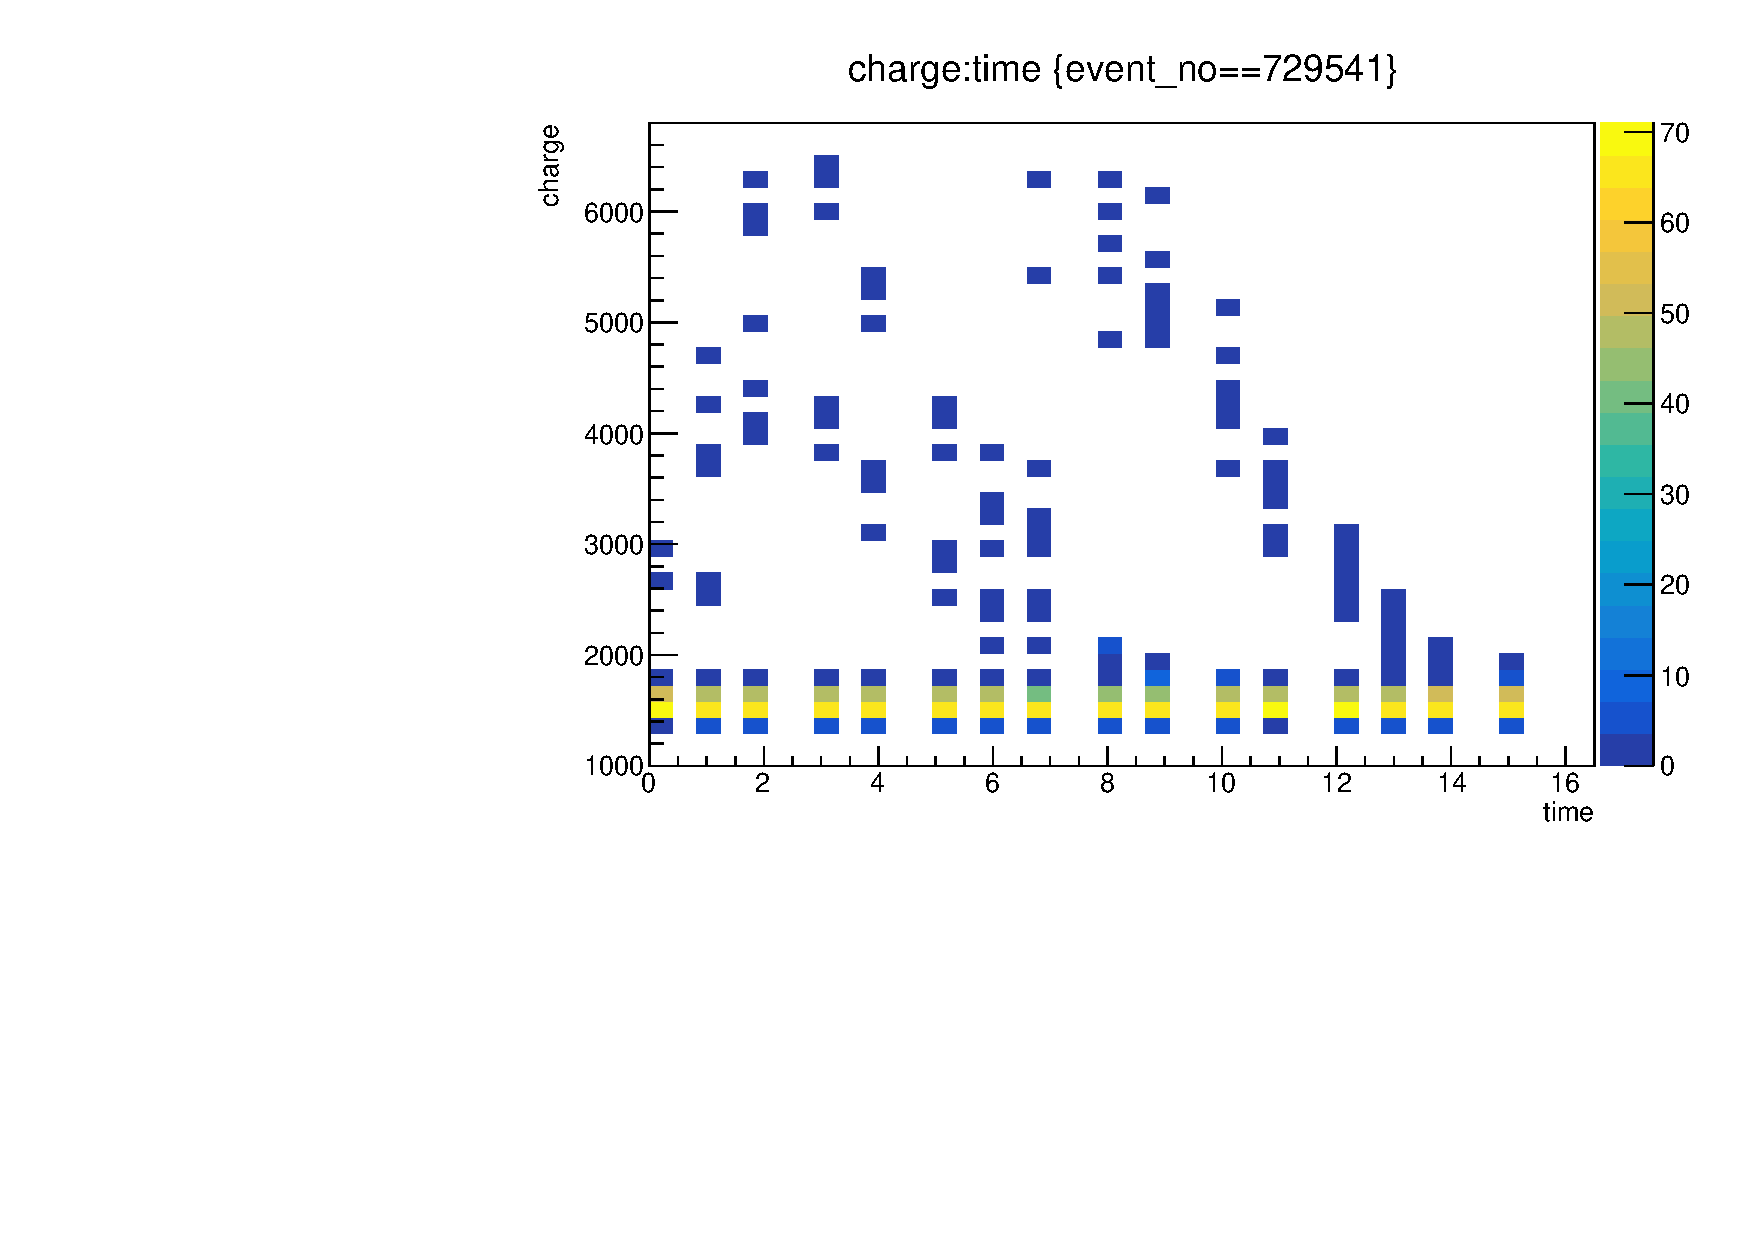
\includegraphics[width=1.\textwidth]{Figures/mbd_waveforms_pileup/MBD_2D_evt729541.pdf}
    \end{subfigure}
    
    \caption{MBD waveform plots for 12 of the 66 events in run 49219 which contained an OHCal tower with energy below --3 GeV.}
\label{fig:MBD_2D_waveforms}
\end{figure}

%%  DISCUSS CORRECTION:
%%  - plot spectra for sum(E) > or < 0
%%  - determine E-value at which sum(E) < 0 spectra becomes dominant (~5x the positive sum(E) spectra) 
%%  - place min tower E-value
%%  - effect on observables (Emma???)
